\documentclass[fleqn,usenatbib]{mnras}
% \documentclass[linenumbers, twocolumn],
%a4paper 10pt]{aastex63}
\usepackage{float}
\usepackage[switch]{lineno}
% Depending on your LaTeX fonts installation, you might get better results with one of these:
%\usepackage{mathptmx}
%\usepackage{txfonts}
\usepackage{cancel}
% Use vector fonts, so it zooms properly in on-screen viewing software
% Don't change these lines unless you know what you are doing
\usepackage[T1]{fontenc}
\usepackage{ae,aecompl}
\usepackage{tabularx}
    \newcolumntype{L}{>{\raggedright\arraybackslash}X}
\usepackage{placeins}
\usepackage{float}

\usepackage{graphicx,epstopdf}
\epstopdfsetup{suffix=}
\DeclareGraphicsExtensions{.ps}
\DeclareGraphicsRule{.ps}{pdf}{.pdf}{`ps2pdf -dEPSCrop -dNOSAFER #1 \noexpand\OutputFile}

\usepackage{amsmath}	% Advanced maths commands
\usepackage{amssymb}	% Extra maths symbols
\usepackage{mathtools}
\usepackage{longtable}
\usepackage{subfigure}
\usepackage{natbib}
\usepackage{adjustbox}
\usepackage{multirow}
\usepackage{tikz}
\usetikzlibrary{shapes.geometric, arrows}

\usepackage{hyperref}


\usepackage{newtxtext,newtxmath}
% \documentclass{article}
%\usepackage[square,numbers]{natbib}
% \bibliographystyle{abbrvnat}
% \bibliographystyle{unsrt}
% \bibliographystyle{habbrv}
\usepackage{graphicx}%Include figure files
\usepackage{mathtools}
\usepackage{ulem}
\usepackage{scrextend}
\usepackage{caption}
\usepackage{chngcntr}
\definecolor{mygreen}{RGB}{25, 196, 139}
% \usepackage[dvipsnames]{xcolor}
% \usepackage{multicol}

% \usepackage{caption}
%\usepackage{longtable}
%\usepackage{subcaption}
% easy way to highlight new stuff

\newcommand{\tatiana}[1]{{\color{orange} #1}}
\newcommand{\ggd}[1]{{\color{violet}\bf (GGD: #1)}}
\newcommand{\greg}[1]{{\color{violet} #1}}
\newcommand{\fed}[1]{{\color{orange} #1}}
\newcommand{\helen}[1]{{\color{magenta} #1}}
\newcommand{\masao}[1]{{\color{green} #1}}
\newcommand{\diff}{{\it diff}}

\newcommand{\nodia}{{\it noDIA}}
\newcommand{\diabased}{{\it DIA-based}}
\newcommand{\temp}{{\it tmpl}}
\newcommand{\search}{{\it srch}}
\newcommand{\question}[1]{{\color{red} #1}}
\newcommand{\new}[1]{{\color{purple} #1}}
\newcommand{\eg}{{\it e.g.}}
\newcommand{\ie}{{\it i.e.}}
\newcommand{\tsne}{t-SNE}
\newcommand{\idiff}{\ensuremath{I_\mathrm{diff}}}
\newcommand{\itempl}{\ensuremath{I_\mathrm{tmpl}}}
\newcommand{\isearch}{\ensuremath{I_\mathrm{srch}}}


% \usepackage{minted}
\usepackage[finalizecache=true, frozencache=false]{minted}
% \usepackage[frozencache=true,cachedir=minted-cache]{minted}


%\begin{document}

% \title{temporary: Deep Learning Real-Bogus}

\title[noDIA]{There's no difference: Convolutional Neural Networks for transient detection without template subtraction}



% The list of authors, and the short list which is used in the headers.
% If you need two or more lines of authors, add an extra line using \newauthor
\author[]
{Tatiana Acero-Cuellar$^{1, 2}$,
%[0000-0003-1953-8727]
{Federica B. Bianco}$^{2,3,4,5}$,
Gregory Dobler$^{2,3,4,6}$, 
\newauthor
Masao Sako$^{7}$,
%\newauthor
Helen Qu$^{7}$ and 
The LSST Dark Energy Science Collaboration%0000-0003-2242-0244]
\\
% List of institutions
$^{1}$Observatorio Astronómio Nacional, Universidad Nacional de Colombia, Bogotá, Colombia \\
$^{2}${University of Delaware
Department of Physics and Astronomy
217 Sharp Lab
Newark, DE 19716 USA}\\
$^{3}${University of Delaware
Joseph R. Biden, Jr. School of Public Policy and Administration, 
184 Academy St, Newark, DE 19716 USA}\\
$^4${University of Delaware
Data Science Institute}\\
$^5${Rubin Observatory}\\
$^6${Center for Urban Science and Progress, New York University, 
370 Jay St, Brooklyn, NY 11201, USA}\\
$^{7}$Department of Physics and Astronomy, University of Pennsylvania, Philadelphia, PA 19104, USA\\
}


% \correspondingauthor{Tatiana Acero-Cuellar}
% \email{taceroc@unal.edu.co}
% \author{Tatiana Acero-Cuellar}
% \affiliation{Observatorio Astronómio Nacional, Universidad Nacional de Colombia, Bogotá, Colombia}
% \affiliation{Department of Physics and Astronomy, University of Delaware, Newark, DE 19716-2570, USA}

% \author{Federica B. Bianco}
% \affiliation{Department of Physics and Astronomy, University of Delaware, Newark, DE 19716-2570, USA}
% \affiliation{Biden School of Public Policy and Administration, University of Delaware, Newark, DE 19716-2570, USA}
% \affiliation{Data Science Institute, University of Delaware, Newark, DE 19716-2570, USA}

% \author{Gregory Dobler}
% \affiliation{Biden School of Public Policy and Administration, University of Delaware, Newark, DE 19716-2570, USA}
% \affiliation{Department of Physics and Astronomy, University of Delaware, Newark, DE 19716-2570, USA}
% \affiliation{Data Science Institute, University of Delaware, Newark, DE 19716-2570, USA}
% \author{Masao Sako}
% \affiliation{Department of Physics and Astronomy, University of Pennsylvania, Philadelphia, PA 19104, USA}
% \author{Helen Qu}
% \affiliation{Department of Physics and Astronomy, University of Pennsylvania, Philadelphia, PA 19104, USA}
% \author{(LSST Dark Energy Science Collaboration)}
\date{Accepted XXX. Received YYY; in original form ZZZ}

% Enter the current year, for the copyright statements etc.
\pubyear{2021}

% Don't change these lines
\begin{document}
\linenumbers
\label{firstpage}
\pagerange{\pageref{firstpage}--\pageref{lastpage}}
\maketitle


\begin{abstract}

We present a Convolutional Neural Network (CNN) model for the separation of astrophysical transients from image artifacts, a task known as ``real-bogus'' classification, that does not rely on Difference Image Analysis (DIA) which is a computationally expensive process involving image matching on small spatial scales in large volumes of data. We explore the use of CNNs to (1) automate the ``real-bogus'' classification, (2) reduce the computational costs of transient discovery. We compare the efficiency of two CNNs with similar architectures, one that uses ``image triplets'' (templates, search, and the corresponding difference image) and one that adopts a similar architecture but takes as input the template and search only. Without substantially changing the model architecture or retuning the hyperparameters to the new input, we observe only a small decrease in model efficiency (97\% to 92\% accuracy). We further investigate how the model that does not receive the difference image learns the required information from the template and search by exploring the saliency maps. Our work demonstrates that (1) CNNs are excellent models for ``real-bogus'' classification that rely exclusively on the imaging data and require no feature engineering task; (2) high-accuracy models can be built without the need to construct difference images. Since once trained, neural networks can generate predictions at minimal computational costs, we argue that future implementations of this methodology could dramatically reduce the computational costs in the detection of genuine transients in synoptic surveys like Rubin Observatory’s Legacy Survey of Space and Time by bypassing the DIA step entirely.

%We present a Convolutional Neural Network-based model for the separation of astrophysical transients from image artifacts, a task known as ``real-bogus'' classification, that does not rely on Difference Image Analysis (DIA). \new{The process of identify astrophysical transients is currently principally based on DIA, which is a computationally expensive process involving image matching on small spatial scales for large volumes of data}. Here we investigate if machine learning could be leverage to not only automate the real-bogus classification, but to reduce the computational costs of transient discovery. We built and compared the efficiency of two models with similar architectures, one that uses ``image triplets'' composed of templates, search images, as well as the corresponding difference image, as traditionally done, and one that adopts a similar architecture but takes as input the template and search images only. We observe a small decrease in model efficiency,  accuracy reducing from 97\% to 92\% (dropping from an AUC of 0.992 to 0.973), when we remove the difference image from input, even if the model architecture is originally designed to maximize the efficiency of the model that uses image triplets as input. We further investigate what information is used by each model by exploring the models’ saliency maps (maps of pixel importance) and conclude that the model based on image triplets relies primarily on the difference image when in the presence of a genuine transient, but, much like a human classifier, needs additional information extracted from the template and search images to classify artifacts. Our work demonstrates that (1) deep neural networks are excellent models for real-bogus classification that rely exclusively on the imaging data and require no feature engineering task; (2) high-accuracy models can be built without the need to construct difference images, the most computationally expensive step in the detection of astrophysical transients. Since, once trained, neural networks can generate predictions at minimal computational costs, we argue that future implementations of this methodology could dramatically reduce the computational and human processing costs in the detection of genuine transients in synoptic surveys like Rubin Observatory’s Legacy Survey of Space and Time.
%We trained a Convolutional Neural Network (CNN) with a input data of size $51\times102$ without difference images, and compared its performance to a model trained using the difference, search and template images.
% We provide some interpretability to the results obtained by the CNNs models visualizing the saliency maps and quantifying the localization in the whole map of the most relevant pixels for the final classification.
% Our work suggests that high-accuracy models can be built without the need to construct a difference images, the most computationally expensive step in the detection of transients. Future implementations of this methodology can dramatically reduce the computational and human processing costs in the detection of genuine transients in synoptic surveys like Rubin Observatory's Legacy Survey of Space and Time.
\end{abstract}

\section{Introduction} \label{sec:intro}
% \question{questions are in red}

% \new{new text is purple}

% \ggd{Greg's comments look like this}

% \greg{New text written or modified by Greg in this color violet}


Modern observational astronomy has shown us that the Universe is not static and immutable: to the contrary, it is a lively and dynamic system. We now know and understand a variety of different phenomena that can give rise to variations in the brightness and color of astrophysical objects, including explosive stellar death (supernovae, kilonovae, Gamma Ray Bursts, etc), less dramatic and powerful stellar variability (flares, pulsations), and variability arising from geometric effects (such as planetary transients and microlensing). The time scales for these phenomena range from seconds to years. When the variations are terminal –like supernovae– or stochastic –like stellar flares– they are referred to as ``transients''. 
Detecting optical astrophysical transients characteristically requires sequences of images across a significant temporal baseline. Surveys like the Dark Energy Survey \citep[DES]{DES} or the future Rubin Observatory Legacy Survey of Space and Time \citep[LSST]{lsst} search for spatially localized changes in brightness in patches of sky previously observed. 

Due to the rarity of astrophysical transients, a long baseline in conjunction with the observation of a large area of the sky is typically required to detect a statistically significant sample of transients like supernovae and individual examples of rare events, such as kilonovae.  The process itself is arduous and requires considerable human intervention at multiple stages. The first step is typically the creation of high quality templates of each region of the sky that is to be searched; the templates are then subtracted from nightly images, a process known in astrophysics as Difference Image Analysis (DIA) that was initially pioneered by \cite{Tomaney_1996} and then formalized by \cite{Alard_1998} and there is a rich history of subsequent improvements in the efficiency and accuracy of DIA models. Templates  (\temp) are typically constructed as stacks of high quality (favorable observing conditions) sky images. These high quality images must then be aligned with the ``today'' image, typically called the ``search image'' (\search), and degraded to match its Point Spread Function (PSF, which we note may vary across a single large field of view image) and scaled to match its brightness. The product generated by the subtraction of the template from the search image is the so-called ``difference image''   (\diff; see for example a description of the DIA processing pipeline for DES in \citealt{Kessler_2015}).
Transients can then be detected as clusters of adjacent pixels deviating significantly from the sky noise.
% The current way of classifying optical images is to construct the image called template, which, in the case of  uses (READ \cite{Kessler_2015}), then the difference image is the residual obtained by subtracting the template and the science images. Many problems behind this steps to get the final classification and taking into account the large amount of data collected every day, the process of labeled objects by human inspection turns out to be very inefficient.))))\\
% Furthermore, miss-classifications due to human or computational error could lead to miss new astrophysical objects. \\
However, even the best existing DIA algorithms produce difference images with large pixel value deviation from an ideal 0-average that would be expected if no changes occurred in a patch of sky. Transients, variable stars, and moving objects will result in detections, but also a typically large number of artifacts will be detected by these thresholding schemes.

 

Machine learning models offer an excellent opportunity to improve the efficiency of transient detection at this stage, automating the classification between ``real'' astrophysical transients and ``bogus'' artifacts: these models are often referred to as ``Real-Bogus'' (hereafter, RB). Generally, the applications of machine learning to this problem are based on the extraction of features from the (difference) images that are then fed to models like Random Forests, k-Nearest Neighbors, or Support Vector Machines \citep{Goldstein_2015, S_nchez_2019, Mong_2020}. These models have achieved high accuracy and enabled the discovery of transients at scale in larger synoptic surveys, for example in the Palomar Transient Factory \citep[PTF][]{bloom2012automating} and Zwicky Transient Facility \citep[ZTF][]{2019PASP..131c8002M}. 

The process of engineering features for machine learning models allows the experts to embed domain knowledge in models. In the case of RB classification, the features engineered to be used by models such as the ones described above usually rely on visual inspection of a subset of the data. However, these features may overlook abstract associations between image properties that can be effective for classification, and in fact, may be biased towards human perception and theoretical expectations. An alternative approach involves the use of models that can learn features directly from the data, such as Convolutional Neural Networks \citep[CNNs]{lecun1989generalization}.  Here, it is possible to train a model using the images themselves, skipping the step of feature-design entirely.

RB CNN-based models appeared in the literature as early as 2016 \citep{Cabrera_2016}, and they are typically based on the analysis of the difference images arising from the DIA. While neural networks may be computationally demanding in the training phase, the "feed-forward" classification that arises from a pre-trained model is typically rapid and computationally light,\footnote{although the model may require a large amount of memory to cache.} leaving DIA as the computational bottle-neck in the process of astrophysical transients' detection. Yet in principle, the entirety of the information content embedded in the \diff-\temp-\search\ image triplet is also contained in the \temp-\search\ image pair.  In this paper, we explore the use of CNNs as RB models %(models that separate ``real'' astrophysical transients from ``bogus'' artifacts), 
concentrating on the potential for building high-accuracy models that \textit{do not} require the construction of difference images.  

 This paper represents a first, critical step in the process of conceptualizing and realizing a DIA-free model for astrophysical transients. Here we demonstrate that Neural Networks can discriminate between astrophysical transients and artifacts without a difference image, while still relying on DIA for detection. This is the necessary premise for the complete elimination of DIA and, with this conclusion in hand, in future work we intend to develop models that will not rely on DIA for detection, and, finally, that will detect and characterize transients (measure magnitude) from the \temp-\search\ image pair only.

% \subsection{Template}

% \subsection{Difference image analysis}

% \subsection{Convolutional Neural Network}

% SHOR DESCRIPTION ??

% In this paper we compare two CNN models trained on the same DES Y1 data \citep{Goldstein_2015}, one using as input data the template, search, and difference images, and the other using only the template and the search images. The main purpose is to demonstrate that relative simple CNN models are able to classify as ``real'' and ``bogus'' with high accuracy transient observations, without the necessity of the difference image.In \autoref{stateofart} we discuss the history, approaches, and details of DIA in the literature, and in \autoref{sec:data} we present the DES data that we will use to build our ``real''/``bogus'' classification models.  In \autoref{sec:results} we show the results of building a model that does not use the difference image as input and compare its performance to one that does, and we conclude with a discussion of the broader implications for this work in light of upcoming surveys in \autoref{sec:conclusion}.\\ 

This paper is organized as follows: in \autoref{sec:intro}, the introduction, we briefly describe DIA process, examples of architectures, and input images for CNNs models on the literature and describe the importance of our work. In \autoref{stateofart} we discuss the history, approaches, and details of DIA in the literature. In \autoref{sec:data} we present the DES data that we will use to build our RB classification models and the pre-processing steps. In \autoref{sec:method} we presented some general aspects of CNN and illustrate the CNNs architectures used, in \autoref{subsec: saliency} we present, share and discuss in some insights into the model obtained enabled by saliency maps, as well as the method used to interpret the data decisions through saliency maps. In \autoref{sec:results} we show the results of building a model that does not use the difference image as input, named \nodia -based model and compare its performance to one that does, named \diabased\ model;  we outline future work in \autoref{sec:futurework} and we conclude with a discussion of the broader implications for this result in light of upcoming surveys.

This study is reproducible and all the code that supports the analysis presented here is available on a dedicated \texttt{GitHub} repository. \footnote{\url{https://github.com/taceroc/DIA_noDIA}.}
% in \autoref{sec:conclusion}.
\begin{figure*}

    \centering
    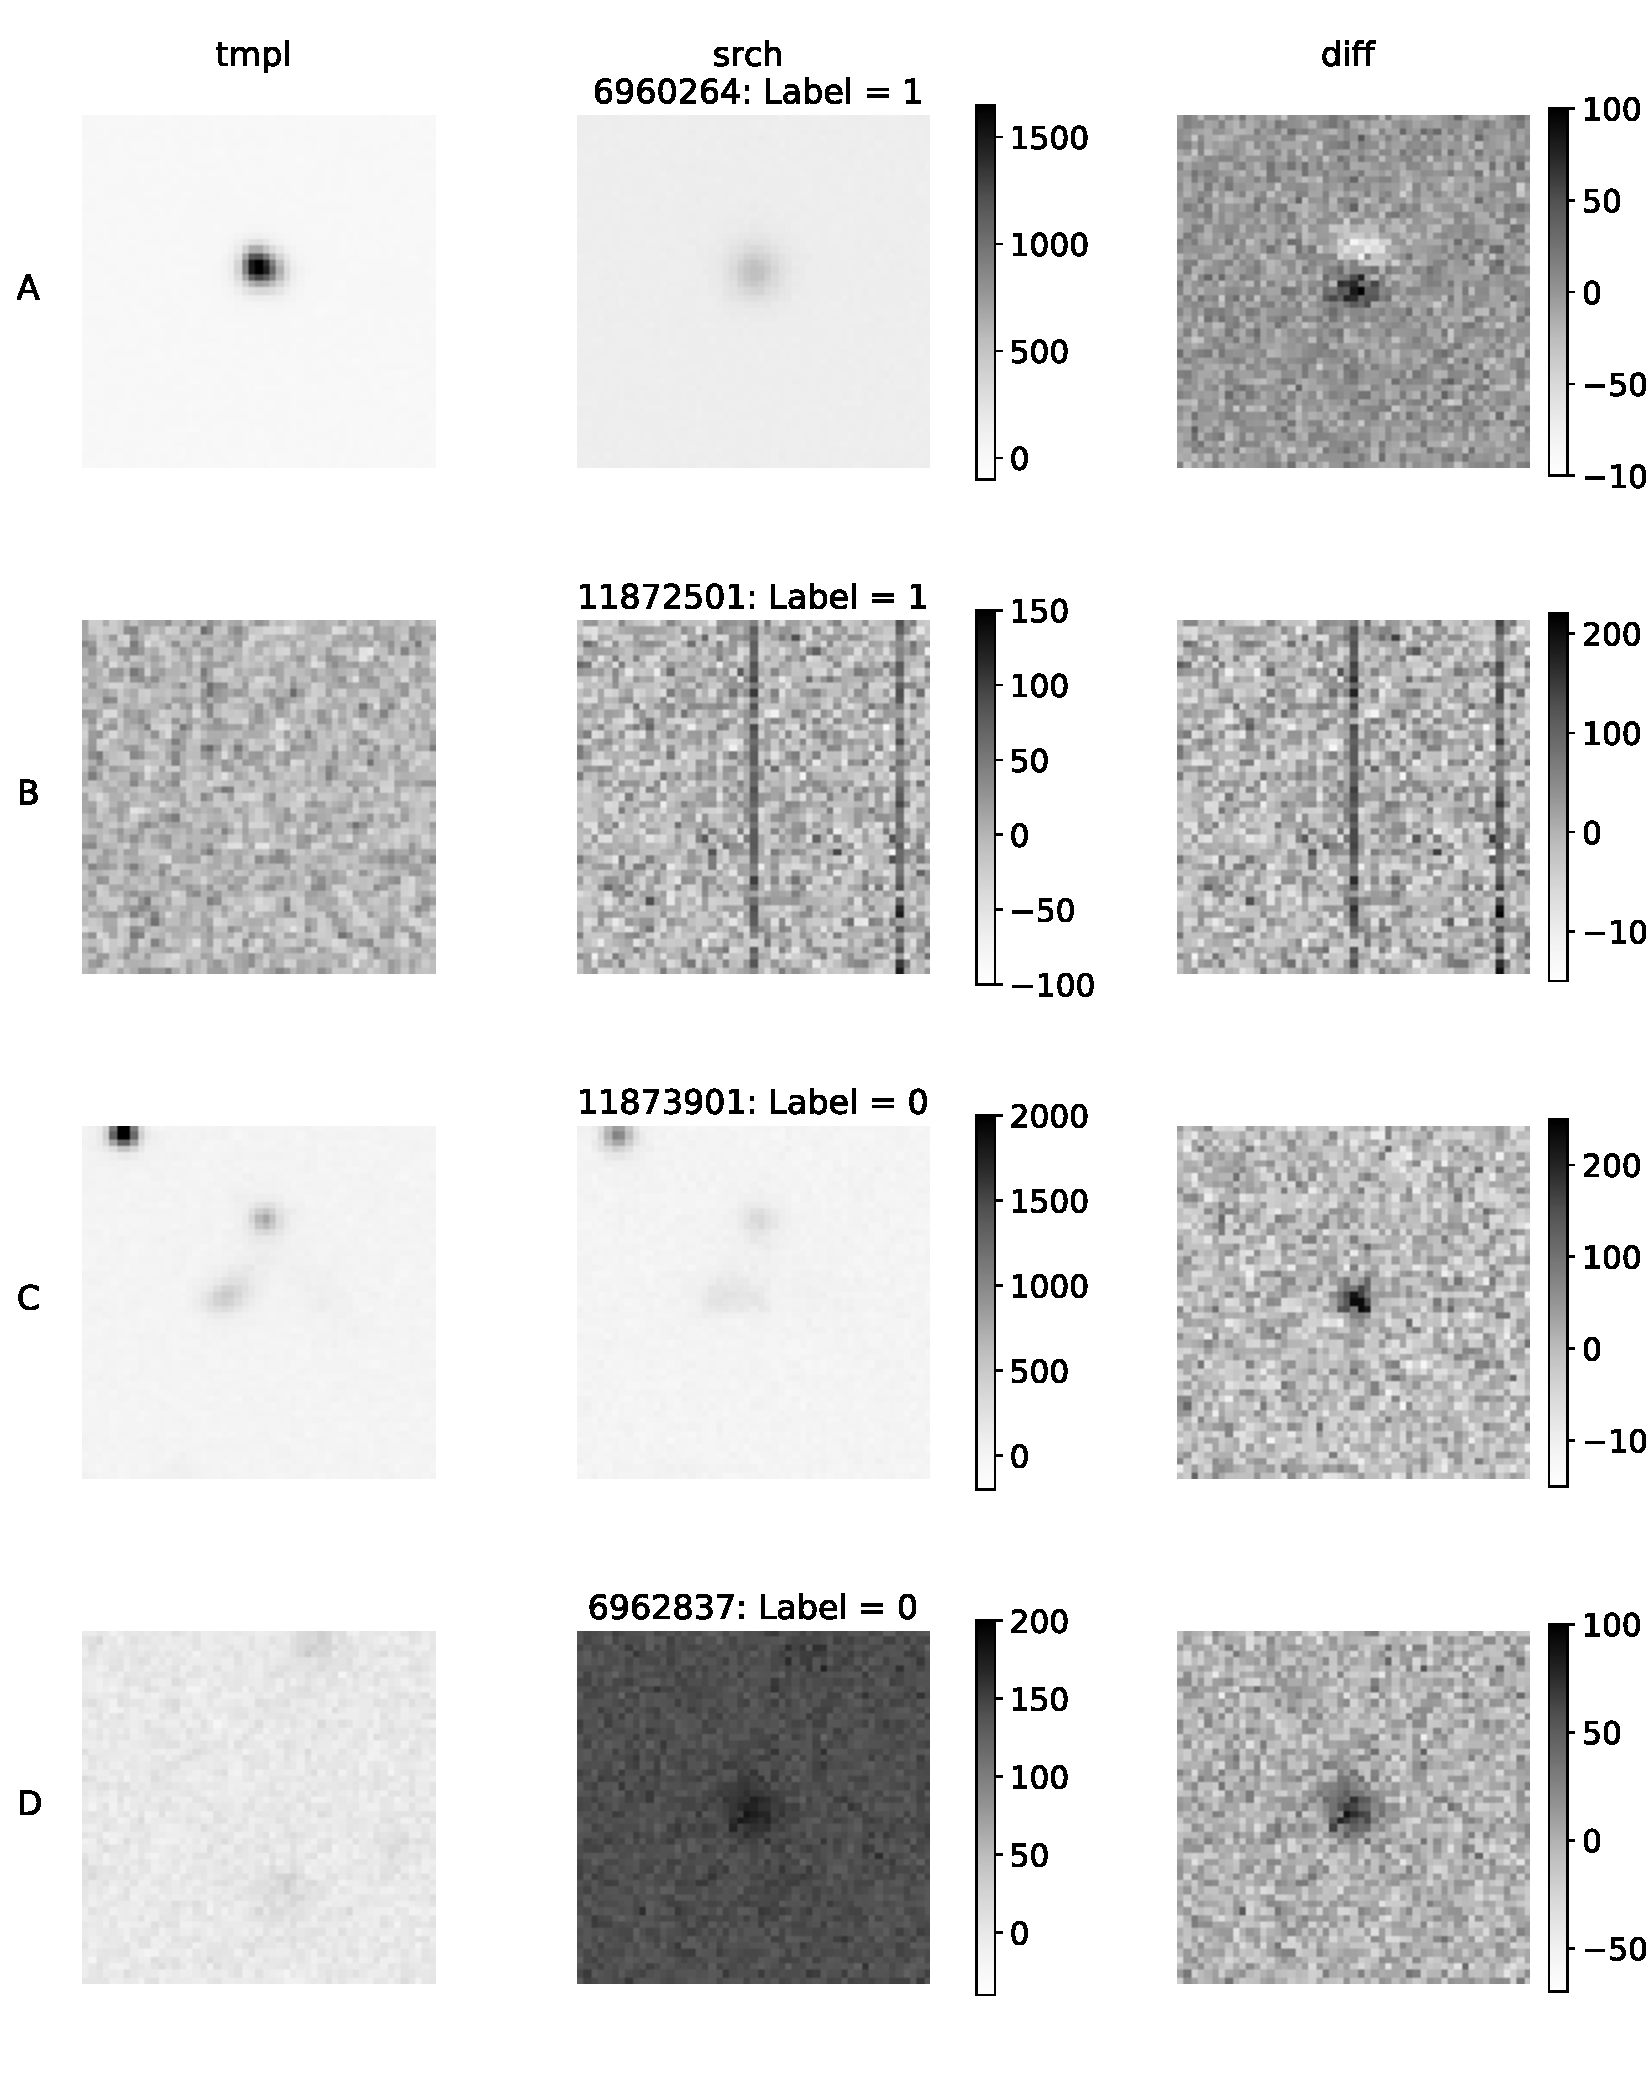
\includegraphics[width=0.52\linewidth]{figures/nonorm_new_test.pdf}
    \caption{Example of four DIA-sets from the first season of the Dark Energy Survey (DES): from left to right the images correspond to the template (\temp), search (\search), and difference (\diff) image; the \diff\ is generated as the subtraction of \temp\ and \search. Each pair of \temp\ and \search\ images is mapped to the same color range. We refer to these 3-images sets as ``image triplets'' or DIA-sets. A and B show artifacts, human-labeled as ``bogus'' (\texttt{label = 1}). C and D show transients labeled as ``real'' (\texttt{label = 0}).
     Above each triplet is the unique ID of the transient (see \citealt{Goldstein_2015})
    }
    \label{fig:examples_no_normalization}
\end{figure*}

%  in \autoref{sec:DI} we describe in more detail the Difference Imaging processes, in \autoref{sec:autoscan} we present relevant information about the precursor of our work \citep{Goldstein_2015},
\begin{figure*}
    \centering
    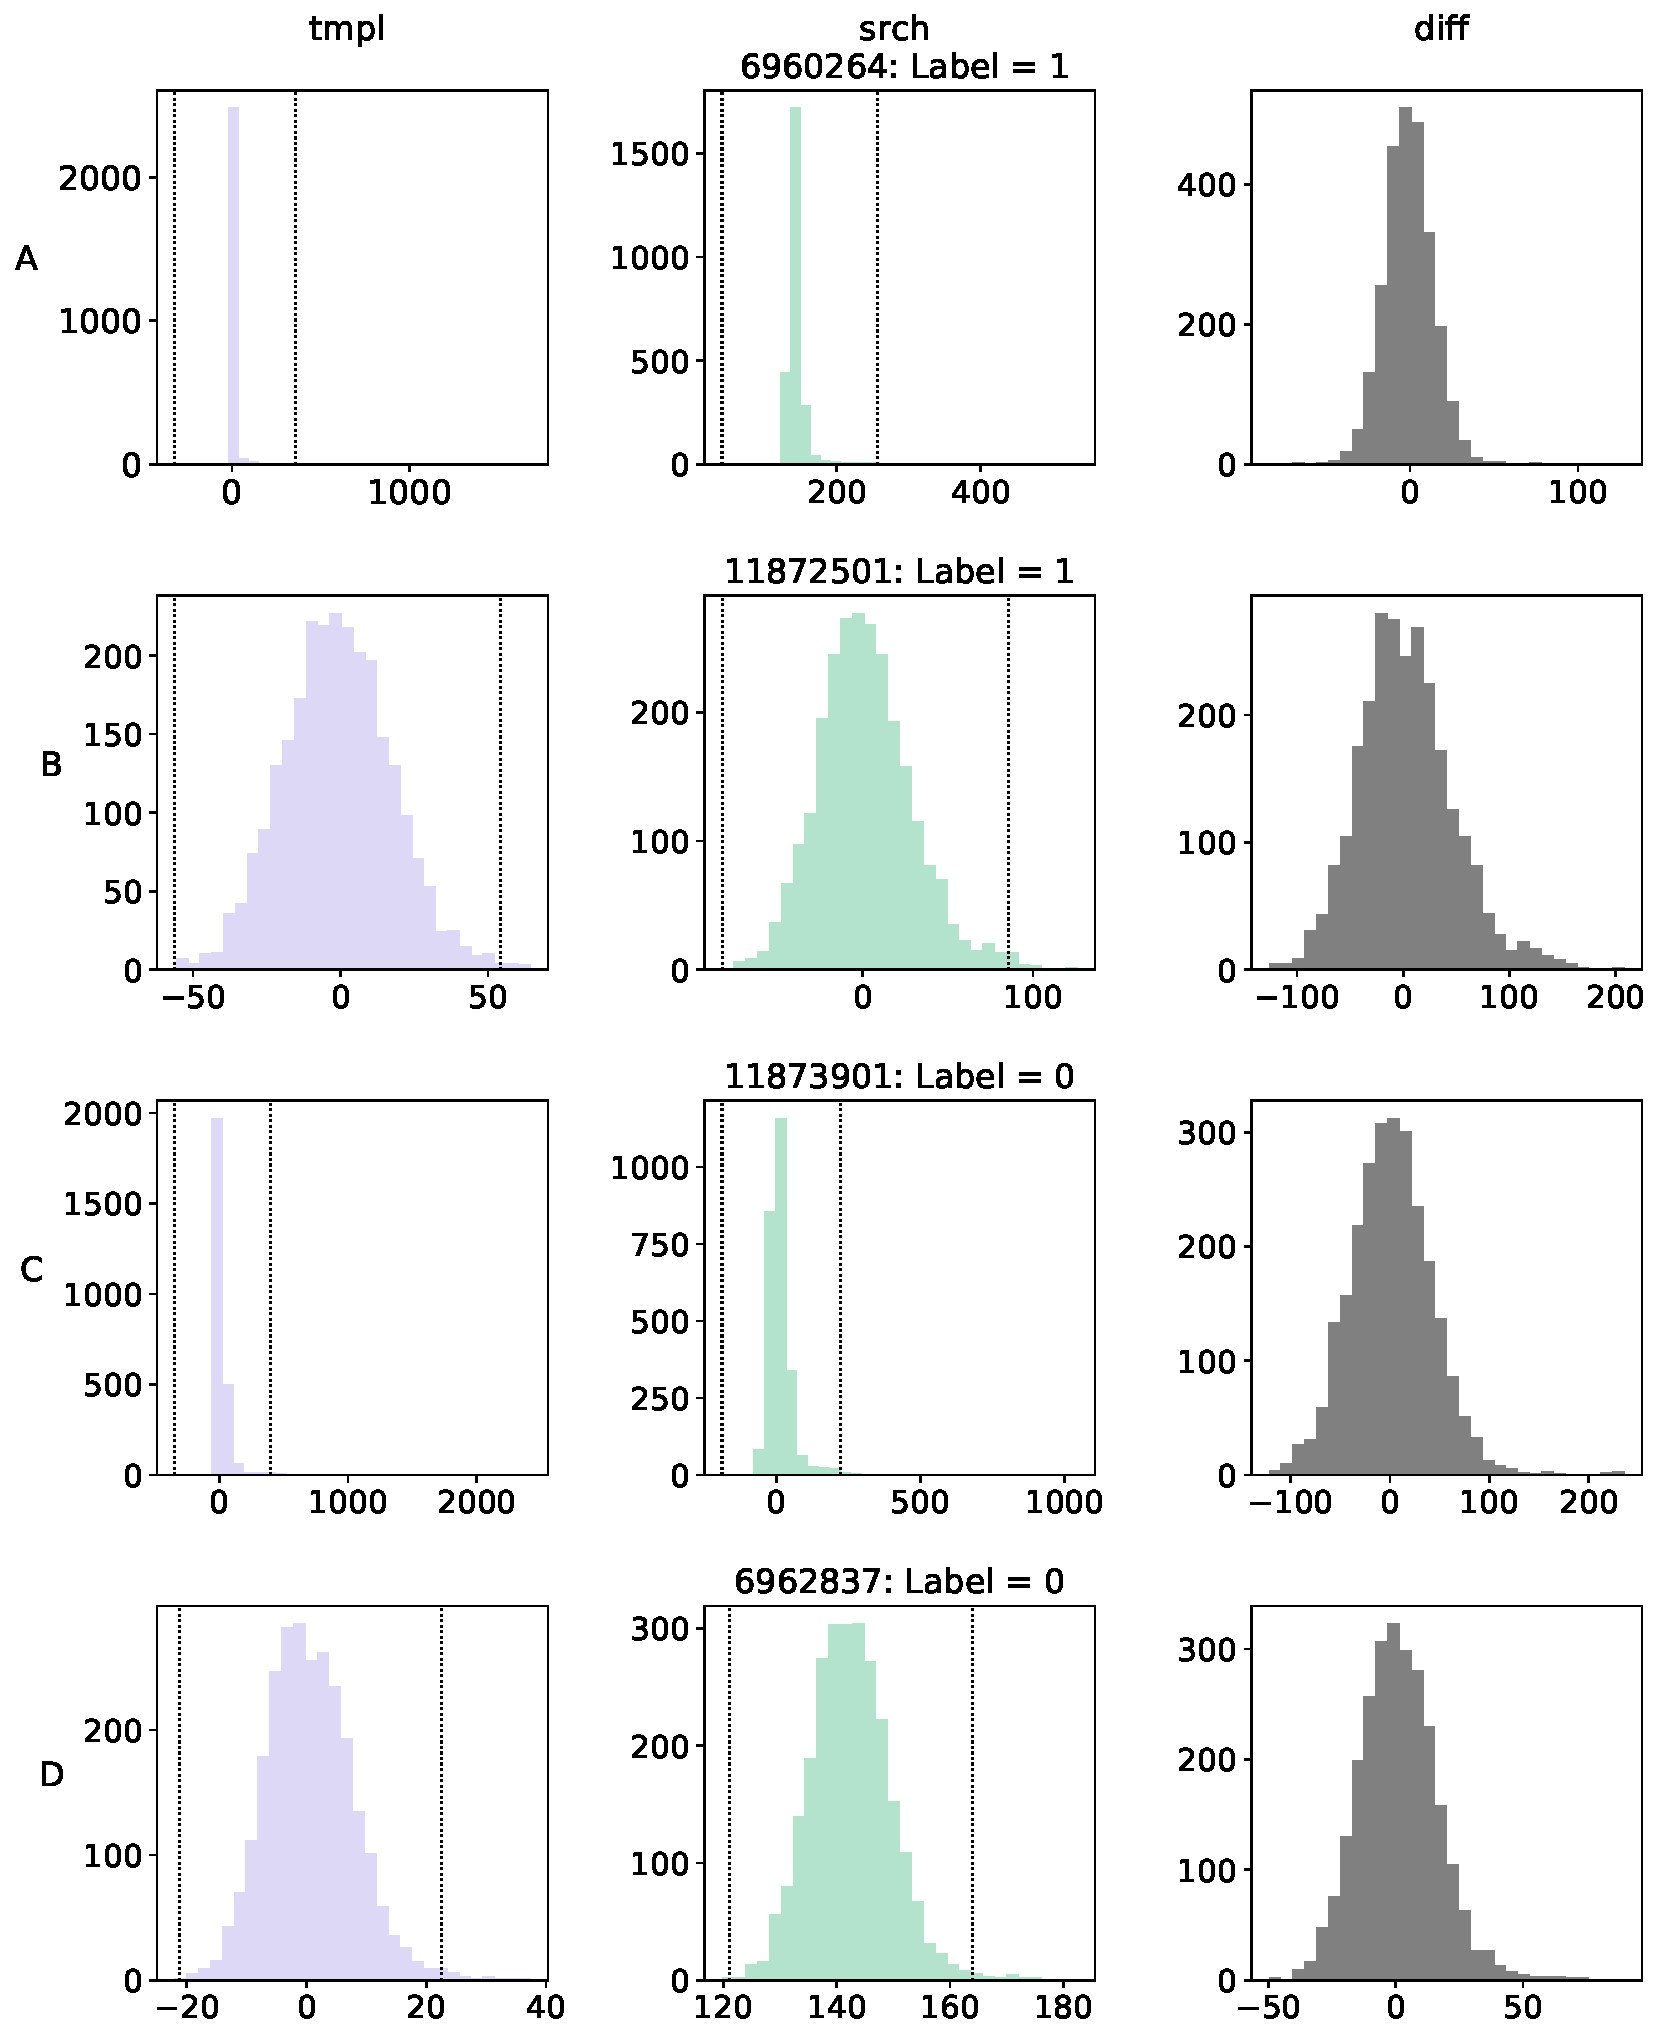
\includegraphics[width=0.6\linewidth]{
    figures/histnonorm_new_test_colors.pdf}
    \caption{Histogram of pixel values for %Quantitative representation of 
    the data shown in \autoref{fig:examples_no_normalization} (before scaling and normalization). 
    While all difference images (right) show bell-shaped distribution, the template and search image in both ``bogus'' and ``real'' sets have different behaviours. For example, B and D have similar pixel values distribution, however, B is ``bogus'' and D is ``real''. The vertical lines show the $\mu \pm 3\sigma$ interval for the \search\ and \temp\ images. The \diff\ images (last right column) are standardized individually to a mean of $0$ and a standard deviation of $1$. The \search\ and \temp\ are instead scaled, setting the pixel contained inside the 3$\sigma$ interval (vertical lines on the histograms) to the range 0-1. This allows to retain negative values or as well values above $1$ while keeping the core of the distributions to within a homogeneous range.
               }
    \label{fig:histobeforenormalizarion}
\end{figure*}


\begin{figure*}
    \centering
    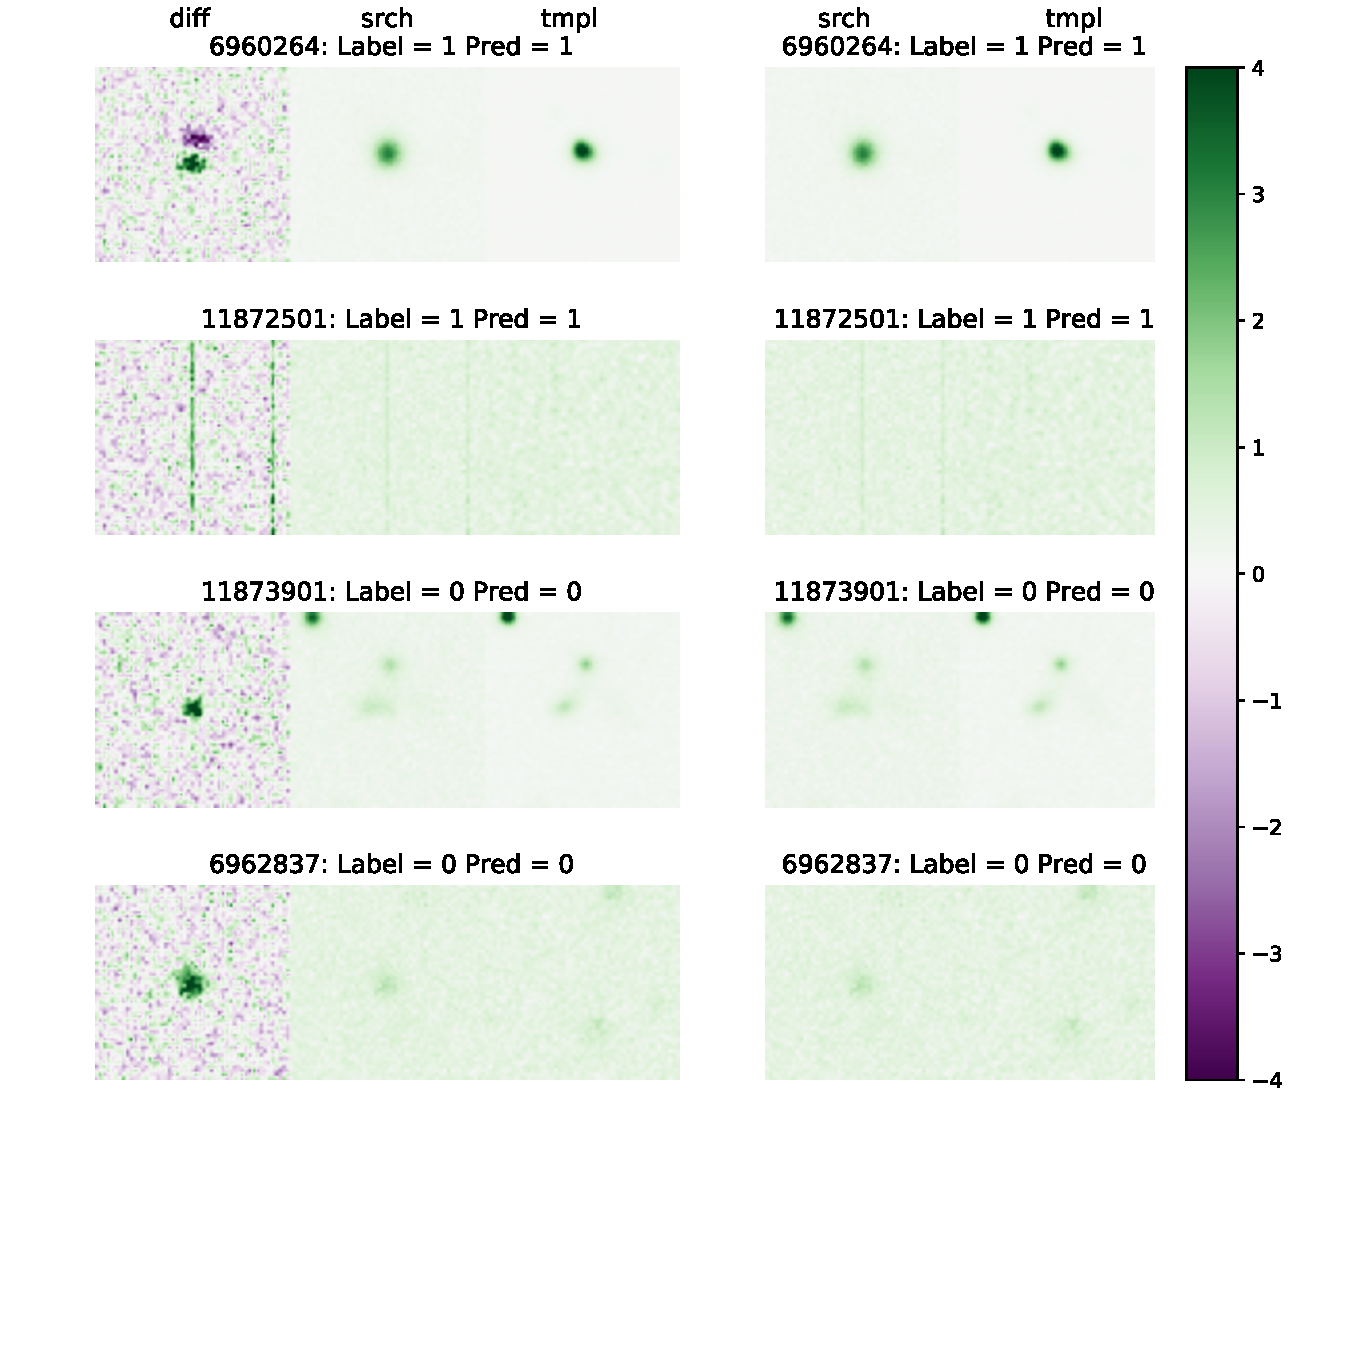
\includegraphics[width=0.7\linewidth]{
    figures/32dex_new_test.pdf}
    \caption{Horizontally stacked data for the examples shown in \autoref{fig:examples_no_normalization}. On the {\it left}, the composite images used as input to the \diabased\ CNN model: the composite follows the order, from left to right: \diff, \search, \temp. On the {\it right}, the composite images used for the \nodia\ model, composed of \search\ and \temp. Each images element was scaled or normalized following the description given in \autoref{sec:data} and \autoref{fig:histobeforenormalizarion} before combining them into a single image. Above each composite are the unique transient ``ID'', the original label, and prediction made by our model. The four transients were classified correctly by both \diabased\ and \nodia\ models. Purple shades indicate negative and green  positive pixel values.
%     \underline{Left}: Horizontally stacked normalized data for the examples shown in \autoref{fig:examples_no_normalization}. The stacked follow the order, from left to right: (\diff, \search, \temp). Each composite images is normalized as follows, the \diff\ are standarized (subtracting the mean and dividing by the standard deviation); \search\ and \temp\ are preprocessed using the min-max scheme. This is the format of the data input in the neural network (see section \ref{subsection: model_neural_network}).
% \underline{Right}: Horizontally stacked normalized data for the examples shown in \autoref{fig:examples_no_normalization}. The stacked follow the order, from left to right: (\search, \temp). Each composite images is normalized as follows, \search\ and \temp\ are preprocessed using the min-max scheme. This is the format of the data input in the neural network (see section \ref{subsection: model_neural_network}). The divergent color map used is \texttt{PRGn}, given by python
}
    %The color map used is ``viridis'', given by python. This images are the final data used for the Neural Network model.  }
    \label{fig:examples_hstack_normalization}
\end{figure*}


\section{state of the art and traditional solutions to detection of transients}\label{sec:stateofart}
\label{stateofart}
\subsection{Difference Imaging}
\label{sec:DI}
Difference images produced subtracting a template generated coadding multiple images \citep[\eg][]{Kessler_2015} from a sky image are currently the basis for most astrophysical transient search algorithms. The difference image allows brightness changes to be detected even if embedded in Galaxy light, for example, in the case of extra-galactic explosive transients. Great efforts have been made to improve the quality and effectiveness of the difference images. Although the name may suggest the process simply entails subtracting images from each other, the procedure is in fact riddled with complications because of the following reasons. First, the images used to build the template and the search images are taken principally within different atmospheric conditions \citep{Zackay_2017} generating variations in the quality of the images. The construction of a proper template is also a delicate task; typically templates are built by stacking tens of images taken under favourable sky conditions at different times. This improves the image quality but also mitigates issues related to variability in the astrophysical objects captured in the image \citep{Hambleton_2020}: one wants to capture each variable source at its representative brightness. Typically then, the template image is of higher quality than the search image, and it is degraded to match the search image PSF and scaled to match its brightness. Yet, the scaling and PSF may vary locally in the image plane, especially for images from large field of view synoptic surveys such as the 2.2 sq. degrees DES or $\sim10$ sq. degrees Rubin images. Finally it is important that the images are perfectly aligned, both in the creation of the template and in the subtraction process to create the difference image. This implies accounting for rotation as well as potentially different warping effects on the images and template. Once the PSF match and the alignment is done, it is possible to subtract the degraded template from the search images to obtain the difference image. To degrade the image quality of the template to match the search image, a convolution kernel that must be applied to the template needs to be determined \citep{Alard_1998},
\begin{eqnarray}
    \text{\temp}(x,y) \otimes \text{Kernel}(u,v) = \text{\search}(x,y),
\end{eqnarray}

\noindent 
where \temp\ is the high-quality image, the template image, \search is the one night image or search image and $\otimes$ is the convolutional operation. The arguments $x$ and $y$ represent the coordinates of matrix that compose the images; $u$ and $v$ the coordinates of the kernel matrix. 

To solve the computationally expensive problem of matching PSFs, the kernel can be decomposed in terms of simple functions, for instance Gaussian functions, and the method of least squares can be used to determine the best values for the kernel. The fitted solution of one search image can be determined in a short computational time. However, the computational cost scales with the image size and resolution. Surveys and telescopes constructed with the goal of discovering new transients are generally designed to collect tremendous amount of data to maximize event rate (detection of astrophysical transients).  For the DES, the computational cost per 2.2 sq. degree image $\sim 15.5$ CPU hours (with roughly 2/3 of that time spent on PSF matching).  The upcoming Rubin LSST will collect more than 500 images every night each with 3.2 Gigapixels. This process thus is bound to turn out to be very expensive.
In this paper, we trained our models on postage stamps where transients were detected or simulated (see \autoref{sec:data}), thus a direct comparison of the computational cost is not trivial. A detailed discussion of the computational cost of our models is included in \autoref{sec:computationcost} and the CPU Node hours required to train and generate predictions from our models are reported in \autoref{tab:acc results}. We note here that, with a Deep Neural Network approach to this problem, the computational cost is high in training, but the predictions are essentially instantaneous.

A bad subtraction can occur either because of poor PSF matching, poor alignment, or poor correction of image warping. In all of these cases, the subtraction would lead to artifacts or ``bogus'' alerts, like the one show in the difference image in  \autoref{fig:examples_no_normalization}A and B. In particular: in \autoref{fig:examples_no_normalization}A, the difference image shows a so-called ``dipole'', where one side of a suspected transient is dark and the other side bright: this typically arises in case of mis-alignments, but it might also be caused by moving objects in the field, or differential chromatic refraction \citep{carrascodavis2021alert}. Conversely, \autoref{fig:examples_no_normalization}B shows a ``bogus'' alert caused by an image artifact: a column of bad pixels in the search image. At this location there is no astrophysical object in the image thumbnail: no host galaxy or star that could give rise to variations.

Panels \autoref{fig:examples_no_normalization}C and \autoref{fig:examples_no_normalization}D show genuine transients in our DES training data: in both of these two examples, there is a clear transient in the \diff\  images (high pixel values at the center of the image).

\subsection{Autoscan and other feature-based Real Bogus models}
\label{sec:autoscan}

We developed our models on data collected in the first year of DES. Thus, a direct precursor of our work is \cite{Goldstein_2015}, in which the authors created an automated RB based on a Random Forest (RF) supervised learning model \citep{ho1995random} to detect transients, and particularly supernovae, in the DES data, hereafter refered to as \texttt{autoscan}. For these kinds of models, the process of selecting and engineering features is pivotal. %\citep{2011AAS...21720507S} (\masao{I suggest removing this reference}).
% \footnote{The data can be found at \url{https://portal.nersc.gov/project/dessn/autoscan/\#}} 
\texttt{Autoscan} is based on 38 features derived from the \diff, \search\ and \temp\ images. The selection and computation of these features was done attempting to represent quantitatively what humans would leverage in visual inspections. For instance, \texttt{r\_aper\_psf}  distinguishes a bad subtraction of \search\ and \temp\ that would lead to a \diff\ qualitative similar to  \autoref{fig:examples_no_normalization}A; the feature \texttt{diffsum} measures the significance of the detection by summing the pixel values in the center of the \diff\ image; the feature \texttt{colmeds}, indicating the CCD used for the detection, is designed to identify artifacts specific of a CCD, like bad rows/columns of pixels.


In other RB models, like in \cite{S_nchez_2019},
the feature selection is performed purely statistically: features were initially selected based on variance thresholds. In the same work, different techniques are explored to reduce the number of features, and thus the complexity of the classification problem. For example, a RF model was trained using all features. Then, feature values were randomly modified and the performance on the ``new'' data set was analyzed. Decreased accuracy associated to a change of a feature measured the importance of the feature that was modified. In this way the authors reduced the dimensionality of the problem by removing possible redundant or irrelevant information. Examples of models based on features closer to the data include \cite{Mong_2020}, where the features are simply the flux values of the pixels around the center of the image.




\subsection{AI approach}\label{sec:AI}


CNNs have demonstrated enormous potential in image analysis including object detection, recognition, and classification across domains \citep{5206848}. Examples of astrophysics applications of CNNs include \citet{Dieleman_2015} for galaxy morphology prediction, \citet{Kim_2016} for star-galaxy classification, \citet{PhysRevLett.120.141103} for signal/background separation for Gravitational Waves (GW) searches, where the GW time series are purposefully encoded as images to be analyzed by a CNN, and many more.


CNNs are particularly well-suited to learning discriminating features from image input data. CNNs can work on high dimensional spaces (here the dimensionality of the input is as large as the number of pixels in the image) due to the generalizability of the convolution operation to $n$ dimensions while preserving relative position information. Vectors of raw pixel values can theoretically be used to train traditionally feature-based models, such as RFs, but pixel-to-pixel position data in higher dimensions is unequivocally lost. Previous studies already compared feature-based supervised models, like RF, and supervised CNNs for RB, demonstrating that CNN generally leads to increased accuracy.  In \cite{Gieseke_2017} an accuracy of $\sim0.984$ is achieved with a RF model in the RB task, and it increases to $\sim0.990$ when applying a CNNs to the same data. In \cite{Cabrera_2016}  accuracy of $\sim 0.9889$ achieved with a RF is increased to to $\sim0.9932$ with a CNN. In \cite{Cabrera_Vives_2017}, an RF gave 0.9896 and a CNN 0.9945. In \citet{Liu_2019} the accuracy improves from $\sim0.9623$ with a RF to $\sim0.9948$ with a CNN.

Beyond RB, a model for image-based transient classification through CNNs has been prototyped by the Automatic Learning for the Rapid Classification of Events team \citep[ALeRCE][]{carrascodavis2021alert}. The model classifies between AGNs (Active Galactic Nuclei), SNe (SuperNovae), variable stars, asteroids, and artifacts in The Zwicky Transient Factory \citep[ZTF]{Bellm_2018} survey data with a reported accuracy exceeding 95\% for all types, except SNe (87\%). This CNN model was trained using a combination of the \search, \temp, and \diff.%, where rotational invariance was considered by training the model with rotated version of the images and features that characterize each astronomical object type were passed through a layer and concatenated with the output layer of the images. %They results have shown that AGN can be miss-classify for VS and vice versa; SN for asteroids or bogus; asteriods for SN or VS, and bogus for all of them except AGN.

The problem we propose to address here is exclusively the RB classification, but we explore the potential of leveraging AI to bypass the DIA step. 
Existing CNN RB models differ not only in their architecture (for example, a single or multiple sequences of convolutional, pooling, dropout, and dense layers) but also in the choice of input. For instance, \cite{Gieseke_2017} used the \temp, \search, and \diff\ images in combination for training their CNN; \cite{Cabrera_2016} augmented this image set with an image generated as the \diff\ divided by an estimate of the local noise;  \cite{Cabrera_Vives_2017} trained an ensemble of CNNs on different rotations of this four-fold image set. Conversely, \citet{Liu_2019} used the \diff\ as the sole input. Although, all these attempts have shown good results with accuracy higher than $90\%$, these models all rely on DIA to construct the \diff. Taking into account that \diff\ are built from the \temp\ and \search, and in principle, should carry no additional information content than the search-template pair alone, a logical step to follow would be to only consider the two latter images.  

A first attempt in this direction is presented in \cite{wardega2020detecting}. 
\cite{wardega2020detecting} trained a model that could distinguish between optical transient and artifacts using a search image from Dr. Cristina V. Torres Memorial Astronomical Observatory (CTMO, a facility of the University of Texas Rio Grande Valley\footnote{\url{https://www.utrgv.edu/physics/outreach/observatory/index.htm}}) and a template image from the Sloan Digital Sky Survey \citep[SDSS]{Gunn_2006}. They trained two Artificial Neural Network models, a CNN and a Dense Layer Network on simulated data and tested the models using data from CTMO and SDSS. The data used for training and testing had specific characteristics: transients were a combination of a source in the CTMO images (or \search\ image) and background in the SDSS image (or \temp\ image); artifacts were a combination of a source in both the CTMO and SDSS images. Within this dataset, both models yield high accuracy ($>95\%$) and establish a precedent for the possibility of avoiding the construction of the \diff\ to reliably detect optical transients. However, studies based on more diverse and realistic data, \eg, sources near galaxies, or embedded in clusters, are needed to demonstrate the feasibility of this approach. The data used in this paper fulfills this condition and is described in \autoref{sec:data}.


%\newpage
\section{Data} \label{sec:data}

This study is designed as a detailed comparison of CNN-based models, with and without \diff\ in input, with the results from one RB model, \texttt{autoscan} \citep{Goldstein_2015}. The choice of \texttt{autoscan} as our point of reference is motivated by its application to the discovery of transients in a state of the art facility, the Dark Energy Survey \citep{DES}, which can be considered a precursor of upcoming surveys like the Rubin Legacy Survey of Space and Time \citep{ivezic2019lsst}. The latter,  expected to start in 2024, will deliver $\sim 20~\mathrm{Tb}$ of high resolution sky image data each night, covering a footprint of $\sim20,000$ sq. deg. every $\sim 3$ nights, with expected millions of transients per night, demanding rapid methodological and technical advances in accuracy and efficacy of transient detection models.


%\section{
% The data used in this project consists of images collected by The Dark Energy Survey during its first observational season, August 2013 through February 2014. The data corresponds to observations of $898,963$ transients labeled by human inspection in two groups (\textit{OBJECT\_TYPE}): $454,092$ are labeled as real astrophysical transients ($1$) and $444,871$ as artifacts, or ``bogus'', as it is customary in the field,. Three images are made available for each transient, each of size $51 \times 51$, divided in three groups: the template (\temp) images, science images (\search) and the difference (\diff) images, correspond to the result of subtraction of template and science images [\cite{Goldstein_2015}]. Every group of three images (\diff,\search,\temp) correspond to a unique 'ID' and each one of the images has the same label information encoded in a binary 1 or 0 for ``real'' and ``bogus'' respectively.
% %}
% All the information about this training instances can be found in \url{https://portal.nersc.gov/project/dessn/autoscan/#}.\\




The data used in this work consists of postage stamps of images collected by the DES during its first observational season (Y1), August 2013 through February 2014\footnote{The data can be found in \url{https://portal.nersc.gov/project/dessn/autoscan/\#}} \citep{Abbott_2018}. The data corresponds to 898,963 DIA-sets, a template (\temp) image, search (\search) image, and their difference (\diff). The construction of the templates images for the DES Y1 leveraged the data collected in season two (Y2) as well as the Science Verification images (observations collected prior to survey start in order to evaluate the performance of the instrument). More information on the DES DIA pipeline can be found in \citep{Kessler_2015}.  Of these DIA sets, 454,092 contain simulated SNe Ia, which constitute the ``real'' astrophysical transients set (\texttt{label = 0}) and 444,871 are the actual data from DES, \ie, the ``bogus'' set (\texttt{label = 1}). Each image is offered in two formats: ``.gif'', and ``.fits''. The former is an 8-bit compressed format (convenient for visual inspection as it can be opened with commonly available software); the latter, the ``Flexible Image Transport System'', is a common data format for astronomical data sets which enables high precision with a large dynamic rage. The data in ``.fits'' format was used in this work.\footnote{More information related to how to manipulate this astronomical data format is available in \url{https://docs.astropy.org/en/stable/io/fits/}} Each image is $51 \times 51$ pixels - corresponding to approx 0.26 
arcseconds square of sky. 

 Some examples of the data are in \autoref{fig:examples_no_normalization}. Each transient is identified by a unique ``ID''. The metadata, includes the labels associated with each image as well as the the $38$ features used for classification in \citet{Goldstein_2015}.
 Because we only analyze postage stamps with detections, we implicitly still rely on the DIA to enable the detection step at this stage of our work. The \temp\ and \diff\ image in our postage stamps, however, are not PSF matched.
% \\
% \vspace{-10.8mm}


 %The other two columns corresponded to the ``ID'' and the ``OBJECT$\_$TYPE'': ``real'' (0) and ``bogus''(1); these two were used for this work.
\subsection{Scaling and normalization}\label{subsec:scaling}


A word about data preparation and normalization is in order as  astrophysical images are inherently very different from the images upon which CNNs have been built. When training CNN models for image analysis, each image is typically simply scaled to a common range ($0-1$). However, the dynamic range of an astrophysical image is typically large and the distribution of pixel values is generally very different from Gaussian, with the majority of pixels sitting at low values (the sky) and a few pixels at or near saturation (which in some cases may carry the majority of the information content). 
Furthermore, in the DIA-set case, the pixel-value distribution of the \diff\ differs qualitatively from the \temp\ and \search\ ones. While the \temp\ and \search\ are typically naturally positive valued with a long tail at the bright end (right-skewed because of the presence of bright astrophysical sources such as galaxies that host transients or stars that vary), the \diff\ image is, in absence of variable or transient sources, symmetric around 0.

%To gave more relevance to the 
The \diff\ images %and for their Gaussian behavior, as seen in \autoref{fig:histobeforenormalizarion} (first left column); each of them was
were standardized % The \diff\ images would 
to have a mean $\mu = 0$ and a standard deviation $\sigma = 1$. The \search\ and \temp\ images, instead, were scaled %minimum and maximum value for each image and considering pixel values inside the 
to map the $\mu\pm 3\sigma$ interval of the original image to $0-1$. %Meaning that $mean \pm 3\sigma$ would be $0$ or $1$ respectively. However, 
This scheme allows us to retain resolution in the shape of the core of the distribution while also retaining extreme pixel values. % allows  negative values and values above $1$ because extreme (outside the $3\sigma$ clip) values were scaled too. 
    \autoref{fig:histobeforenormalizarion} shows the distribution of pixel values for four DIA sets, for the same data as in \autoref{fig:examples_no_normalization}, which include two ``real'' and two ``bogus'' labels. \hyperref[sec:appendixa]{Appendix A} shows the pixel distributions before and after scaling for the same data.


% \begin{figure}[H]
%     \centering
%     \includegraphics[width=0.6\linewidth]{
%     figures/histnorm_new_test.pdf}
%     \caption{}
%     \label{fig:histoafternormalizarion}
% \end{figure}




% For the Neural Network Model, the first step was to horizontally stacked each image of each group (already normalized) per ``ID'', following the order (\diff, \search, \temp), and using \textit{np.concatentate}; the size of the data set is then (Number of transient to be considered, $51$, $153$). Some examples are in \autoref{fig:examples_hstack_normalization}. The second step was to have a balance (data set, in which the total of ``real'' (0) and the total of ``bogus'' (1) transient are equal or very similar.  
% \begin{figure}[H]
%     \centering
%     \includegraphics[width=0.4\linewidth]{
%     figures/3dex_new_test.pdf}
%     \caption{Horizontally stacked normalized data for the examples shown in \autoref{fig:examples_no_normalization}. The stacked follow the order, from left to right: (\diff, \search, \temp). Each composite images is normalized as follows, the \diff\ are standarized (subtracting the mean and dividing by the standard deviation); \search\ and \temp\ are preprocessed using the min-max scheme. This is the format of the data input in the neural network (see section \ref{subsection: model_neural_network}).
%     The divergent color map used is \texttt{PRGn}, given by python.} %This images are the final data used for the Neural Network model.  }
%     \label{fig:examples_hstack_normalization}
% \end{figure}

% The training and testing data set without \diff\ images were constructed based on the previous triplet and simply just cutting the \diff\ image.


% \begin{figure}[H]
%     \centering
%     \includegraphics[width=0.35\linewidth]{
%     figures/2dex_new_test.pdf}
%     \caption{Horizontally stacked normalized data for the examples shown in \autoref{fig:examples_no_normalization}. The stacked follow the order, from left to right: (\search, \temp). Each composite images is normalized as follows, \search\ and \temp\ are preprocessed using the min-max scheme. This is the format of the data input in the neural network (see section \ref{subsection: model_neural_network}). The divergent color map used is \texttt{PRGn}, given by python}
%     %The color map used is ``viridis'', given by python. This images are the final data used for the Neural Network model.  }
%     \label{fig:examples_hstack_2Dnormalization}
% \end{figure}


\begin{figure*}

   \centering
   \includegraphics[width=0.45\linewidth]{
    figures/aaa_big.pdf}
    \includegraphics[width=0.45\linewidth]{figures/ccc_bug.pdf}
   \caption{Architecture of the Neural Networks used in this project to classify ``real'' and ``bogus'' transients. {\it Left}: the \diabased\ model that uses image triplets as input (\diff, \temp, \search). The input layer is $51 \times 153$ (see left \autoref{fig:examples_hstack_normalization}); a convolution layer $(5\times 5)$ learns $16$ filters; max pooling $(2\times2)$ and dropout; convolution $(5\times 5)$ learns $32$ filters;  maximum pooling $(2\times2)$ and dropout; convolution $(5\times 5)$ learns $64$ filters;  maximum pooling $(2\times2)$ and dropout; flatten layer, Dense $(32)$ and the output is a Dense $(2)$-class layer. {\it Right}: the \nodia\ model that uses the \temp\ and \search\ images only. The input layer is $51 \times 102$ (see right \autoref{fig:examples_hstack_normalization}); a convolution layer $(7\times 7)$ learns $1$ filter; maximum pooling $(2\times2)$; convolution $(3\times 3)$ learns $16$ filters;  maximum pooling $(2\times2)$ and dropout; convolution $(3\times 3)$ learns $32$ filters;  maximum pooling $(2\times2)$ and dropout; flatten layer, Dense $(32)$ and the output was a Dense $(2)$-class layer.The illustrations were made using NN-SVG tool by \citet{LeNail2019}.}
\label{fig:architecturesCNN}
\end{figure*}


One further decision has to be made in combining the three images in the DIA set to feed them to the CNN. We stacked the scaled \diff, \search\ and \temp\ horizontally. %  the three each image (already standardized and scaled) per ``ID'', following the order (\diff, \search, \temp), and using \textit{np.concatentate}; 
Thus the size of the data in input to our CNN is ($N_{tr}\times51\times153$), where $N_{tr}$ is the number of transients to be considered. Four examples of the data ``triplets'' in input to our \diabased\ CNN are in the left panel of \autoref{fig:examples_hstack_normalization}. Following this horizontal structure, we mimic closely the way that human scanned this type of data for classification, and we will take advantage of this scheme when examining the models' decisions in \autoref{subsec: saliency}, although stacking the images along a third depth axis has also been tested, with no differences in the model accuracy.

But our goal is to test the performance of models that do not use the DIA. Thus for our \nodia\ models the training and testing data set were constructed in the same way as the previous triplets, but without the \diff\ image. Some examples are in the right panel of \autoref{fig:examples_hstack_normalization}.




% \onecolumngrid

% \newpage
\section{Methodology}\label{sec:method}



\subsection{Basics of Neural Networks}\label{subsection: intro_neural_network}
Neural Networks are models that learn important features and feature associations directly from data. % by training with a portion of the total data. 
These are typically supervised learning models used for classification or regression. They consist of a series of layers of linear combinations of the input data each with real value parameters known as weights and biases, combined with activation functions that enable learning {\it non-linear}, potentially very complex, relationships in the data. The weights tell us the relevance of the input feature with respect to the output, and the biases are the threshold value that determine the output. %(e.g. if a final output value is greater than a certain threshold then is A otherwise is B). 
Fitting these quantities to the data minimizes the %loss These quantities are the ones that guarantees the minimum
loss,
meaning the prediction is as close as possible to the original target/label \citep{nielsen_NN}. For Deep Neural Networks (DNNs), ``deep'' refers to the fact that there are multiple hidden layers, besides the input and output layer.  %that follow a layer structure, where each layer learns new and complex features of the data, architecture of these models usually consist on a input layer + hidden layers + output layer. Each hidden layer has weights and biases that is connected with the other hidden layers and both input and output data. 
With this architecture the features learned by each layer do not follow a human selection, rather, the features arise in the analysis of the data \citep{LeCun_Bengio_Hinton_2015}. Among DNNs, CNN models have layers that represent convolutional filters.
%The layers used in this work are:  \mintinline{c}/Conv2D/, \mintinline{c}/Dropout/, \mintinline{c}/Flatten/, \mintinline{c}/Dense/, etc... - a description of the structure and use of these standard layers can be found in 
More information on DNNs and CNNs can be found in \cite{DBLP:journals/corr/abs-1803-08375, 10.5555/2999134.2999257, Dieleman_2015}, as well as \cite{Gieseke_2017}, among many others.

We used the \texttt{Keras}\footnote{\url{https://keras.io/api/layers/convolution\_layers/convolution2d/}.} implementation of the CNN \citep{chollet2015keras}.




\subsection{DIA and noDIA based models architecture}


The input of our Neural Networks are the horizontally stacked images of size $51 \times 153$ for the \diabased\ model (\diff, \search, \temp), and $51 \times 102$ for \nodia\ model (\search, \temp). For both the \diabased\ model and the \nodia\ model $100,000$ images were used, $80,000$ images for training  and for validation and testing $20,000$ each. The images were selected randomly from the $898,963$ and while certainly training with a larger set can lead to higher accuracy, the amount of images was sufficient for this comparison of \diabased\ and \nodia\ models while being conservative with limited computational resource. The data is composed of $50,183$ images labeled as ``bogus'' and $49,817$ labeled as ``real''. %Each model was tested using $20,000$ divided as  $9922$ ``bogus'' and $10,078$ ``real''.\\

The network architectures used for this work are shown in  \autoref{fig:architecturesCNN}, left panel, for the \diabased\ model, and right  panel for the \nodia\ model. More details about the architecture can be found in \hyperref[sec:appendixb]{Appendix C}. Both architectures follow a similar structure. In designing the neural networks, we started with the \diabased\ model and developed an architecture that would match the performance of \citet{Goldstein_2015}.  With this model in hand, we created a \nodia\ with a similar structure in order to enable direct comparison and measure the effect of the change in the input data. 
We emphasize that in the development of our models we followed two general guidelines: 
\begin{enumerate}
\item We pushed the accuracy of the  \diabased\ CNN model to match the accuracy of \texttt{autoscan}. While a more exhaustive architectural exploration or a hyperparameter grid search may well lead to increased efficacy, matching the accuracy of \texttt{autoscan} (at 97\%) is sufficiently for our demonstration. We further note that this historical data set cannot be further validated (by, for example, assessing the recurrence of transients at a sky position to validate the {\it bogus} nature of a non-simulated detection) and it is subject to potential label inaccuracies that may compromise the ability to achieve a better performance. The final architecture used is one that reached the same accuracy as \citet{Goldstein_2015}, and  False Positive and False Negative Rates most similar to the ones obtain in \citet{Goldstein_2015}  (see \autoref{fig:confusiomatrix_models} and \autoref{sec:results}). Once we matched the \texttt{autoscan} performance, we focused on the potential for removing the \diff\ image from the input.
\item While the architecture of the \diabased\ CNN was designed with the attempt to achieve a specific target performance, the architecture of \nodia\ is deliberately kept as close as possible to that of the \diabased\ model. This enables a direct comparison of the effects of the removal of the \diff\ image. 
In other words, the hyperparameters and architecture of \nodia, shown on the right in \autoref{fig:architecturesCNN} were not optimized explicitly for RB classification, rather we chose a standard architecture, only modifying the original design to adapt for the different dimensionality of the input data. One further deliberate modification is implemented in the choice of a single-filter first layer for \nodia. The CNN that is not offered the \diff\ image needs to learn the image PSF, which is constant across the postage stamp-size image, and can be modeled with a single filter. 
\end{enumerate}

\tatiana{A grid search was implemented in the \nodia\ model, varying the kernel size of the three convolutional layers 1, 3 and 6 and the batch size. %The combination tested and their respective performances are given in APPENDIX. 
No better combination of hyperparameters was found.  }

\tatiana{As part of the optimization tasks, pre-made deep learning models available in \texttt{Keras} were trained with the data of the \diabased\ case presented here. VGG16 \citep{VGG16} was implemented, while the model has a similar performance in terms of accuracy and other metrics, presented overfitting after ~50 epochs. ResNet 50-V2 \citep{RESNET50V2} was also implemented, overfitting was presented during all training process. Pre-made architecture limit the size of the images used for train the model. To implement these architectures the data must have the form of: (height, width, 3). In consequence the selection that we made in this work to horizontally stacked the images is not longer possible, also training the model with the \nodia\ approach is only possible by changing the shape of the images to match the require third depth axis. In such a case we will loss the spatial and geometrical information of the data.   }


\subsection{Saliency maps}\label{subsec: saliency}


% \masao{This is a very interesting section!  For readers like me who don't know much about how saliency maps are produced, can you write a couple of sentences about how they are made?  I think you said something about removing each pixel and looking at how much the predictions change.  A short description is helpful for the uneducated reader like me.}

Saliency maps quantify the importance of each pixel of an image in input to a CNN in the training process. They provide some level of interpretability through a process akin to feature importance analysis by enabling  an assessment of which are the pixels the model relies on the most for the final classification. If the task were, for example, to identify cats and dogs in images, the expectation will be to find that the most important pixels are located within the the dog or cat bodies, and not in the surrounding, while if the task were to identify activities performed by cats and dogs, one may find the important pixels both within the dogs and in the surrounding, particularly in objects associated with the performed tasks. Furthermore, some portion of the subject's body may be most distinctive (ears, nose) and we would expect more importance being given to those pixels. The "importance": of a pixel would be simply measured by the weight the trained NN assigns to that pixel in the case of a single-layer perceptron, but in the case of Deep Neural Networks, a highly non-linear operation is performed on the input data, and the importance, or saliency, of an input feature, or pixel, is harder to assess. We follow \citep{simonyan2014deep}'s definition of saliency: denoting the class score with $S_c$, such that the NN output on image $\mathcal{I}$ is represented by $S_c(\mathcal{I})$, the saliency map is given by :
\begin{eqnarray}
 S_c(\mathcal{I}) \approx w^T \mathcal{I} + b,\\
 w = \frac{\partial S_c}{\partial \mathcal{I}} \biggr\rvert_{\mathcal{I}_0}.
 \end{eqnarray}
 
That is: $w^T$ is the weight and $b$ the bias of the model. $w$ is the derivative of $S_c$ with respect to $\mathcal{I}$ calculated specifically in the local neighborhood of pixel $\mathcal{I}_0$, and the approximation sign indicates a first order Taylor expansion has been used to approximate the solution.
The interpretation of the decision making by the CNNs have been studying as a tool for improving the efficiency of the performance of the CNNs, as done by \citep{DBLP:journals/corr/abs-2105-00937}. \tatiana{Within the transient detection approach, previous works, \eg\  \cite{Reyes_2018}, have implemented Saliency maps to detect the relevant pixels and improve perfomance on transient classification. }


\begin{figure*}
    \centering
    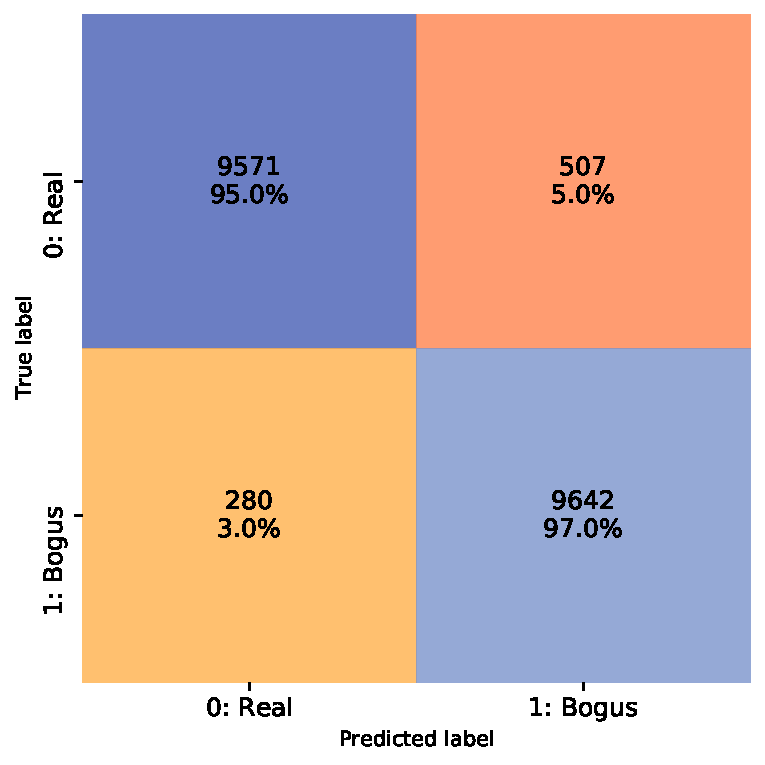
\includegraphics[width=0.45\linewidth]{
    figures/confusionmatrix_model_100K20KNERSCstam0-9CCCC_3s3DH.pdf}
    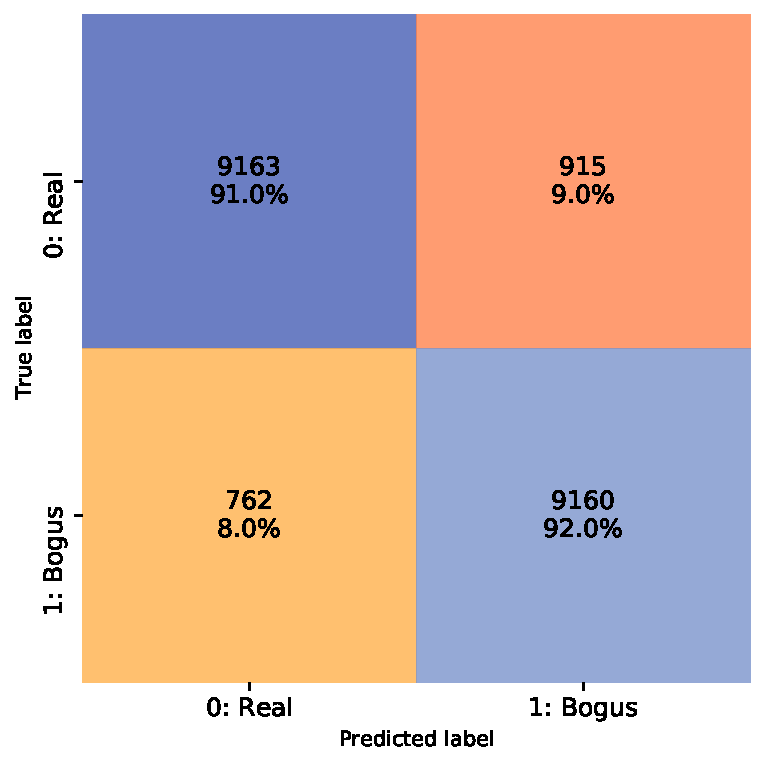
\includegraphics[width=0.45\linewidth]{
    figures/confusionmatrix_model_100K20KNERSCstam0-9CCCC_3s2DH.pdf}
    \caption{Confusion matrix (CM) for our testing data, a set composed of $10,078$ objects labeled as ``real'' and $9,922$ as ``bogus''.  Squares of the matrix, from the top left in the clockwise direction, indicate: True Positive (TP, \texttt{label = 0}, \texttt{prediction = 0} ), False Negative (FN, \texttt{label = 0}, \texttt{prediction = 1}), True Negatives (TN, \texttt{label = 1}, \texttt{prediction = 1}), and False Positive (FP, \texttt{label = 1}, \texttt{prediction = 0}). We note that here, somewhat unusually, 0 corresponds to ``real'' and ``positive'', and 1 to ``bogus'' and ``negative'', as we chose to remain consistent with the original labeling of the data presented in \citep{Goldstein_2015}. 
    {\it Left}: The CM of our \textbf{\diabased } model shows that from the $10,078$ transients labeled as ``real'', $9,571$ (\ie, 95\%) were correctly classified and the accuracy for the TN objects is even higher, at $97\%$. {\it Right}: The CM for the \nodia\ model shows that of the $10,078$ transients labeled as ``real'', $9,163$ (\ie, 91\%) were predicted correctly and the TN accuracy is $92\%$. }
    \label{fig:confusiomatrix_models}
% \end{figure}
\end{figure*}


\begin{figure}
    \centering
    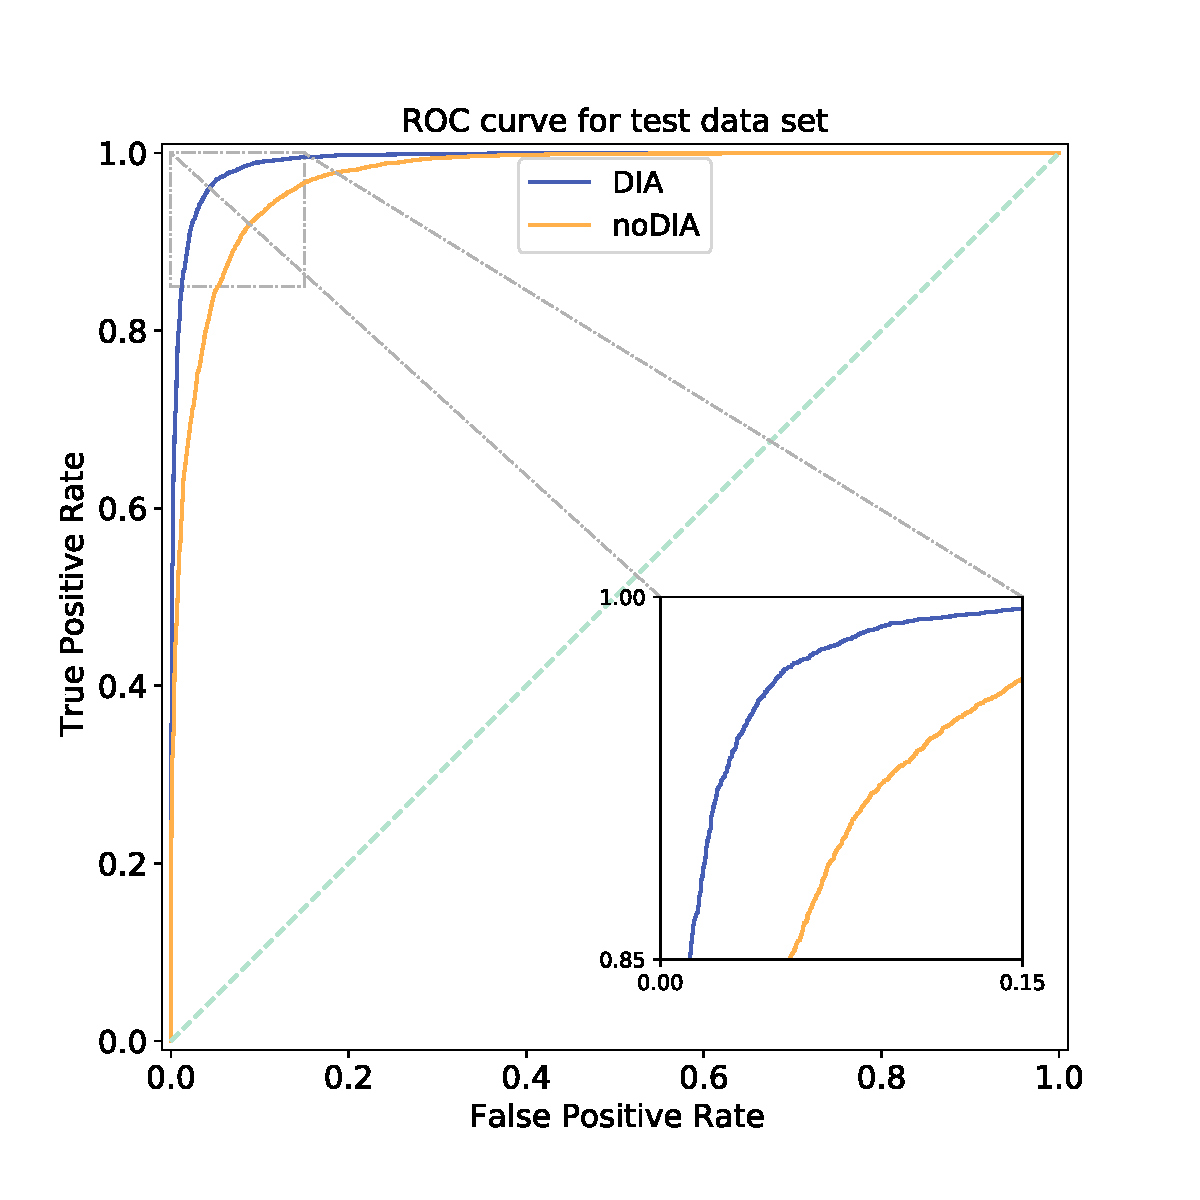
\includegraphics[width=1\linewidth]{
    figures/ROC_zoom.pdf}
    \caption{ROC curve for the $20,000$ images used for testing, Blue line for the  \diabased\ model, the area under the curve is $0.992$. Orange line, for the \nodia\ model, the area under the curve is $0.973$. This figure is discussed in \autoref{sec:results}.}
    \label{fig:roc_models}
\end{figure}

\begin{figure*}
    \centering
    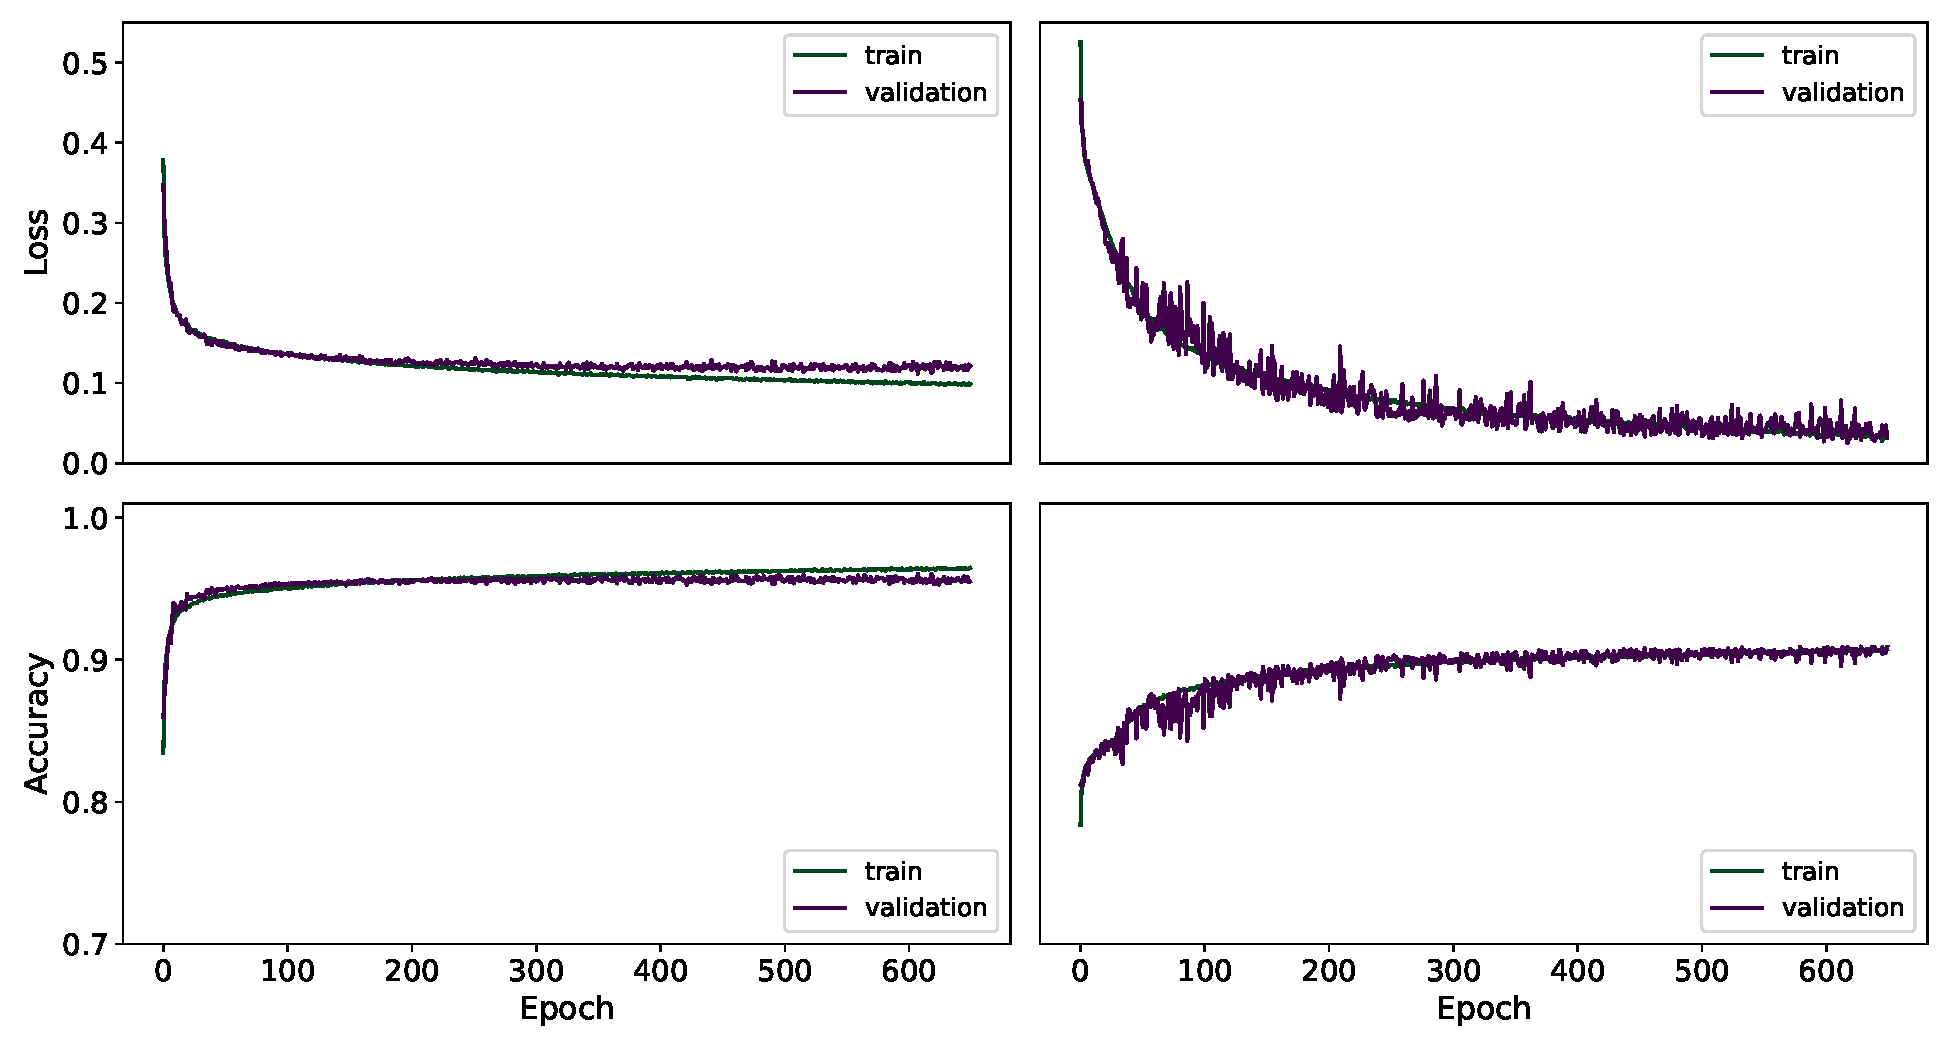
\includegraphics[width=0.9\linewidth]{
    figures/losscc.pdf}
    % \includegraphics[width=0.49\linewidth]{
    % figures/lossacc_modeloverleafCCC_scale(1).pdf}
    \caption{Loss (top) and accuracy (bottom) for both models presented in this work. Purple lines correspond to the validation data (20\% or 20,000 images) and green to the training data (80\% or 80,000 images). {\it Left}:  results for our \diabased\ model  (\autoref{fig:architecturesCNN}). {\it Right}: results for the \nodia\ model (\autoref{fig:architecturesCNN}). %This figure is discussed in \autoref{sec:results}.
    }
    \label{fig:loss_models}
% \end{figure}
\end{figure*}
Each pixel in an image in the training set is associated with the corresponding pixel in the saliency map, and the saliency score (the importance) of that pixel measures the change in model output as a function of changes in the value of that input pixel by back-propagation. The higher the value of a pixel in a saliency map, the more influence that pixel has in the final classification. In this work we also refer to these maps as maps of pixel importance. 


In our case, given the side-by-side organization of the three elements of the input image set, %(\diff, \search, \temp), 
the saliency maps can help us assess how much the \diabased\ model relied on the \diff\ to enable correct classification, and, thus, provide some intuition in the difficulty of the challenge offered to the \nodia\ model. 


For the \diabased\ model we have an expectation guided by intuition: that a greater concentration of important pixels should be found in the \diff\ image. In \autoref{sec:results},  we will consider the veracity of this hypothesis both qualitatively by visually inspecting the saliency maps, and by designing a saliency-based metric that enables a quantitative approach. We calculated the normalized sum of the saliency pixel values for each third of the image-triplet, corresponding to \diff, \search, \temp:

\begin{eqnarray}
\begin{split}
\idiff=\frac{\sum_{p_d}{s_{p_d}}} {\sum_{p}{s_p}};\\
\isearch=\frac{\sum_{p_s}{s_{p_s}}} {\sum_{p}{s_p}};\\
\itempl=\frac{\sum_{p_t}{s_{p_t}}} {\sum_{p}{s_p}};
\label{eq: saliencymetric}
\end{split}
\end{eqnarray} 
where $I$ indicated the importance of a segment of the input image, $p$ is an index running over all pixels and $s_p$ indicates the value of pixel $p$ in the saliency map. The denominator normalizes each metric by the total sum of the saliency pixel values. In the numerators, $p_d$ denotes the pixels in the leftmost third of the image, corresponding to \diff; $p_s$ the middle third corresponding to the \search; and $p_t$ the right most third, corresponding to the \temp. 
This metric allows us to assess the relative importance of the \diff\ (\search\ or \temp) component of the image in performing RB classification. Results from these metrics are discussed in detail in \autoref{subsec:results_seliancy}.\\

% This study is reproducible and all the code that supports the analysis presented here is available on a dedicated \texttt{GitHub} repository. \footnote{\url{https://github.com/taceroc/DIA_noDIA}.}



%\begin{figure*}
%\begin{tabular}
%\begin{minipage}[b]{0.45\linewidth}
%%\begin{figure}[t!]
%    \centering
%    \includegraphics[width=0.8\linewidth]{
%    figures/aaa_big.pdf}
%    \caption{Architecture of the Neural Network used in this project to classify ``real'' and ``bogus'' transients from the image triplet \textbf{(\diabased\ model)}. The input layer was $51 \times 153$ (see left \autoref{fig:examples_hstack_normalization}); a convolution layer $(5\times 5)$ learned $16$ filters; max pooling $(2\times2)$ and dropout; convolution $(5\times 5)$ learned $32$ filters;  maximum pooling $(2\times2)$ and dropout; convolution $(5\times 5)$ learned $64$ filters;  maximum pooling $(2\times2)$ and dropout; flatten layer, Dense $(32)$ and the output was a Dense $(2)$-class layer. The illustration was made using NN-SVG tool by \cite{LeNail2019}.}
%    \label{fig:architecture_NN}
%\end{minipage}
%\begin{minipage}[b]{.45\textwidth}
%%\begin{figure}[t!]
%    \centering
%    \includegraphics[width=0.8\linewidth]{
%    figures/ccc_bug.pdf}
%    \caption{Architecture of the Neural Network used in this project to classify ``real'' and ``bogus'' transients from the image duplex \textbf{(\nodia\ model)}. The input layer was $51 \times 102$ (see right \autoref{fig:examples_hstack_normalization}); a convolution layer $(7\times 7)$ learned $1$ filter; maximum pooling $(2\times2)$; convolution $(3\times 3)$ learned $16$ filters;  maximum pooling $(2\times2)$ and dropout; convolution $(3\times 3)$ learned $32$ filters;  maximum pooling $(2\times2)$ and dropout; flatten layer, Dense $(32)$ and the output was a Dense $(2)$-class layer.
        %\footnotetext{$\dag$ 
%        {The illustration was made using NN-SVG tool by \cite{LeNail2019}.}
%        }
%    \label{fig:architecture_2DNN}
    
%\end{minipage}
%\end{tabular}{cc}
%\end{figure*}

% \begin{figure}[hbt!]
%     \centering
%     \includegraphics[width=0.9\linewidth]{
%     figures/CNN.pdf}
%     \caption{Architecture of the Neural Network used in this project to classify ``real'' and ````bogus'''' transients from the image triplet. The input layer is $51 \times 153$ (see \autoref{fig:examples_hstack_normalization}; a convolution layer $(5\times 5)$ learns $16$ filters; maximum pooling $(2\times2)$; convolution $(5\times 5)$ learns $32$ filters;  maximum pooling $(2\times2)$; flatten layer, Dense $(32)$ and the output is a Dense $(2)$-class layer.}
%     \label{fig:architecture_NN}
% \end{figure}




% The first convolutional layer of this model, intends to recover the PSF (Point Spread Function) of the 
% \begin{itemize}
% \item \mintinline{c}/Conv2D/:\\

% According to the documentation of Convolutional layers in \url{https://keras.io/api/layers/convolution\_layers/convolution2d/}. The first parameter (\mintinline{c}/filter = 16 or 32 /) refers to the number of filters that the layer is going to learn. The outer layers learn less from the data than the inner layers. The second parameter (\mintinline{c}/kernel_size = (5,5)/) refers to the width and height of the filter that is multiplying the input data, the elements of the filter are the weights. The third parameter (\mintinline{c}/padding = "valid"/) define the way that the filter is going to sweep the input data, \mintinline{c}/"valid"/ refers that the operation between filter and input data is possible only if all the elements of the filters have a corresponding element in the input data. With this parameter the size of the output data is going to be smaller than the input. The latter parameters used here is the \mintinline{c}/activation = "relu"/, ``Rectified Linear Unit''. The output data, know as feature map, is pass through the activation function to get the bias. The \mintinline{c}/"relu"/ function is defined as:
% \begin{equation*}
% ReLU = 
% \begin{cases}
%     0, & x\le0\\
%     x, & x>0
% \end{cases}
% \end{equation*}
% The ReLU is an efficient activation function that improves the performance of the Neural Network. [\cite{DBLP:journals/corr/abs-1803-08375, 10.5555/2999134.2999257}]

% \item \mintinline{c}/MaxPooling2D/:\\
% Reduces the size of the output given in \mintinline{c}/Conv2D/ by a factor of $2$, selecting maximums values.

% \item \mintinline{c}/Flatten/:\\
% Reduces the dimensions of the data to be a one dimension array.

% \item \mintinline{c}/Dense/:
% Make the previous layer all fully connected with the next layer.\\
% \end{itemize}






% %A optimizer, loss and metric:
% \begin{minted}{python}
% opt = keras.optimizers.SGD(learning_rate=0.01)
% model.compile(optimizer=opt, loss="sparse_categorical_crossentropy", metrics=["accuracy"])
% \end{minted}

% The model is fit to the training data and this is split to have a validation set. We use \mintinline{c}/epochs=50, batch_size=20/.
% %and fitting the model as:
% \begin{minted}{python}
% history = model.fit(feat_tr2, targ_tr, validation_split=0.20, epochs=50, batch_size=20)
% \end{minted}

% The training data is divided into groups of $20$ elements. The weights of the model are updated after each group of $20$ is been fitted. After the $1$st epoch, the weights have been updating the numbers of groups of $20$ that exist.\\


% \newpage
\section{Results}\label{sec:results}
% \subsection{Neural Network}


The accuracies of our models %the model for DIA and no\diabased\  using the $80,000$ for training and the $20,000$ for testing 
are presented in \autoref{tab:acc results}. The \diabased\ model reached, by design, the accuracy of our benchmark model \texttt{autoscan}: ~97\% on True Negative (TN) rate and 95\% on True Positive (TP) rate (see \autoref{sec:method}). We remind the reader that we use the \texttt{autoscan} convention for the definition of TN and TP: Positive is a ``real'' transient ($\texttt{label = 0}$), negative is a ``bogus'' ($\texttt{label = 1}$). There is a drop of $\sim 4\%$ between the accuracy of the \diabased\ and the \nodia\ models. Along with the accuracy, in \autoref{tab:acc results} we present computational costs of training on 20,000 images measured in CPU Node hours,\footnote{The computational cost was calculated by using the formula given in \url{https://docs.nersc.gov/jobs/policy/} and the allocations information given by the system Iris \url{https://iris.nersc.gov}. Training time is reported in CPU hours. Prediction time is reported per “postage stamp” (1ms) and the classification operation is trivially parallelizable (can be run independently on each postage stamp).} and the clock time for the prediction for one single image.

\begin{table}
\footnotesize{
    \centering
    \begin{tabular}{|c|c|c|c|c|}
    \hline
    \multirow{2}{*}{\bf{Model}}& \multicolumn{2}{c|}{\centering \bf{Accuracy}}
 & \bf{Train time}$^7$ & \bf{Prediction}$^7$\\
    \bf{ }&\bf{Train} & \bf{  Test} & \bf{(CPU hours)} & \bf{(Clock-time, ms)}\\
    \hline
       \multirow{2}{*}{ \diabased}&\multirow{2}{*}{0.965}&$0.961\pm$&\multirow{2}{*}{$\sim$35}&\multirow{2}{*}{$1.00\pm0.03$}\\&&$0.004$&&\\ \hline
      \multirow{2}{*}{ \nodia}&\multirow{2}{*}{0.920}&$0.916\pm$&\multirow{2}{*}{$\sim$56}&\multirow{2}{*}{$0.30\pm0.01$}\\&&$0.007$&&\\ \hline
    \end{tabular}
    \caption{Comparative table of the accuracy and computational cost for both training and testing (different from validation) data for the \diabased\  (\autoref{fig:architecturesCNN}, left) and \nodia\  (\autoref{fig:architecturesCNN}, right) models. }
    \label{tab:acc results}}
\end{table}
% The accuracy of the model for \diabased\  input data for training and testing data was respectively: \mintinline{c}/Training accuracy: 0.9620/
% \mintinline{c}/Testing accuracy: 0.9590/. The accuracy of the model for no\diabased\  input data for training and testing data was respectively: \mintinline{c}/Training accuracy: 0.9147/
% \mintinline{c}/Testing accuracy: 0.9155/. 
% Using the $80,000$ for training and the $20,000$ for testing. \autoref{fig:loss_modelAAAD} and \autoref{fig:loss_modelCCC} show the loss and the accuracy through the epochs for the \diabased\  model (\autoref{fig:architecture_NN}) and no\diabased\  model (\autoref{fig:architecture_2DNN}) respectively.





% \begin{figure*}
% \begin{minipage}[b]{0.45\linewidth}
%     \centering
%     \includegraphics[width=1\linewidth]{
%     figures/lossacc_modeloverleaf_scale(1).pdf}
%     \caption{\textbf{\diabased\ } loss (top) and accuracy (bottom) for the model described in left \autoref{fig:architecturesCNN}. Purple line represent the validation data (20\% or 20,000 images) and the green the training data (80\% or 80,000 images).}
%     \label{fig:loss_modelAAAD}
% % \end{figure}
% \end{minipage}
% \begin{minipage}[b]{0.45\linewidth}
%     \centering
%     \includegraphics[width=1\linewidth]{
%     figures/lossacc_modeloverleafCCC_scale(1).pdf}
%     \caption{\textbf{\nodia\ } loss (top) and accuracy (bottom) for the model described in right \autoref{fig:architecturesCNN}. Purple line represent the validation data (20\% or 20,000 images) and the green the training data (80\% or 80,000 images).}
%     \label{fig:loss_modelCCC}
%     \end{minipage}
% \end{figure*}


% \begin{minted}{python}
% Training accuracy: 0.9892
% Testing accuracy: 0.9726
% \end{minted}

% The accuracy and loss plot for training and validation data:
% \begin{figure}[hbt!]
%     \centering
% \begin{minipage}{.4\textwidth}
% \centering
%     \includegraphics[width=1\linewidth]{
%     figures/lossacc_modelAAAD_3s\diabased\ H.pdf}
% %    \caption{Accuracy from training and testing data from the initial model.}
%     %\label{fig:accuracyinitialmodel}
% \end{minipage}%
% \begin{minipage}{.4\textwidth}
% \centering
%     \includegraphics[width=1\linewidth]{
%     figures/lossacc_modelCCC_3s2DH.pdf}
%     %\caption{Loss from training and testing data from the initial model.}
%     \label{fig:lossinitialmodel}
%     \end{minipage}%
%     \label{fig:acclossinitialmodel}
%     \caption{Accuracy and loss from the training and validation data for a set of composed by $1106$ transients, $555$ labeled as ``real'' and $551$ as ``bogus''. The data is evaluated in the Neural Network model.}
% \end{figure}



Confusion matrices for the testing set are shown for the \diabased\ model in left panel of  \autoref{fig:confusiomatrix_models} and for the \nodia\ model in the right panel of the same figure. In this figure, as in the following confusion matrices and histograms that we will present in \autoref{subsec:results_seliancy}, correct predictions are indicated in shades of blue, incorrect in shades of orange, and darker shades are associated with the true labels. The percent accuracy for each class, True Positives (TP), True Negatives (TN), False Positives (FP), and False Negatives (FN), as well as the number of images in each class are reported within the figure.  



The Receiver Operating Characteristic (ROC) curve shows the relation between the True Positive Rate (TP / (TP + FN)) also know as recall, and the False Positive Rate (FP / (FP + TN)) when changing the threshold value (\eg, a threshold of 0.5 will indicated that values greater than 0.5 would be classified as ``bogus''). The ROC for the testing data for the \diabased\ and \nodia\ models are presented in \autoref{fig:roc_models}. The Area Under the Curve (AUC), which can be used as a comprehensive metric of the aggregated classification performance of a model \citep{hanley1983method, hernandez2012unified}, is 0.992 and 0.973 for the \diabased\  and \nodia\ models respectively, demonstrating good performance for both models \tatiana{and within \texttt{autoscan} performance}.


The loss and the accuracy curves in the left panel of \autoref{fig:loss_models} for the \diabased\  model shows some evidence of overfitting (the validation curve flattens compared to the training curve) starting just a few epochs before training came to end of the 350-epochs; meanwhile, for the \nodia\ model in right \autoref{fig:loss_models}, after $650$ epochs there was no visual evidence of overfitting indicating that the model is still learning generalized information from the data; yet the accuracy improvements from epoch $350$ to $650$ were small.

The nature of the \nodia\ model leads to hypothesize that because the input data contains less information, this model takes longer to learn features from the data to be able to classify them. The \nodia\ model took in fact longer (more epochs) to come to stable accuracy and loss values. The loss and accuracy curves are also noisier for the validation of the \nodia\ model in right \autoref{fig:loss_models} compared to the \diabased\ model. This also can be explained with the same argument: the \nodia\ model had a harder problem to solve and its learning is less linear. We cannot however rule out, and in fact we suspect, that the hyperparameters or the architecture selected for the \nodia\ CNN model could be improved --- as this is a proof of concept paper and the architecture was chosen to enable a direct comparison with the \diabased\ model, future work will include experimenting with different architectures and an extensive grid-search to optimize hyperparameters.
\begin{figure*}
    \centering
    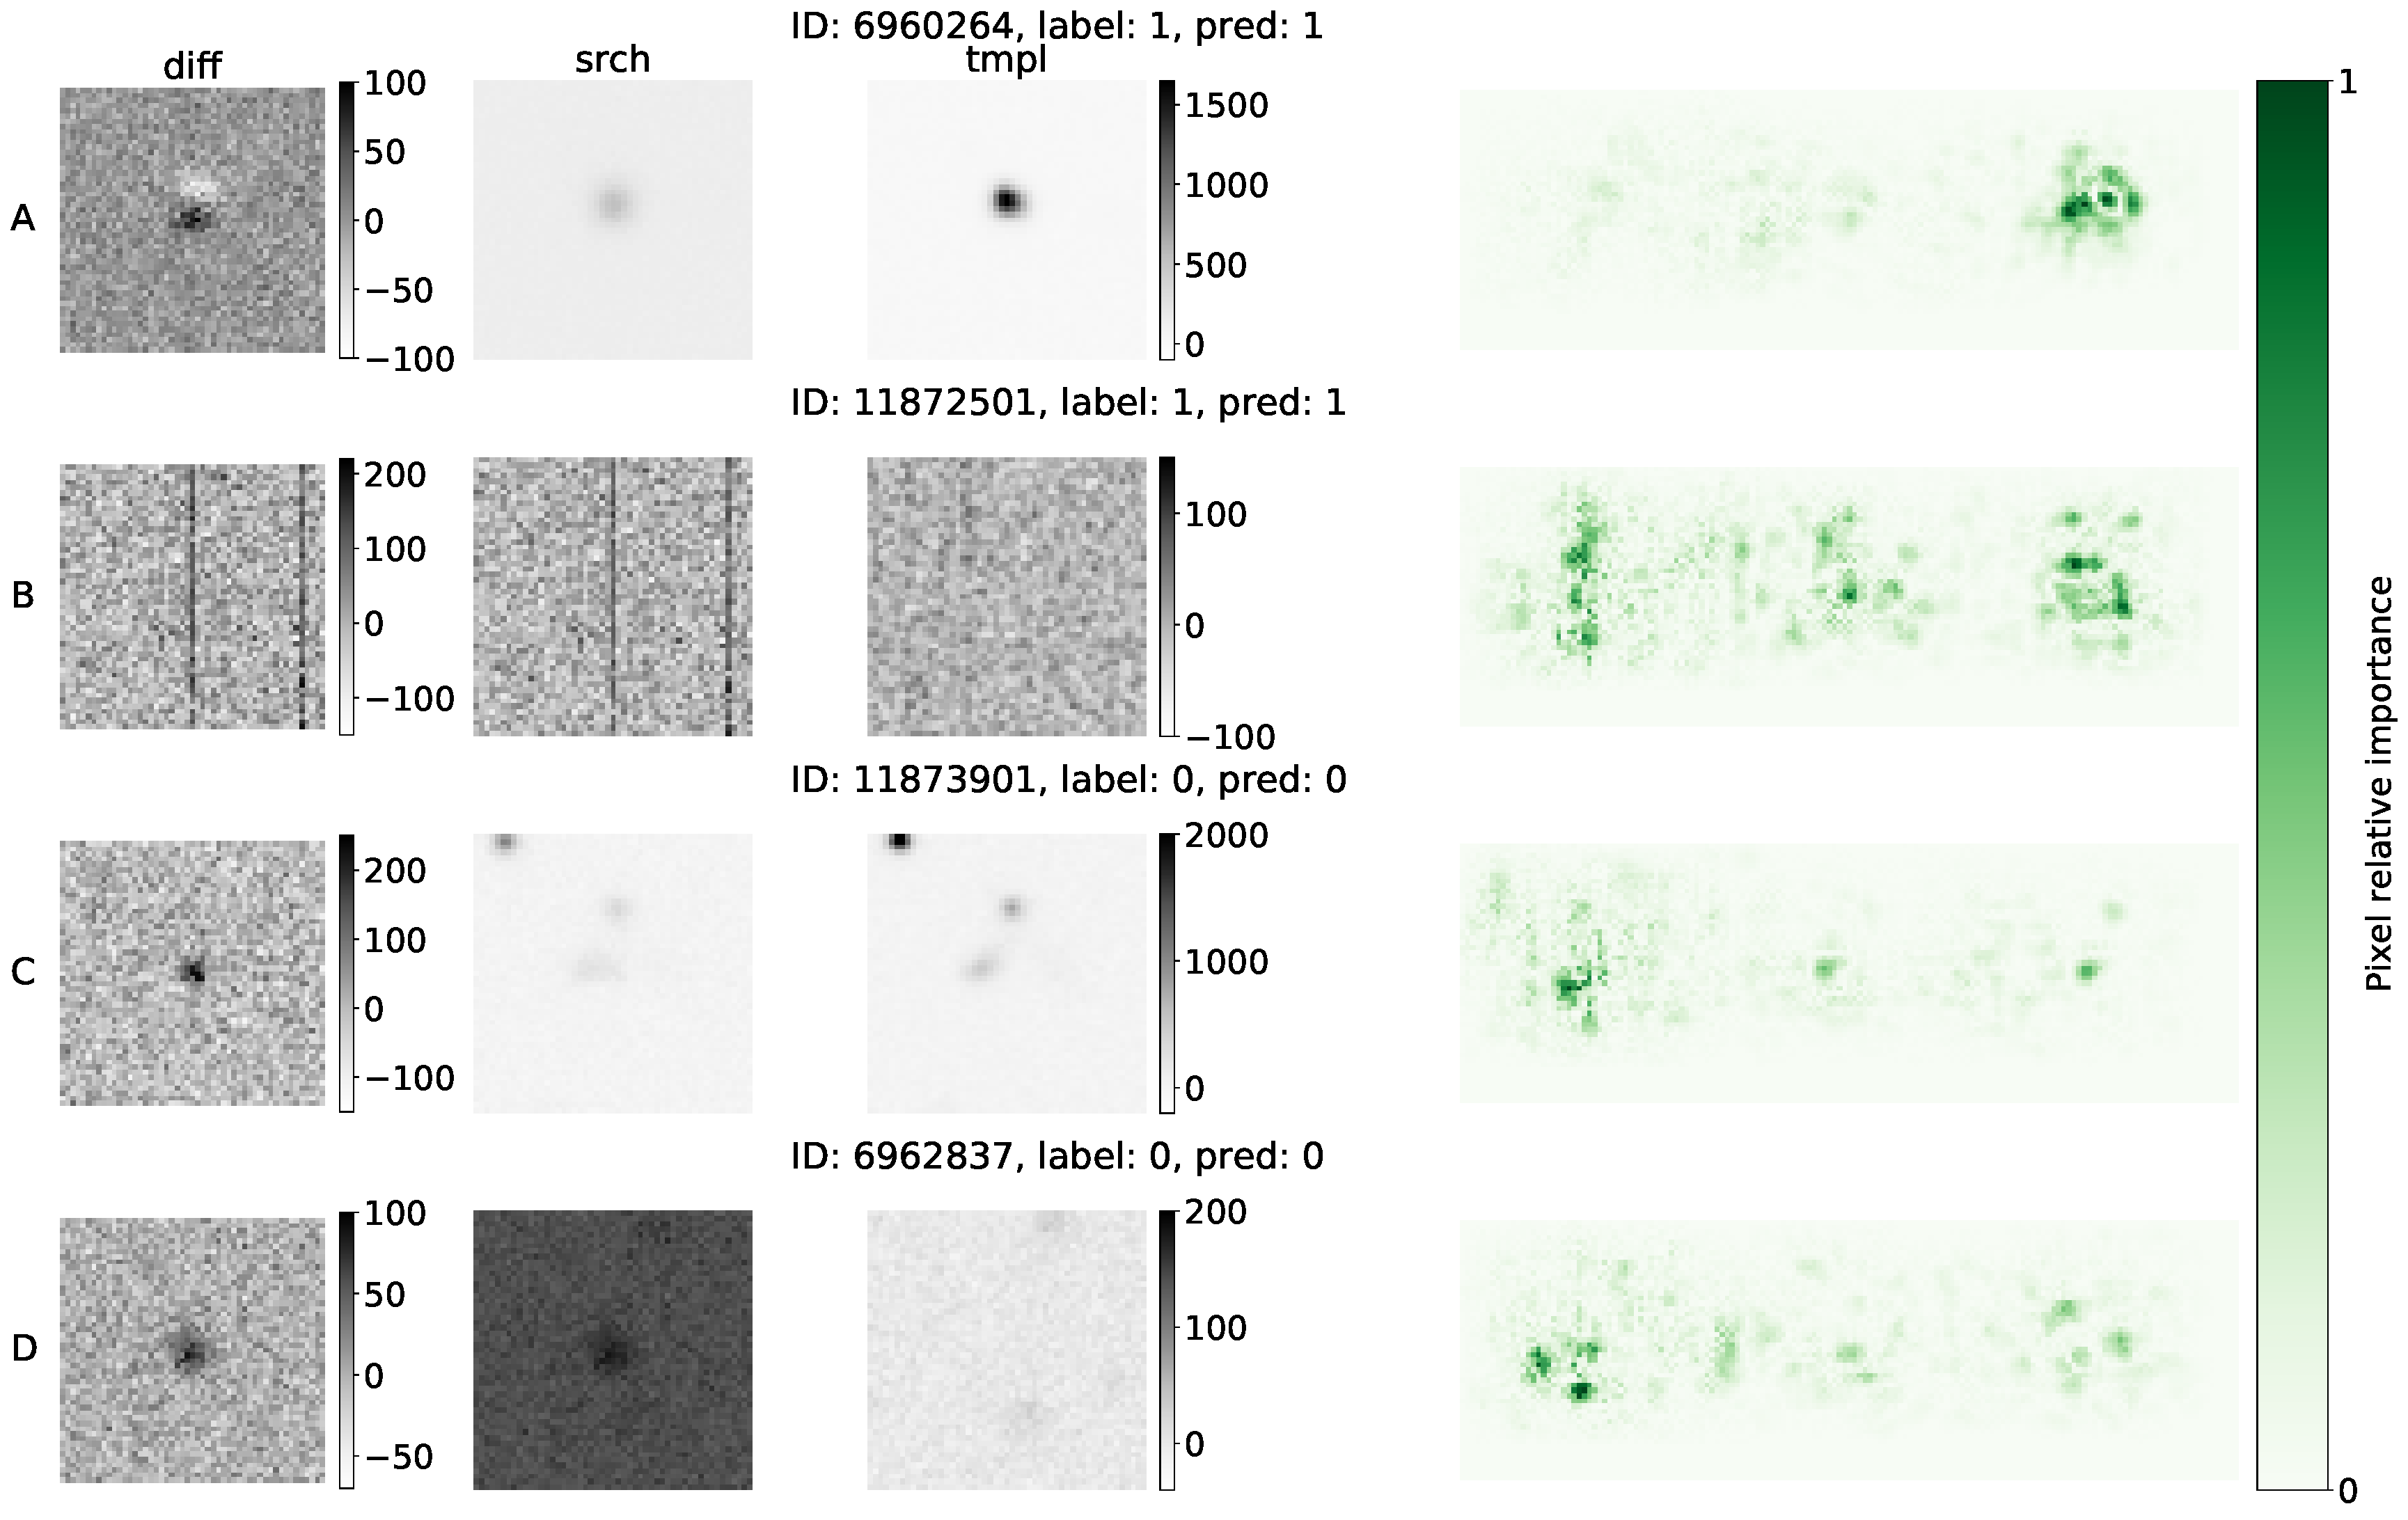
\includegraphics[width=0.9\linewidth]{
    figures/saliency_plot.pdf}
    \caption{Saliency map for the four transients in \autoref{fig:examples_no_normalization} for the \diabased\ model. On the left, in grey color, the original \diff, \search, and \temp\ images are plotted in their natural flux scale (before normalization). On the right, the saliency map for the combined image. The intensity of a pixel color in the white-to-green scale indicates the pixel relative importance: the maps are normalized to 1 individually, such that dark green corresponds to high saliency score, with 1 corresponding to the most important pixel in the image triplet. With the side-by-side organization of the input data, these maps enable a visual understanding of the importance of each element of the combined image in the real-bogus classification. We note how in some cases (panel A) the decision is largely based on the \temp, rather than the \diff\ image, and in some cases all three image elements contribute similarly to the decision (panel B). This figure is discussed in more detail in \autoref{subsec: saliency}.}
    \label{fig:saliency_4id}
\end{figure*}

\begin{figure*}
    \centering
    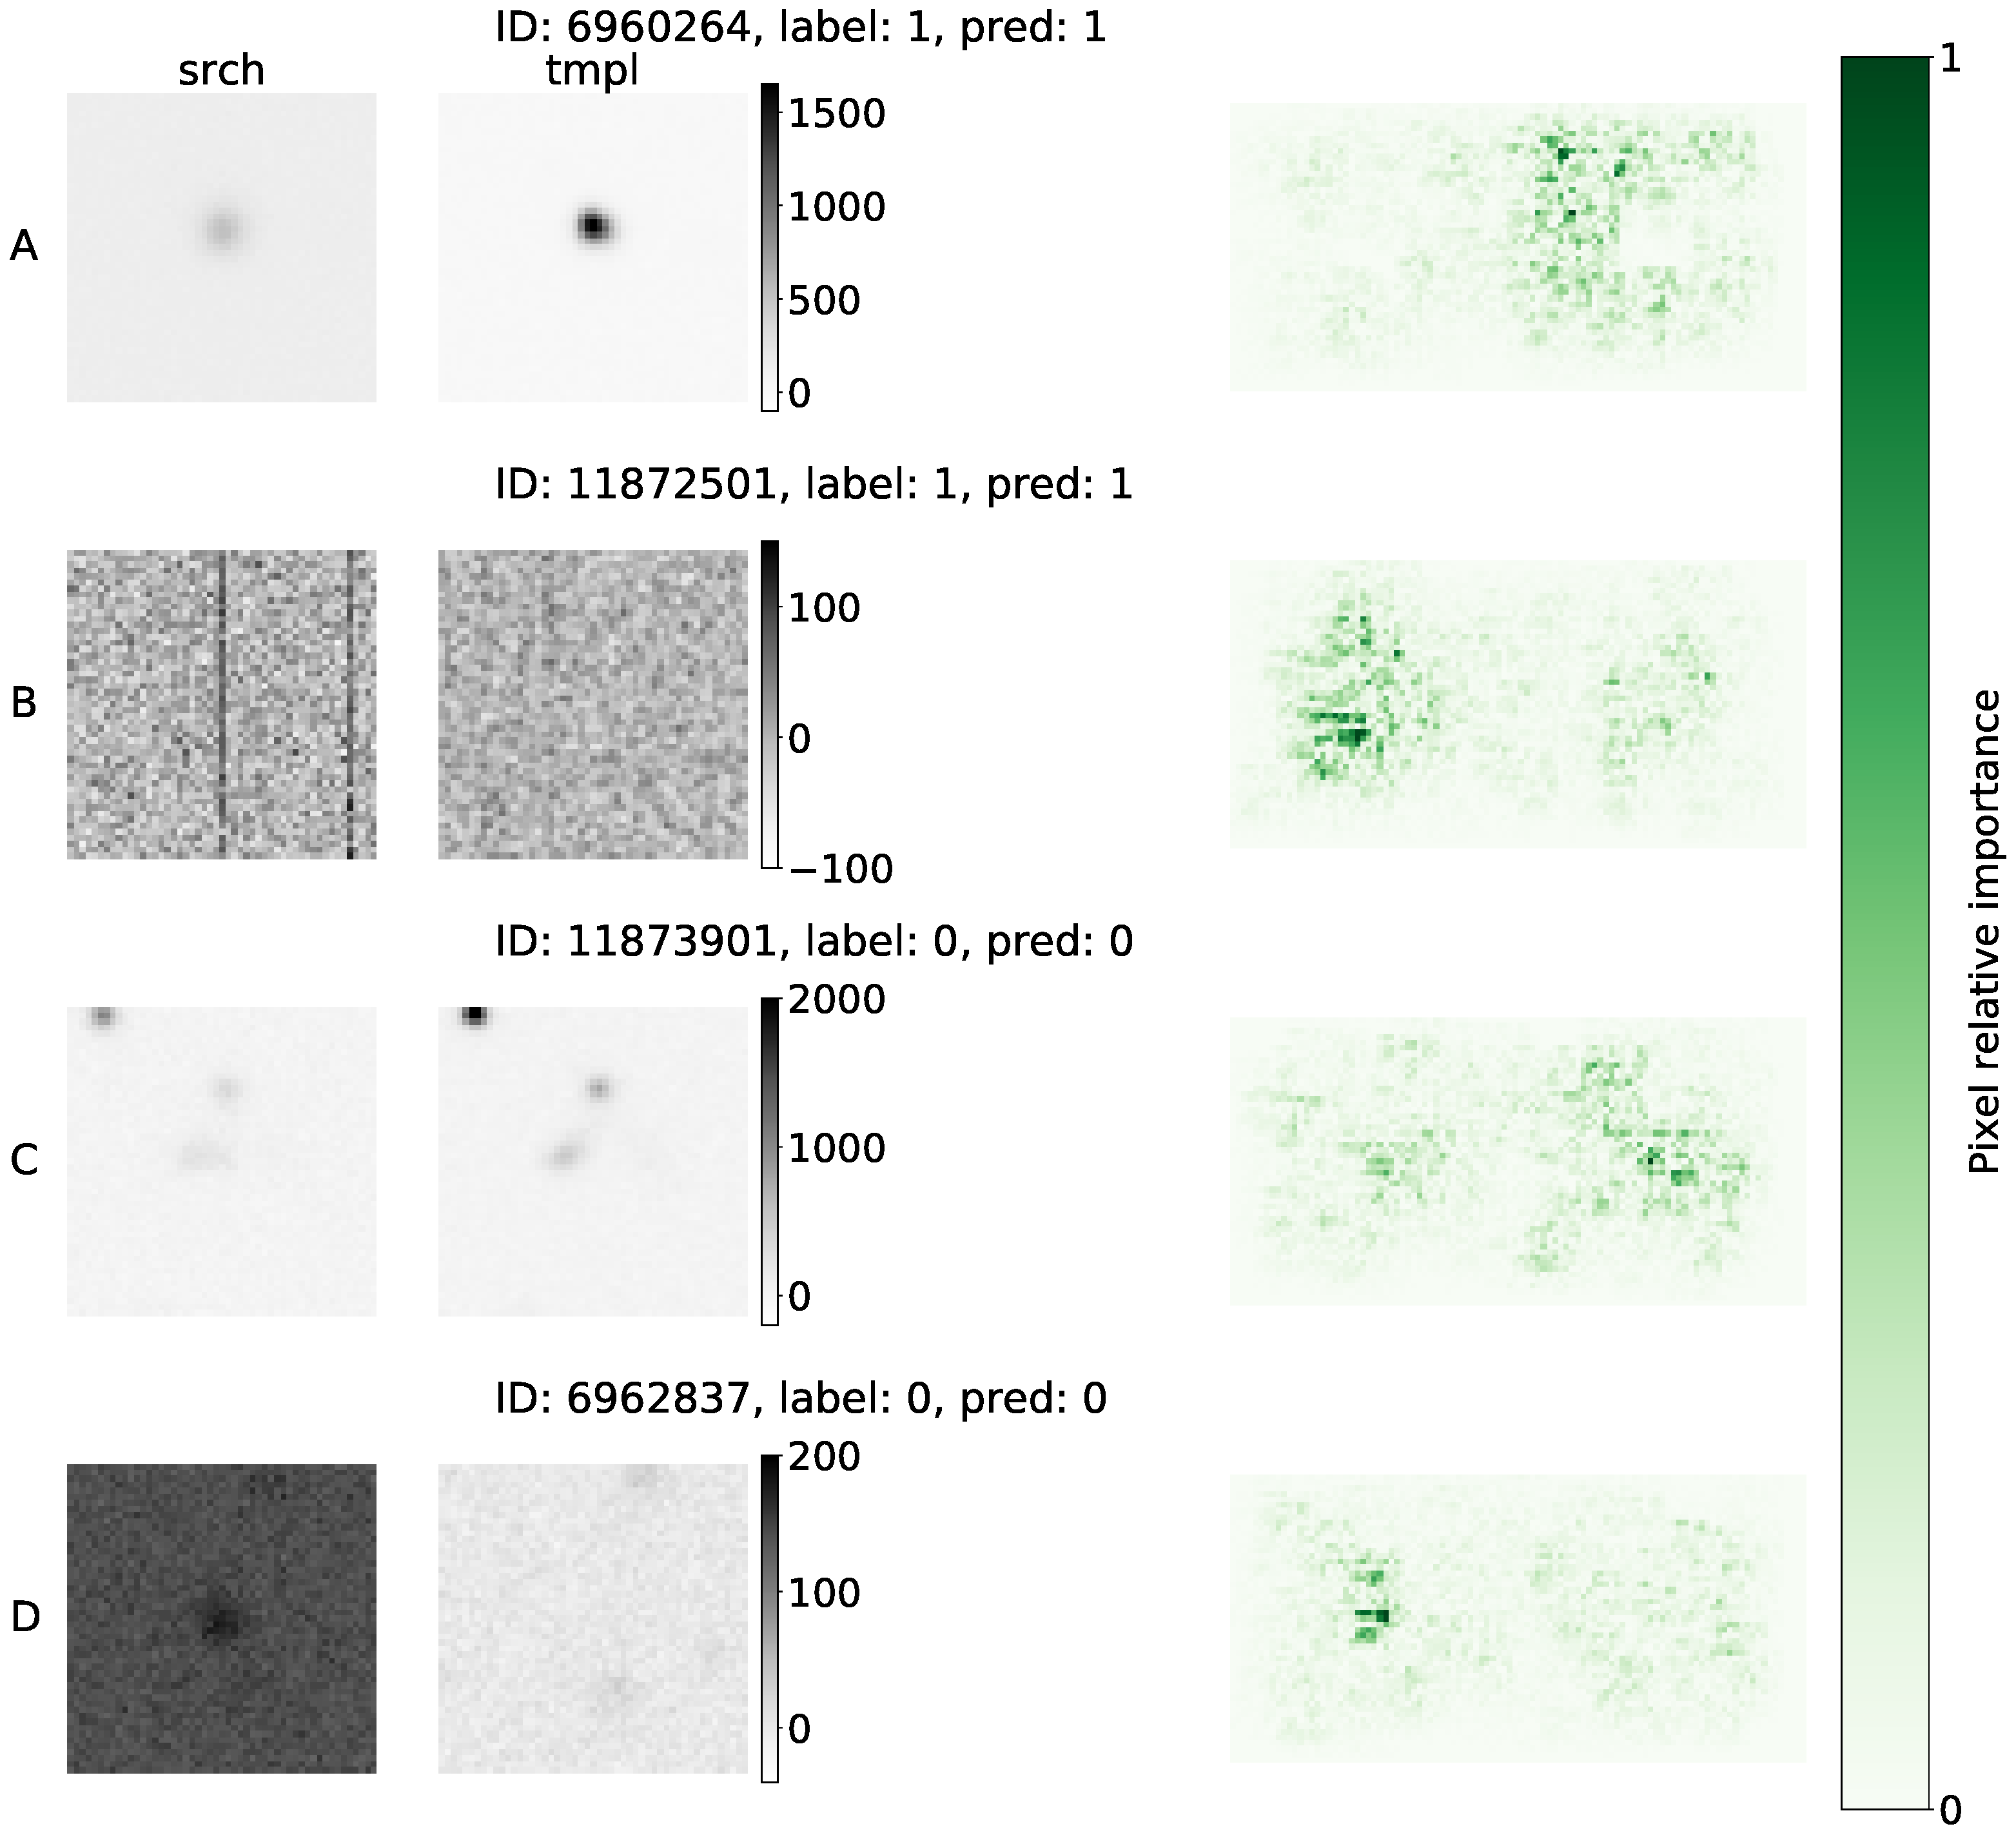
\includegraphics[width=0.84\linewidth]{
    figures/saliency_plot_noDIA.pdf}
    \caption{As \autoref{fig:saliency_4id} but for the \nodia\ model: saliency map for the four transients in \autoref{fig:examples_no_normalization}. This figure is discussed in more detail in \autoref{subsec: saliency}.}. 
    \label{fig:saliency_4id_noDIA}
\end{figure*}


% \begin{figure*}
% \begin{minipage}[b]{0.45\linewidth}
%     \centering
%     \includegraphics[width=1\linewidth]{
%     figures/ROC3D.pdf}
%     \caption{ROC curve for the $20,000$ images used for testing the \textbf{\diabased\ }model. The area under the curve was $0.992$.}
%     \label{fig:roc_modelAAA}
% % \end{figure}
% \end{minipage}
% \begin{minipage}[b]{0.45\linewidth}
% % \begin{figure}[H]
%     \centering
%     \includegraphics[width=1\linewidth]{
%     figures/ROC.pdf}
%     \caption{ROC curve for the $20,000$ images used for testing the \textbf{\nodia\ }model. The area under the curve was $0.973$.}
%     \label{fig:roc_modelCCC}
%     \end{minipage}
% \end{figure*}
\subsection{A peek into the model decisions through saliency maps}\label{subsec:results_seliancy}


% \masao{This is a very interesting section!  For readers like me who don't know much about how saliency maps are produced, can you write a couple of sentences about how they are made?  I think you said something about removing each pixel and looking at how much the predictions change.  A short description is helpful for the uneducated reader like me.}



\begin{figure*}
        \centering
    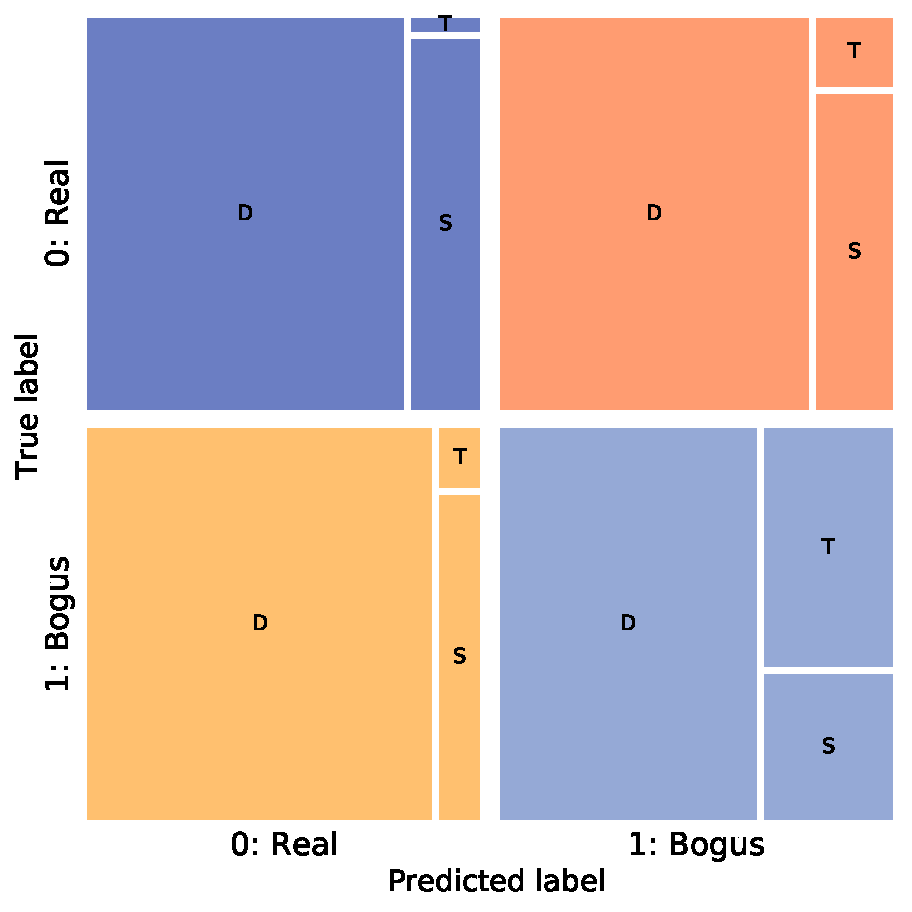
\includegraphics[width=0.45\linewidth]{
    figures/confusionmatrix_NERSCsaliencyDIA_100K20KNERSCstam0-9CCCC_3s3DH.pdf}
     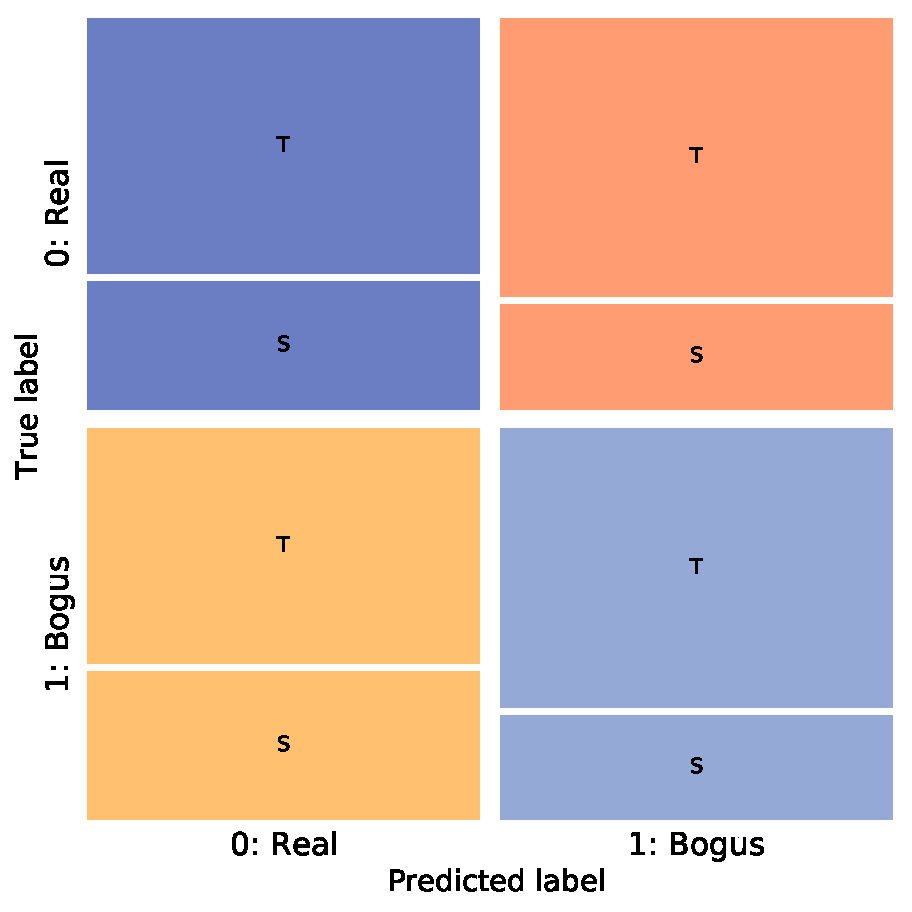
\includegraphics[width=0.45\linewidth]{
    figures/confusionmatrix_NERSCsaliencynoDIA_100K20KNERSCstam0-9CCCC_3s2DH.pdf}
    \caption{Confusion matrix reporting the proportion of transients for which the highest concentration of important pixels is found in the \diff, \search, or \temp\ portion of the input image for the \diabased\ model results (left) and \nodia\ model (right), {\it Left}: \diabased. For 80\% ($7683$) of the $9571$ transients classified correctly as ``real'', the classification principally relied on the the \diff\ image ($I_\diff > 1/3$); for 18\% ($1758$) on the the \search ;  and for 1\% ($130$) on the the \temp . For incorrect ``real'' classifications 88\% of the images relied principally on \diff\,10\% on \search, and 2\% on \temp. For incorrect ``bogus'' classifications 79\% of the images relied principally on \diff\, 17\% on \search, and 4\% on \temp. For correct ``bogus'' classifications 66\% of the images relied principally on \diff\, 13\% on \search, and 21\% on \temp. {\it Right}: \nodia. Of the $9163$ transients classified correctly as ``real'', for 66\% of them, the classification relied principally on the \temp\ image. For the incorrect ``real'' classifications 61\% of the cases were principally based on the \temp. For the incorrect ``bogus'' classifications 71\% of the cases were principally based on the \temp. For correct ``bogus'' classifications 72\% of the cases were principally based on the \temp. }
    \label{fig:saliency_confusions}
\end{figure*}

%A gradient of the final output with respect to the input data is the operation used to calculate the score. 
%A saliency map provides a score to each one of the pixels that form the image used for training the CNN base on how important is that pixel to the final classification of the CNNs. A gradient of the final output with respect to the input data is the operation used to calculate the score. 
%For the purpose of this work the score range is not relevant, we focus only on the value given by the code and that a higher value implies a more relevant pixel for the classification. A higher score of a pixel would indicated that a small change in that flux value would affect the final output, and consequently the final classification decision. 
%Our expectation is that pixels scored highly are located in the object that we want to classify. 

\begin{figure*}
    \centering
    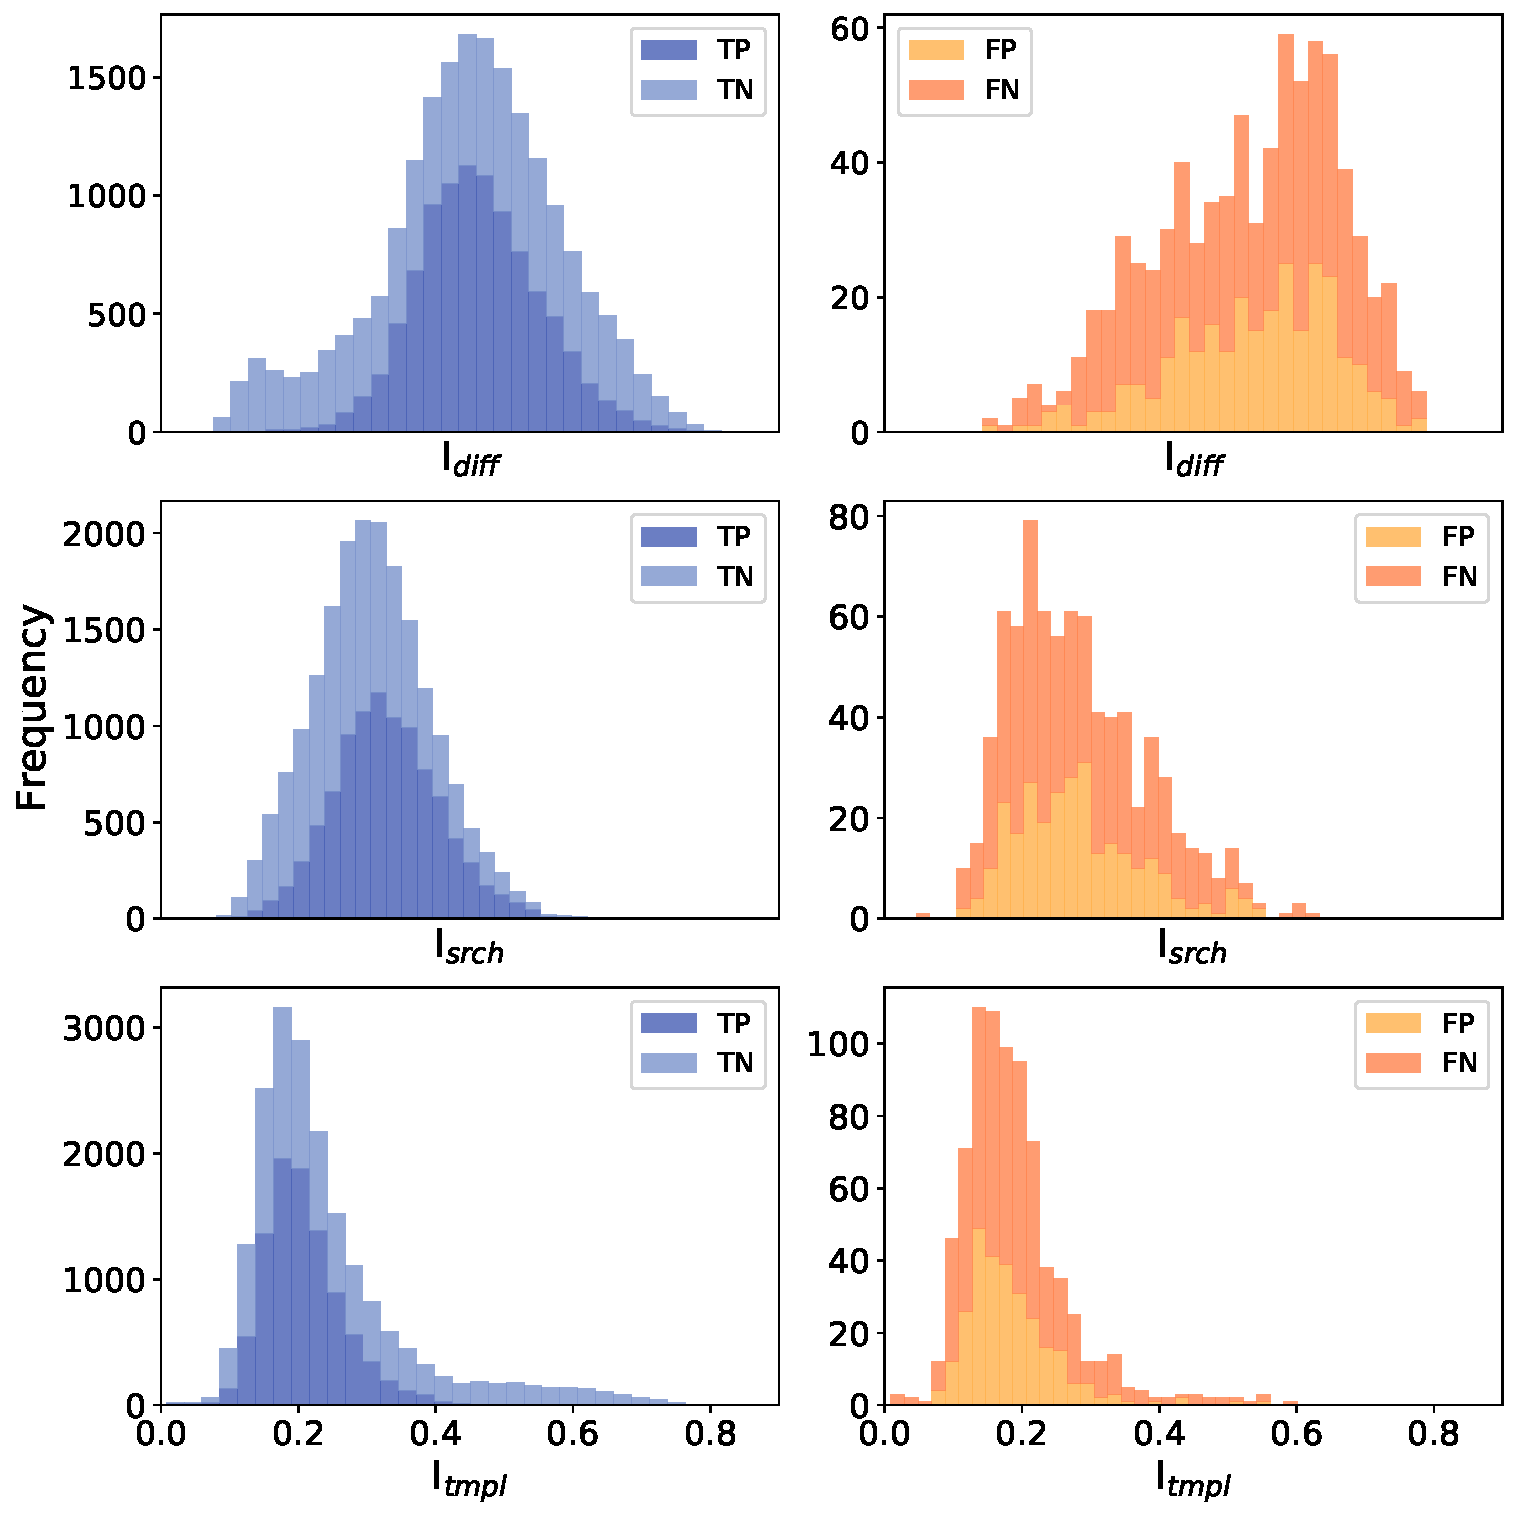
\includegraphics[width=0.45\linewidth]{
    figures/histogram_sm_important_pixels_NERSC100K20KNERSCstam0-9CCCC_3s3DH.pdf}
    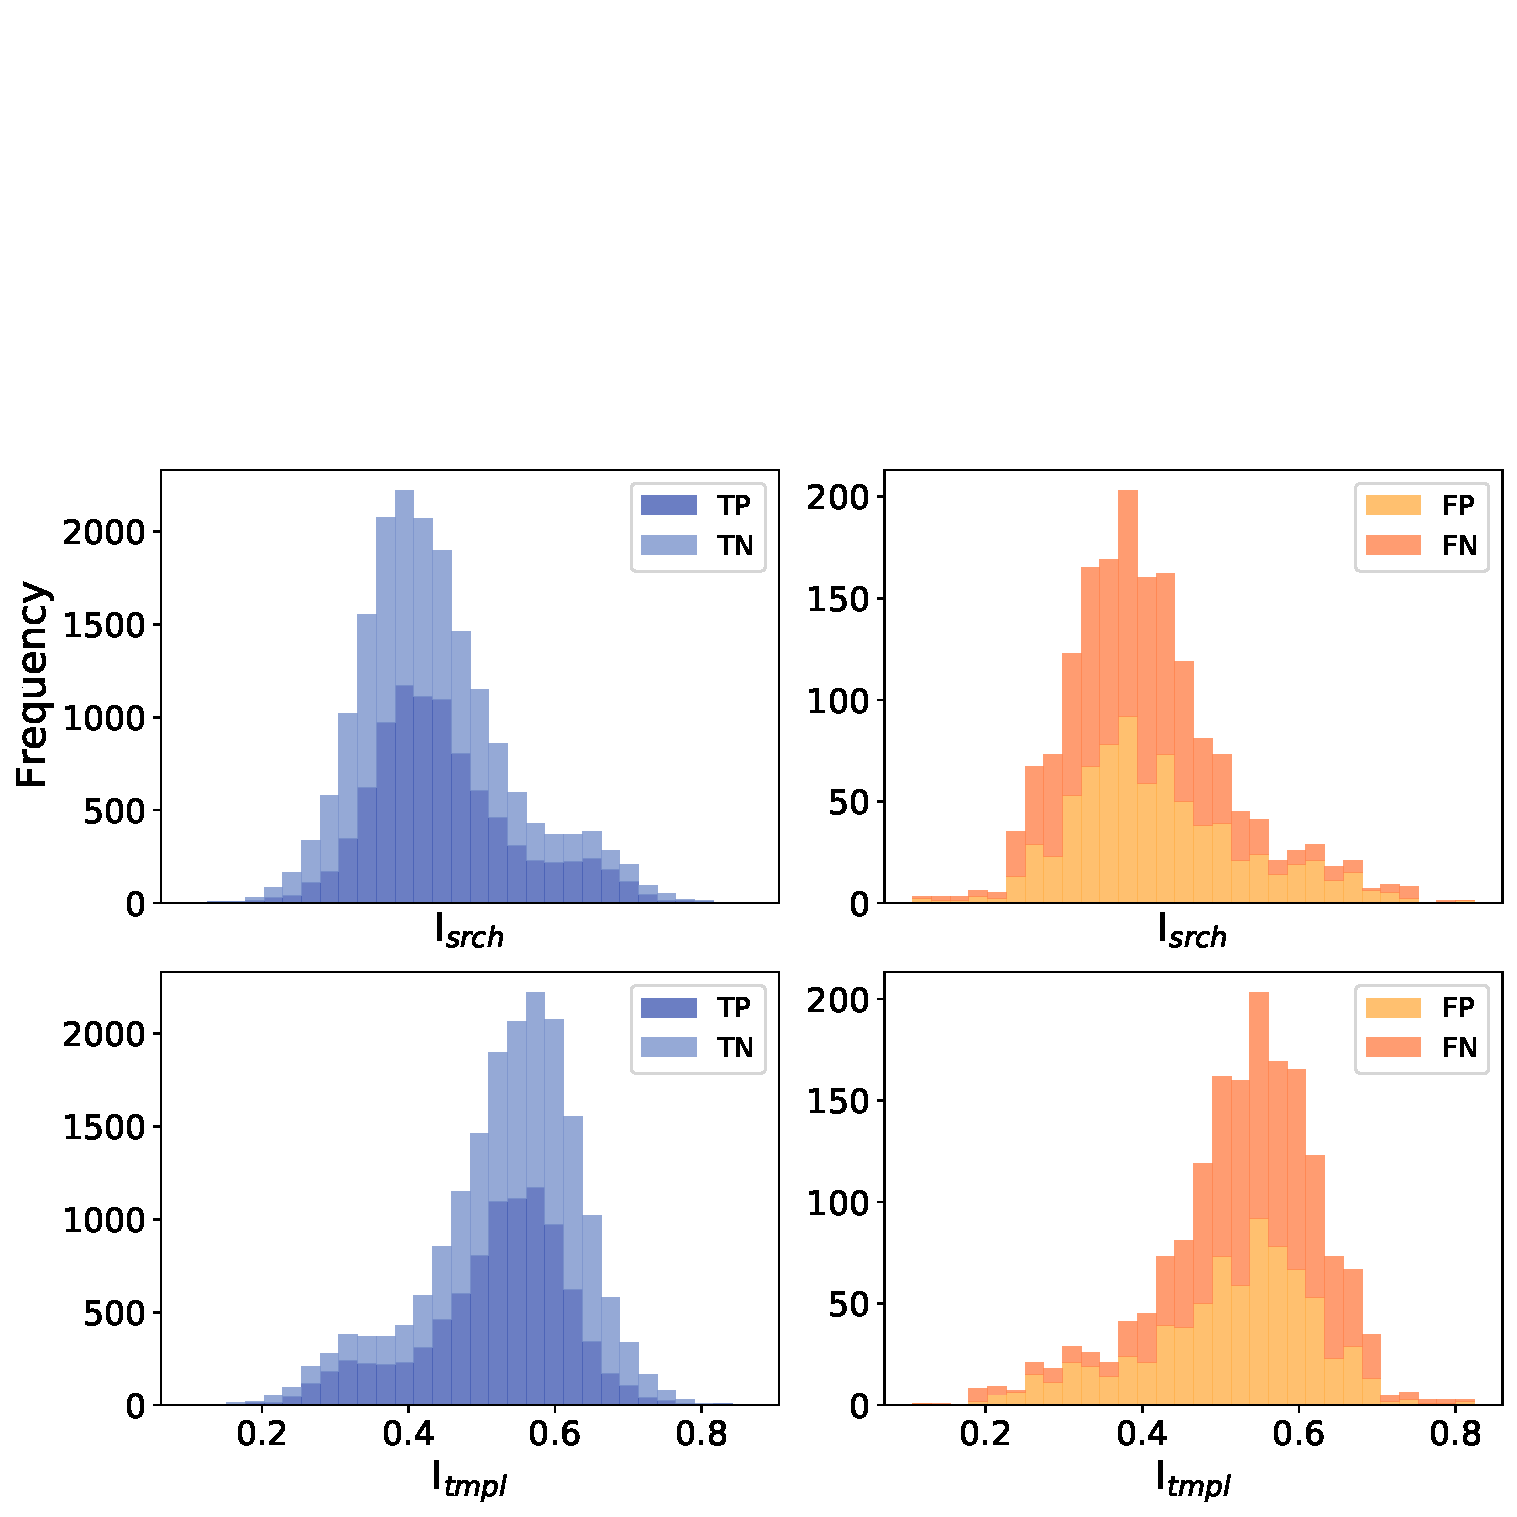
\includegraphics[width=0.45\linewidth]{
    figures/histogram_sm_important_pixels_NERSC100K20KNERSCstam0-9CCCC_3s2DH.pdf}
    \caption{The distribution of  $\idiff$ (top), \isearch\ (middle), and \itempl\ (bottom) value for the 20,000 transients in the test data (see \autoref{eq: saliencymetric}). The colors corresponds to the quadrants of the confusion matrix to which the transient belong according to the model prediction, \diabased\ predictions in the first and second column from the left to the right and \nodia\ in the third and fourth. Blue shades correspond to correct predictions (TP and TN) and orange to FP and FN. Note that the $y$ axis values are different in each plot and the FP and FN histograms contain far fewer observations. On the {\itempl\ Left}, for the \diabased\ model, the TP classification shows a preference for the \diff\ images and the distribution peaks at $\idiff \sim 0.5$. For TN, however, small $\idiff$ values are more common, with an significant fraction of observations in the $0<$\idiff$<0.33$ region. This behaviour is complemented by a long \itempl\ tail in the TN distribution ($0.4<\itempl<0.8$). The FP and FN distributions are qualatively similar to the TP and TN, but noisier, as they contain fewer than 10\% of the objects. {\it Right}: \nodia\ model. All four classes have qualitative similar distributions in \itempl and \isearch. Classifications rely mostly on the \temp\ in all cases ($\itempl > 0.5$)}
    \label{fig:histo_saliency}
\end{figure*}


In \autoref{subsec:scaling}, we described how the importance of individual image pixels in the RB prediction performed by our models can be measured, and the design of a saliency-based metric to assess which component of the image is most important to perform the RB classification. Here we inspect the saliency maps, both visually and quantitatively through the measured values of \idiff, \isearch, and \itempl. 


In \autoref{fig:saliency_4id} and \autoref{fig:saliency_4id_noDIA} we show the four transients we considered as examples throughout this work, the same images used in \autoref{fig:examples_no_normalization} and \autoref{fig:examples_hstack_normalization}, and the corresponding saliency maps for the \diabased\ model and \nodia\ model respectively. \autoref{fig:saliency_confusions} and \autoref{fig:histo_saliency} report the results of \autoref{eq: saliencymetric} for the objects in our training set.

Lets start with some considerations about the saliency maps for the four image examples for the \diabased\ model (\autoref{fig:saliency_4id}), and specifically from  panels C and D were the transients were correctly predicted as ``real''. We observe that the greatest concentration of important pixels for both these images is found in the left-most third of the image: %the \diff\ section, \question{approx the 50\% of all the pixels that form the triple in the saliency map}, meaning that
$\idiff \sim 0.5 $ for both. 
%, according to the definition in \autoref{eq: saliencymetric}.
We speculate, from our experience in labeling real/bogus by visual inspection and consulting with some of the human scanners that labeled the original \texttt{autoscan} images, that this behaviour is similar to what a human scanner would do: if in the \diff\ image there is a clearly real transient, the scanner would not need to study in detail the \search\ and \temp\ images. 

\autoref{fig:saliency_4id}A and B show correctly classified ``bogus'' transients. In \autoref{fig:saliency_4id}A, a ``bogus'' produced likely by a moving object displaying a classical dipole, the majority of the important pixels are located in the \temp\ ($\itempl \sim 0.54 $), concentrated around the location of the central source and the location  where its ``ghost'' image is (the coordinates corresponding to the location the bright patch of pixels in the \diff, but in the \temp\ portion of the composite image).
In \autoref{fig:saliency_4id}B, there is no central source and the detection is triggered by an image artifact. The important pixels are found in all three image segments and are spread around a large area of each image: the model has inspected the image in its entirety to decide the classification. 
Following our consideration about the similarity between the CNN and human decision process, we speculate that here too the CNN  mimics closely what a human scanner would do: because there is not a clear central source (a ``real'' object) in the \diff, the scanner would analyze the \search\ and \temp\ images to extract more information from the context to enable a classification. However, it should be noted that no quantitative studies of the features the human scanners use to classify transients has been done, thus this remains simply an intriguing suggestion.



For the case of the \nodia\ model, the expectation was less clear: both the \search\ and the \temp\ images are necessary to ``reconstruct'' the information contained in the \diff, and while the pixels overlapping with the central transient are obviously expected to be important, the pixels that surround it are necessary to essentially reproduce the scaling and PSF-matching operations between \temp\ and \search\ that the DIA performs. 
Accordingly, the saliency maps presented in \autoref{fig:saliency_4id_noDIA} are more difficult to interpret: in all four cases, important pixels are found all over the composite images.
%the results, that are presented graphically in right \autoref{fig:histo_saliency} and right \autoref{fig:saliency_confusions}, are more difficult to interpret.

To explore how the choice of important pixels may depend on the image label and on the correct classification we report  the fraction of images for which the \diff\ (\search, \temp) is the dominant source of important pixels {\it within} the confusion matrix in \autoref{fig:saliency_confusions}. To do this, we use a rough but intuitive cutoff: if the normalized sum of the saliency pixels in a third of the image is larger than $\frac{1}{3}$, then we deduce that the model principally used that component for its decision. For example, where $\idiff > 0.33$, we conclude that the model principally relied on \diff\ to make the RB classification. With this cut-off we can assess if there are differences in the model behavior when classifying objects as a function of their labels or their classification.
In all four cases (all combinations of ``real'' and ``bogus'' label and prediction) the concentration of important pixels is largest in the portion of the image corresponding to the \diff\  in the \diabased\ model. It is however interesting to note that, in order to correctly classify the ``bogus'', the \diabased\ model uses the template and search image more heavily than in all other cases (\diff, \search, \temp,  = 66\%, 13\%, 21\% for TN, while $I_\diff>80\%$ for TP, FP, and FN). 

The cut-off method described above does not allow us to distinguish between cases where multiple sections of the images were used jointly, perhaps with similar importance, from cases where the model truly only relied on one section of the image. For that, we take a closer look at the distribution of saliency values. 
In \autoref{fig:histo_saliency} we show the distribution of values of the three metrics defined in \autoref{eq: saliencymetric} for each of the four cases: TP and TN, in shades of blue, FP and FN, in shades of orange, following the color-scheme adopted in \autoref{fig:confusiomatrix_models} and \autoref{fig:saliency_confusions}. For the \diabased\ model (the two left-most columns), for the majority of the 20,000 images in the training set $\idiff > 0.33$, but there is a secondary pick in the $\idiff$ distribution near $\idiff \sim0.1$ populated entirely by TN cases, complementary to a long right tail in the \itempl distribution ($\itempl > 0.4$). This confirms that the correct classification in the presence of real transients relies on \diff, but \temp\ and \search\ become important to correctly classify bogus transients, just like we had seen in the exemplary cases in \autoref{fig:saliency_4id}. We note also that the general shape of each distribution (\idiff, \isearch, \itempl) is similar for the TP and TN case (blue) and for the FP and FN cases (orange). 
 
For the \nodia\ model the important pixels are concentrated in the \temp\  for most images ($\itempl > 0.5$) for both correct and incorrect classifications.
This is somewhat counter-intuitive since the \temp\ {\it does not} contain the transient itself! However, one may speculate that this is because the \temp, a higer quality image, contains more accurate information about the context in which the transient arises: \eg, if it is located near a galaxy or not. This information is important to the classification. It is also interesting to note that for the transients predicted as ``real'' in both TP and FP, the fraction of images that leveraged primarily the \temp\ is approximately $2/3$, and for images predicted as ``bogus'', in both TN and FN, it is approximately $3/4$.

To help guide the interpretation of the saliency maps, a few more maps are plotted in \hyperref[sec:appendixc]{Appendix D}. Where we provide 6 examples per each class of the confusion matrix, for both the \diabased\ and the \nodia\ models. 

\subsection{Computational cost of our models}\label{sec:computationcost}
The computational cost of our models, reported in CPU Node hours in \autoref{tab:acc results}, confirms that while training a CNN model for RB can be computationally expensive, and significantly more so if the \diff\ is not used in input (\nodia), the model prediction is instantaneous. Using a NN-based platform, the computational costs are front-loaded. In transient detection this could mean that the observation-to-transient discovery process is instantaneous, while computation time can be spent during off-sky hours (principally to build templates). Furthermore, while the training time is longer for the \nodia\ model than for the model that uses the \diff\ in input (\diabased) the computational cost of the forward-pass (prediction) scales superlinearly with the size of the feature set (pixels), so that our \nodia\ model takes less than half the time than the \diabased\ one to perform the RB task. With a clock time of 0.3 ms per 51$\times$51 pixels postage stamp, predicting over the full DES focal plane would take $\sim 1$ minute. However, we note that at this stage of our work we still rely on the DIA in several ways: while the \temp\ and \search\ in input to \nodia\ are not PSF matched, this proof of concept is performed on transients that were detected in \diff\ images, and we leverage the alignment of \temp\ and \search\ and centering of the postage stamp that arose from the DIA (see \autoref{sec:futurework}). Conversely, predictions would only need to be done in correspondence of the sources detected in the \temp\ and \search\ images, and not for the entire CCD plane.




% \begin{figure*}
% \begin{minipage}[b]{0.45\linewidth}
%     \centering
%     \includegraphics[width=0.8\linewidth]{
%     figures/confusionmatrix_saliencyDIA(1).pdf}
%     \caption{Confusion matrix and the proportion of the most important pixels given by the saliency map of each of the images in the triple after the training using the \textbf{\diabased\ }model. i.e., from the $9564$ transients classified correctly as ``real'', 90\% ($8630$) of them, the classification was done based principally on the \diff\ image due to the fact that the sum of pixels in the \diff\ section in the saliency map was the greatest of the three. }
%     \label{fig:saliency_confusionDIA}
% \end{minipage}
% \begin{minipage}[b]{0.45\linewidth}
%     \centering
%     \includegraphics[width=0.8\linewidth]{
%     figures/confusionmatrix__saliencynoDIA.pdf}
%     \caption{Confusion matrix and the proportion of the most important pixels given by the saliency map of each of the images in the duplex after the training using the \textbf{\nodia\ }model. i.e., from the $9147$ transients classified correctly as ``bogus'', 24\% ($2197$) of them, the classification was done based principally on the \search\ image due to the fact that the sum of pixels in the \search\ section in the saliency map was the greatest of the two. }
%     \label{fig:saliency_confusionnoDIA}
%     \end{minipage}
% \end{figure*}






\section{Future work and limitation of this work}\label{sec:futurework}
This work is targeted to the investigation of CNN RB model performance, with and without \diff\ in input, on a single data set, the same dataset upon which the  development of the random-forest-based \texttt{autoscan} was based (see \autoref{sec:data}). This approach enables a straightforward comparison, but it comports some limitations. 

The labels in our data set come from simulations of SNe ($\texttt{label = 0}$) and visual inspection that classifies artifacts and moving objects ($\texttt{label = 1}$). We reserve to future work the investigation of the efficacy of the model on transients of different nature, including quasars (QSOs), strong lensed systems, Tidal Disruption Events (TDEs), and supernovae of different types.  These transients may have characteristically different associations with the host galaxy, including preferences for different galaxy types and locations with respect to the galaxy center, compared to the simulated SNe events in our training set. 

Specifically thinking of Rubin LSST data, an additional source of variability may be introduced by Differential Chromatic Refraction effects \citep{Abbott_2018, richards2018leveraging}, or stars with significant proper motion which, due to exquisite image quality of the Rubin images, would be detectable effects.

While we demonstrated CNN model's potential in the detection of transients without DIA, we did not address the question of completeness as a function of \search\ or \temp\ depth or the potential for performing accurate photometry without DIA. 

Improvements in the \nodia\ model performance could be achieved by considering %rotation invariance, 
alternative network architectures, more training epochs, tuned hyperparameters, {\it etc}., and we leave these tasks as future work beyond the proof-of-concept presented here. %The optimization of the architecture would be included for a future work. 

Finally, we note that our models did in fact implicitly leverage some of the information generated by the DIA even when they did not use the \diff\ image itself as input.  First, the \temp\ and \search\ images are de-warped. Since the transient alerts are generated from aligned DIA images, the transient source is always located at the image center in our data. We use postage stamps that were, however, not PSF matched or scaled to match the template brightness.
To move beyond a proof-of-concept, in future work we will re-train and apply our models to images whose alignment does not depend on the existence of a transient. %This would support strongly that the used of the \diff\ image is not necessary because nowadays the position of the source in the image-triplet is done based in the \diff\ image.
%\clearpage
\section{Conclusions}\label{sec:conclusion}


In this work, we have demonstrated that high-accuracy models for classifying true astrophysical transients from artifacts and moving objects (a task generally known as ``real-bogus'') can be built without leveraging the results of a difference image analysis (DIA) pipeline that constructs a ``template-subtracted'' image.

Starting from the Dark Energy Survey dataset that supported the creation of the well known real-bogus \texttt{autoscan} model \citep{Goldstein_2015}, we first built a CNN-based model, dubbed \diabased, that uses a sky template (\temp), a nightly image (\search), and a template-subtracted version of the nightly image (\diff) that performs real-bogus classification at the level of state-of-the art models.  Our \diabased\ model reaches a state-of-the art $97\%$ accuracy in the bogus classification with an Area-Under-the-Curve of 0.992 and does not require human decision in the feature engineering or extraction phase.

We then created \nodia, a model which uses only the \temp\ and \search\ images and can extract information that enables the identification of bogus transients with $92\%$ accuracy even with a naive model architecture that, to enable a direct comparison, is purposefully designed to be minimally different from our high accuracy \diabased\ model.

We further investigated what information enables the real-bogus classification in both the \diabased\ and \nodia\ models and demonstrated that a CNN trained with the DIA output primarily uses the information in the \diff\ image to make the final classification, and that the model examines a \diff-\search-\temp\ image-set fundamentally differently in the cases where there is a transient, than in the cases where there is not one. The \nodia\ model, conversely, takes a more comprehensive look at both \temp\ and \search\ images, but relies primarily on \temp\ to enable the reconstruction of the information found in the \diff.

Implementation of this methodology in future surveys could reduce the time and computational cost required for classifying transients by entirely omitting the construction of the difference images.  

\clearpage
\section{Acknowledgment}\label{sec:thanks}
 
 
TAC and FBB acknowledge the support of the LSST Corporation and the Enabling Science Grant program that partially supported TAC through Grant No. 2021-040, Universidad Nacional de Colombia and University of Delaware for the Beyond Research Program (2020) and Summer Research Exchange (2021). MS and HQ were supported by DOE grant DE-FOA-0002424 and NSF grant AST-2108094. 

TAC: Prepared the data, conducted the analysis, created and maintains the machine learning models, wrote the manuscript.
FBB: Advised on data selection,  curation, and preparation,  selection and design, revised the manuscript.
GD: Advised on data preparation and model selection and design, revised the manuscript.
MS: Advised on data selection, shared knowledge about the compilation and curation of the original dataset, revised the manuscript.
HQ: Advised on data preparation and model design, revised the manuscript.


 This paper has undergone internal review in the LSST Dark Energy Science Collaboration.
 The internal reviewers were: Viviana Acquaviva, Suhail Dhawan, and Michael Wood-Vasey.
 
 
 
% This work used some telescope which is operated/funded by some agency or consortium or foundation ...
% We acknowledge the use of An-External-Tool-like-NED-or-ADS.
The DESC acknowledges ongoing support from the Institut National de 
Physique Nucl\'eaire et de Physique des Particules in France; the 
Science \& Technology Facilities Council in the United Kingdom; and the
Department of Energy, the National Science Foundation, and the LSST 
Corporation in the United States.  DESC uses resources of the IN2P3 
Computing Center (CC-IN2P3--Lyon/Villeurbanne - France) funded by the 
Centre National de la Recherche Scientifique; the National Energy 
Research Scientific Computing Center, a DOE Office of Science User 
Facility supported by the Office of Science of the U.S.\ Department of
Energy under Contract No.\ DE-AC02-05CH11231; STFC DiRAC HPC Facilities, 
funded by UK BIS National E-infrastructure capital grants; and the UK 
particle physics grid, supported by the GridPP Collaboration.  This 
work was performed in part under DOE Contract DE-AC02-76SF00515.

 This project used public archival data from the Dark Energy Survey (DES). Funding for the DES Projects has been provided by the U.S. Department of Energy, the U.S. National Science Foundation, the Ministry of Science and Education of Spain, the Science and Technology Facilities Council of the United Kingdom, the Higher Education Funding Council for England, the National Center for Supercomputing Applications at the University of Illinois at Urbana–Champaign, the Kavli Institute of Cosmological Physics at the University of Chicago, the Center for Cosmology and Astro-Particle Physics at the Ohio State University, the Mitchell Institute for Fundamental Physics and Astronomy at Texas A\&M University, Financiadora de Estudos e Projetos, Fundação Carlos Chagas Filho de Amparo à Pesquisa do Estado do Rio de Janeiro, Conselho Nacional de Desenvolvimento Científico e Tecnológico and the Ministério da Ciência, Tecnologia e Inovação, the Deutsche Forschungsgemeinschaft and the Collaborating Institutions in the Dark Energy Survey. The Collaborating Institutions are Argonne National Laboratory, the University of California at Santa Cruz, the University of Cambridge, Centro de Investigaciones Enérgeticas, Medioambientales y Tecnológicas–Madrid, the University of Chicago, University College London, the DES-Brazil Consortium, the University of Edinburgh, the Eidgenössische Technische Hochschule (ETH) Zürich, Fermi National Accelerator Laboratory, the University of Illinois at Urbana-Champaign, the Institut de Ciències de l'Espai (IEEC/CSIC), the Institut de Física d'Altes Energies, Lawrence Berkeley National Laboratory, the Ludwig-Maximilians Universität München and the associated Excellence Cluster Universe, the University of Michigan, the National Optical Astronomy Observatory, the University of Nottingham, The Ohio State University, the OzDES Membership Consortium, the University of Pennsylvania, the University of Portsmouth, SLAC National Accelerator Laboratory, Stanford University, the University of Sussex, and Texas A\&M University.

Based in part on observations at Cerro Tololo Inter-American Observatory, National Optical Astronomy Observatory, which is operated by the Association of Universities for Research in Astronomy (AURA) under a cooperative agreement with the National Science Foundation. 

This research used resources of the National Energy Research Scientific Computing Center (NERSC), a U.S. Department of Energy Office of Science User Facility located at Lawrence Berkeley National Laboratory, operated under Contract No. DE-AC02-05CH1123.

All of our code is written in \texttt{Python} using the following packages:
\begin{itemize}
\item \texttt{TensorFlow \citep{tensorflow2015-whitepaper}}
\item \texttt{Keras \citep{chollet2015keras}}
\item \texttt{numpy \citep{harris2020array}}
\item \texttt{astropy \citep{astropy:2013, astropy:2018} }
\item \texttt{pandas \citep{mckinney-proc-scipy-2010, reback2020pandas}}
\item \texttt{matplotlib \citep{Hunter:2007}}
\item \texttt{seaborn \citep{Waskom2021}}
\end{itemize}


\section{Data availability}
The data underlying this article are available in 
\url{https://portal.nersc.gov/project/dessn/autoscan/#tdata},
and explain in more detail in \cite{Goldstein_2015}.



% \onecolumngrid

\bibliographystyle{mnras}
\bibliography{refs} 
\appendix 
\onecolumn

%\counterwithin{figure}{section}
%\counterwithin{table}{section}
\section{Scaling astrophysical images for input to Neural Networks}
\label{sec:appendixa}
To visualize and compare the behaviour of the flux of the \search\ and \temp\ images, the value distribution for the four transients presented in \autoref{fig:examples_no_normalization} is shown as a violin plot in \autoref{fig:violinplot}. The first transient on the left is labeled as ``bogus'', the \search\ distribution pixel values are in general greater, positive and non-zero center than the values for \temp, the same behaviour is observed to the last transient on the right, but this one is labeled as ``real''. This same comparison can be applied to the transients plotted on the middle of \autoref{fig:violinplot}, both show similar distributions, however one is ``bogus'' and the other is ``real''. For the four transients presented the pixel values have long tails, outside the $\mu \pm 3\sigma$ values. The scaling of the \search\ and \temp\ images for the four transients, according to the description given in \autoref{subsec:scaling} is visualized in \autoref{fig:violinplotscaling}. 

%Due to the long tails presented in each image, the similarities observed in \autoref{fig:violinplot} are not longer visible after the scaling.
\begin{figure*}
    \centering
    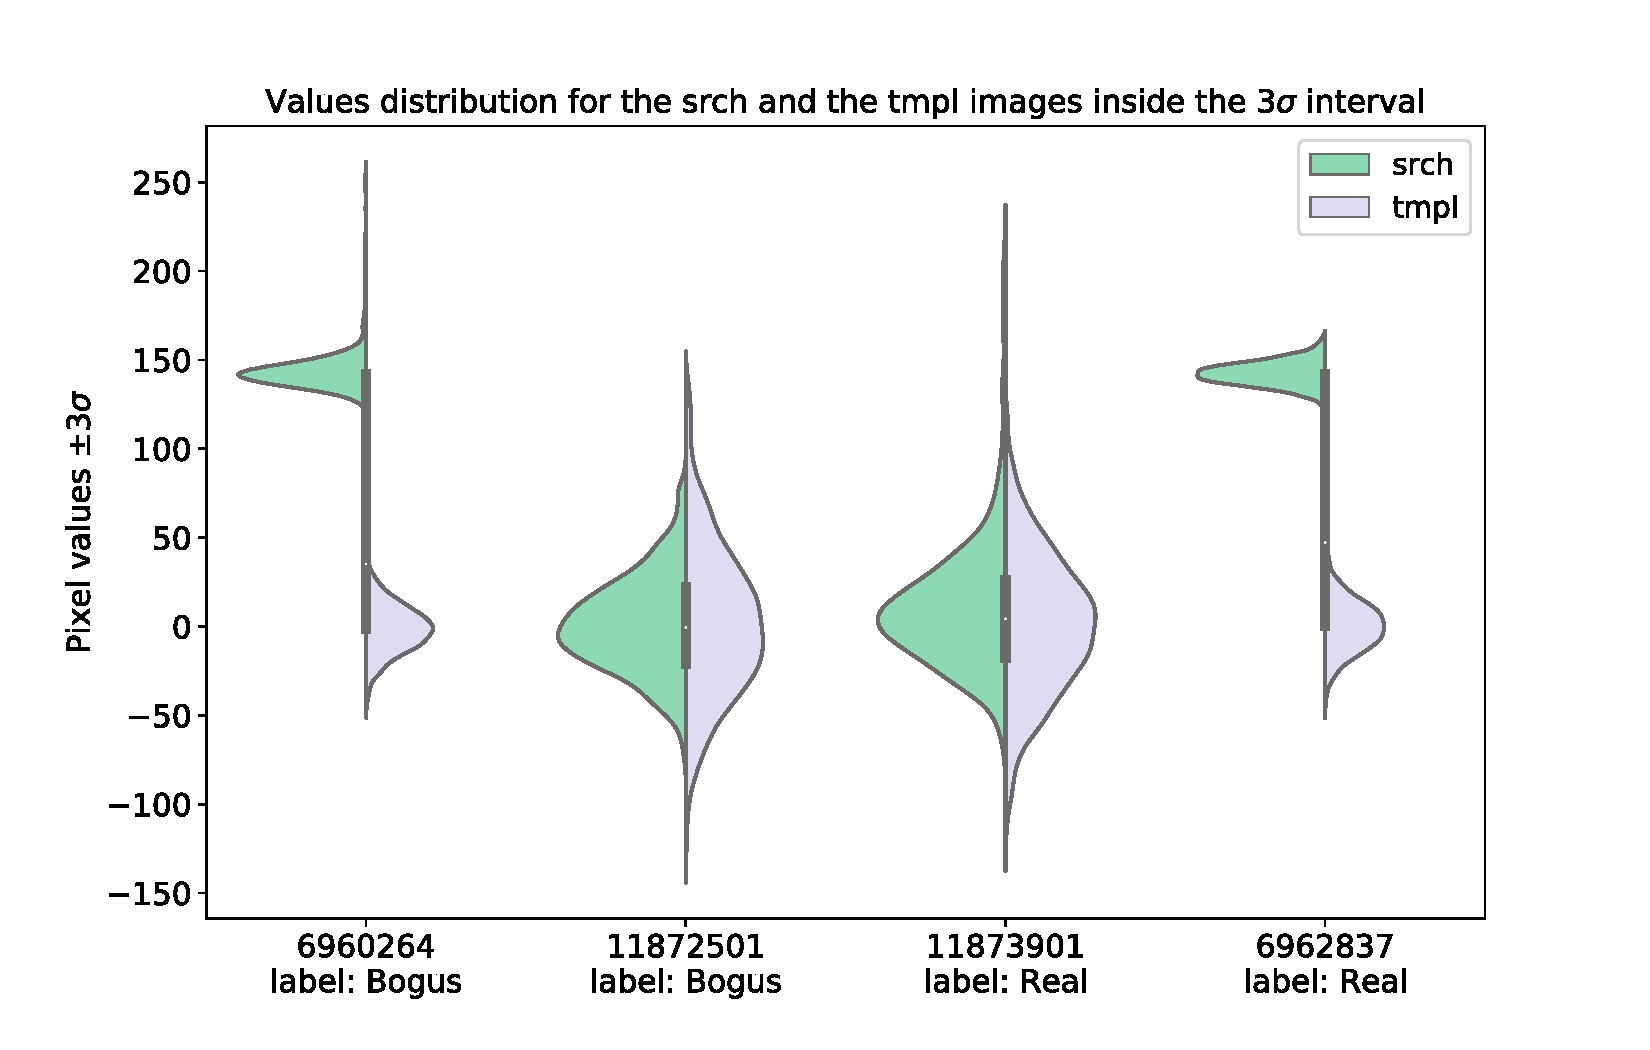
\includegraphics[width=0.6\linewidth]{
    figures/violin_plot.pdf}
    \caption{Violin plot of pixel values inside the $\mu \pm 3\sigma$ interval for \textit{srch} and \textit{temp} image of %Quantitative representation of 
    the data shown in \autoref{fig:examples_no_normalization} (before normalization). These values were scaled between $0$ and $1$. Left and right curve correspond to \textit{srch} and \textit{temp} distribution of values respectively. The distribution of values correspond to the same shown in \autoref{fig:histobeforenormalizarion} for \textit{srch} and \textit{temp}, the green and purple colors has its correspondence to \autoref{fig:histobeforenormalizarion}.}
    \label{fig:violinplot}
\end{figure*}



\begin{figure*}
    \centering
    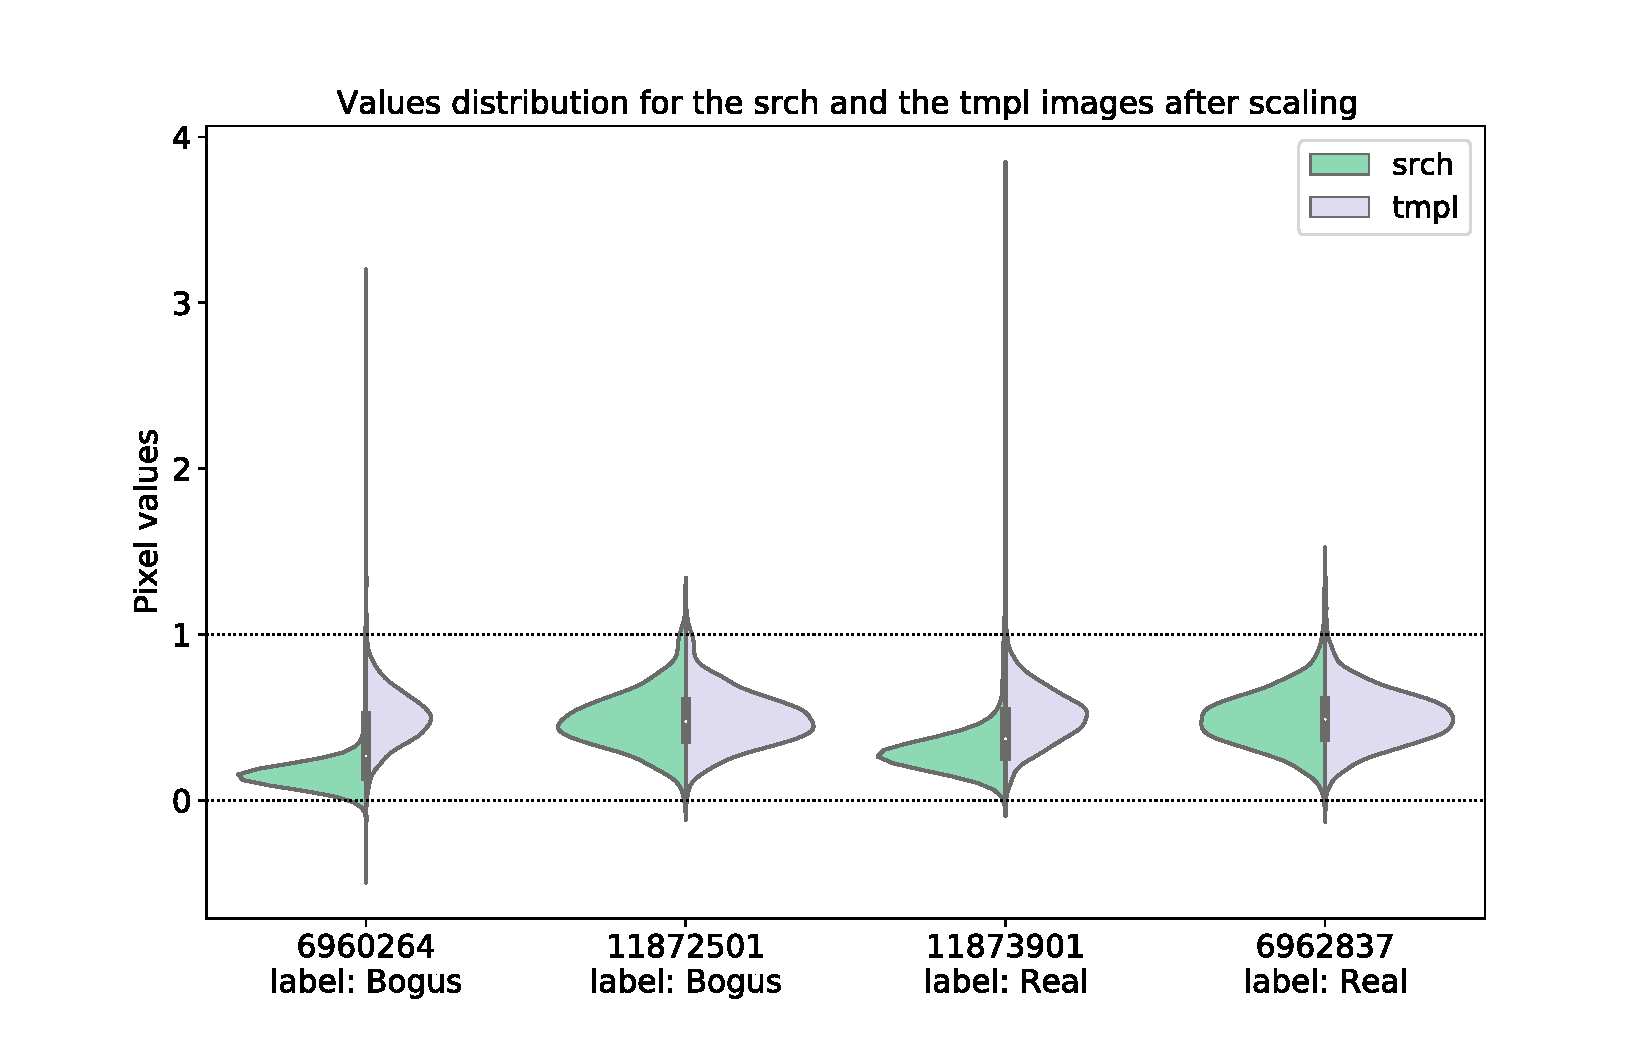
\includegraphics[width=0.6\linewidth]{
    figures/violin_plot_scaling.pdf}
    \caption{Violin plot of pixel values for \textit{srch} and \textit{temp} image of %Quantitative representation of 
    the data shown in \autoref{fig:examples_no_normalization} (after normalization). Values between the vertical lines in $0$ and $1$ were mapped to the values in \autoref{fig:violinplot}. Negative values and above $1$ correspond to the scaled values outside the $3\sigma$ clip. }
    \label{fig:violinplotscaling}
\end{figure*}

\clearpage


% \begin{itemize}
% \item \mintinline{c}/Conv2D/:
% % \subsubsection{\mintinline{c}/Conv2D/}
% According to the documentation of Convolutional layers in \url{https://keras.io/api/layers/convolution\_layers/convolution2d/}. The first parameter (\mintinline{c}/filter = 1 or 16 or 32 /) refers to the number of filters that the layer is going to learn. The outer layers learn less from the data than the inner layers. The second parameter (\mintinline{c}/kernel_size = [5,5]/) refers to the width and height of the filter that is multiplying the input data, the elements of the filter are the weights. The third parameter (\mintinline{c}/padding = "valid"/) define the way that the filter is going to sweep the input data, \mintinline{c}/"valid"/ refers that the operation between filter and input data is possible only if all the elements of the filters have a corresponding element in the input data. With this parameter the size of the output data is going to be smaller than the input. The latter parameters used here is the \mintinline{c}/activation = "relu"/,``Rectified Linear Unit''. The output data, know as feature map, is pass through the activation function to get the output layer.
% %to get the bias. 
% % The \mintinline{c}/"relu"/ function is defined as:
% % \begin{equation*}
% % ReLU = 
% % \begin{cases}
% %     0, & x\le0\\
% %     x, & x>0
% % \end{cases}
% % \end{equation*}
% %The ReLU is an efficient activation function that improves the performance of the Neural Network. [\cite{DBLP:journals/corr/abs-1803-08375, 10.5555/2999134.2999257, Dieleman_2015}]

% %\item \mintinline{c}/Conv2D/:
% %Reduces the size of the output given in \mintinline{c}/Conv2D/ by a given matrix size, selecting the maximum value of the window where the pool matrix fit within the matrix output of the \mintinline{c}/Conv2D/. The size reduction is done by applying an aggregation function to the output of the previous layer, in this case to choose the maximum value within a specific windows across all the output, small translation could lead to the same maximum values. This layer add an approximately invariance on small translations. \citep{Gieseke_2017}

% \item \mintinline{c}/Dropout/:
% Eliminates randomly output values of the previous layer, the CNN model would not learn features that are not relevant to unseen data. In this way a better performance on the training data, compared to the validation or testing data would be avoided, the called \textit{overfitting}. The model would be able to predicted successfully with the same or similar rate in both data sets. [\cite{Dieleman_2015, Gieseke_2017}]

% \item \mintinline{c}/Flatten/:
% Reduces the dimensions of the data to be a one dimension array.

% \item \mintinline{c}/Dense/:
% Make the previous layer all fully connected with the next layer.

% \end{itemize}


% \appendix 

\section{Detailed architecture of \diabased\ and \nodia\ models}
\label{sec:appendixb}





We designed a network of 12 layers using \mintinline{c}/tensorflow.keras/in python, for the \diabased\ case as follows:
\vspace{1cm}

%\begin{figure*}[H]
\begin{minted}{python}
layer1 = keras.layers.Conv2D(16, kernel_size=(5, 5), padding="valid", activation="relu", 
                             input_shape=(51,153,1))
layer2 = keras.layers.MaxPooling2D((2, 2), strides=2)
layer3 = keras.layers.Dropout(0.4)
layer4 = keras.layers.Conv2D(32, kernel_size=(5, 5), padding="valid", activation="relu")
layer5 = keras.layers.MaxPooling2D((2, 2), strides=2)
layer6 = keras.layers.Dropout(0.4)
layer7 = keras.layers.Conv2D(64, kernel_size=(5, 5), padding="valid", activation="relu")
layer8 = keras.layers.MaxPooling2D((2, 2), strides=2)
layer9 = keras.layers.Dropout(0.4)
layer10 = keras.layers.Flatten()
layer11 = keras.layers.Dense(32, activation="relu")
layer12 = keras.layers.Dense(2, activation="softmax")
\end{minted}
%\end{figure*}
\FloatBarrier

\vspace{1cm}

\noindent and a network of 11 layers using  \mintinline{c}/tensorflow.keras/in python, for the \nodia\ case as follows:
\vspace{1cm}

\begin{minted}{python}
layer1 = keras.layers.Conv2D(1, kernel_size=(7, 7), padding="valid", activation="relu", 
                             input_shape=(51,102,1))
layer2 = keras.layers.MaxPooling2D((2, 2), strides=2)
layer3 = keras.layers.Conv2D(16, kernel_size=(3, 3), padding="valid", activation="relu")
layer4 = keras.layers.MaxPooling2D((2, 2), strides=2)
layer5 = keras.layers.Dropout(0.4)
layer6 = keras.layers.Conv2D(32, kernel_size=(3, 3), padding="valid", activation="relu")
layer7 = keras.layers.MaxPooling2D((2, 2), strides=2)
layer8 = keras.layers.Dropout(0.4)
layer9 = keras.layers.Flatten()
layer10 = keras.layers.Dense(32, activation="relu")
layer11 = keras.layers.Dense(2, activation="softmax")
\end{minted}
To compile the models we used the optimizer \mintinline{c}/SGD/ (stochastic gradient descent) with a \mintinline{c}/learning_rate=0.01/ the \mintinline{c}/"sparse_categorical_crossentropy"/ loss function and the \mintinline{c}/"accuracy"/ metric. Our models are available in a dedicated GitHub repository \footnote{\url{https://github.com/taceroc/DIA_noDIA}.}

\clearpage

% \appendix 
\section{Saliency maps for various transients}

\label{sec:appendixc}




We include a series of saliency maps  in the following 8 figures. Several interesting behavioral patterns can be observed. The figures are organized by model and by classification as follows: TN ---\autoref{fig:saliency_3id_contour} and \autoref{fig:saliency_nodia3id_contour}---, TP ---\autoref{fig:saliency_dia3id_TP} and \autoref{fig:tpndia}---, FN \autoref{fig:saliency_dia3id_FN} and \autoref{fig:fnndia}–––, and FP ---\autoref{fig:saliency_dia3id_FP} and \autoref{fig:fpndia}.

In  \autoref{fig:saliency_3id_contour} and \autoref{fig:saliency_nodia3id_contour} we include the transient's contours overplotted onto the saliency maps for the \diabased\ and \nodia\ model respectively to guide the reader's eye. 
% We note a few intriguing features and speculate on their meaning. In \autoref{fig:saliency_3id_contour}A, a dipole, the important pixels are located off-center, in correspondence to the dark portion of the dipole (althought we note that this classification is incorrect \fed{can you add a dipole with correct classification?}). 
Notice the offset of the \diabased\ model's focus in  \autoref{fig:saliency_3id_contour}A with respect to the transient: the model is principally inspecting the \diff\ and \temp\ at the location corresponding to the bright patch in the \diff.
In  \autoref{fig:saliency_3id_contour}C a correctly predicted ``bogus'', characterized by a very tight dipole probably arising from a poorly centered DIA, the saliency map inspect the \temp\ and even seem to reproduce traditional aperture photometry, with pixel values measured at the core of the transients, and in the sky surrounding the transients, but away from the tails of the bright pixels cluster. The behavior is principally different for the same transients when they are inspected, and also correctly predicted, by the \nodia\ model (\autoref{fig:saliency_nodia3id_contour}): the focus of the model is in all three cases away from the transients, and shifted to the surrounding: the model is learning the transients' context and extracting information to enable the comparison of \temp\ and \diff\ (essentially, to enable the image differencing). This behavior is generally seen throughout all examples in the following figures. In addition, for each figure we highlight potential reasons for failed predictions, and potential inaccuracies in the labeling that may lead to an artificial lowering of our measured accuracy.



\begin{figure*}
    \centering
    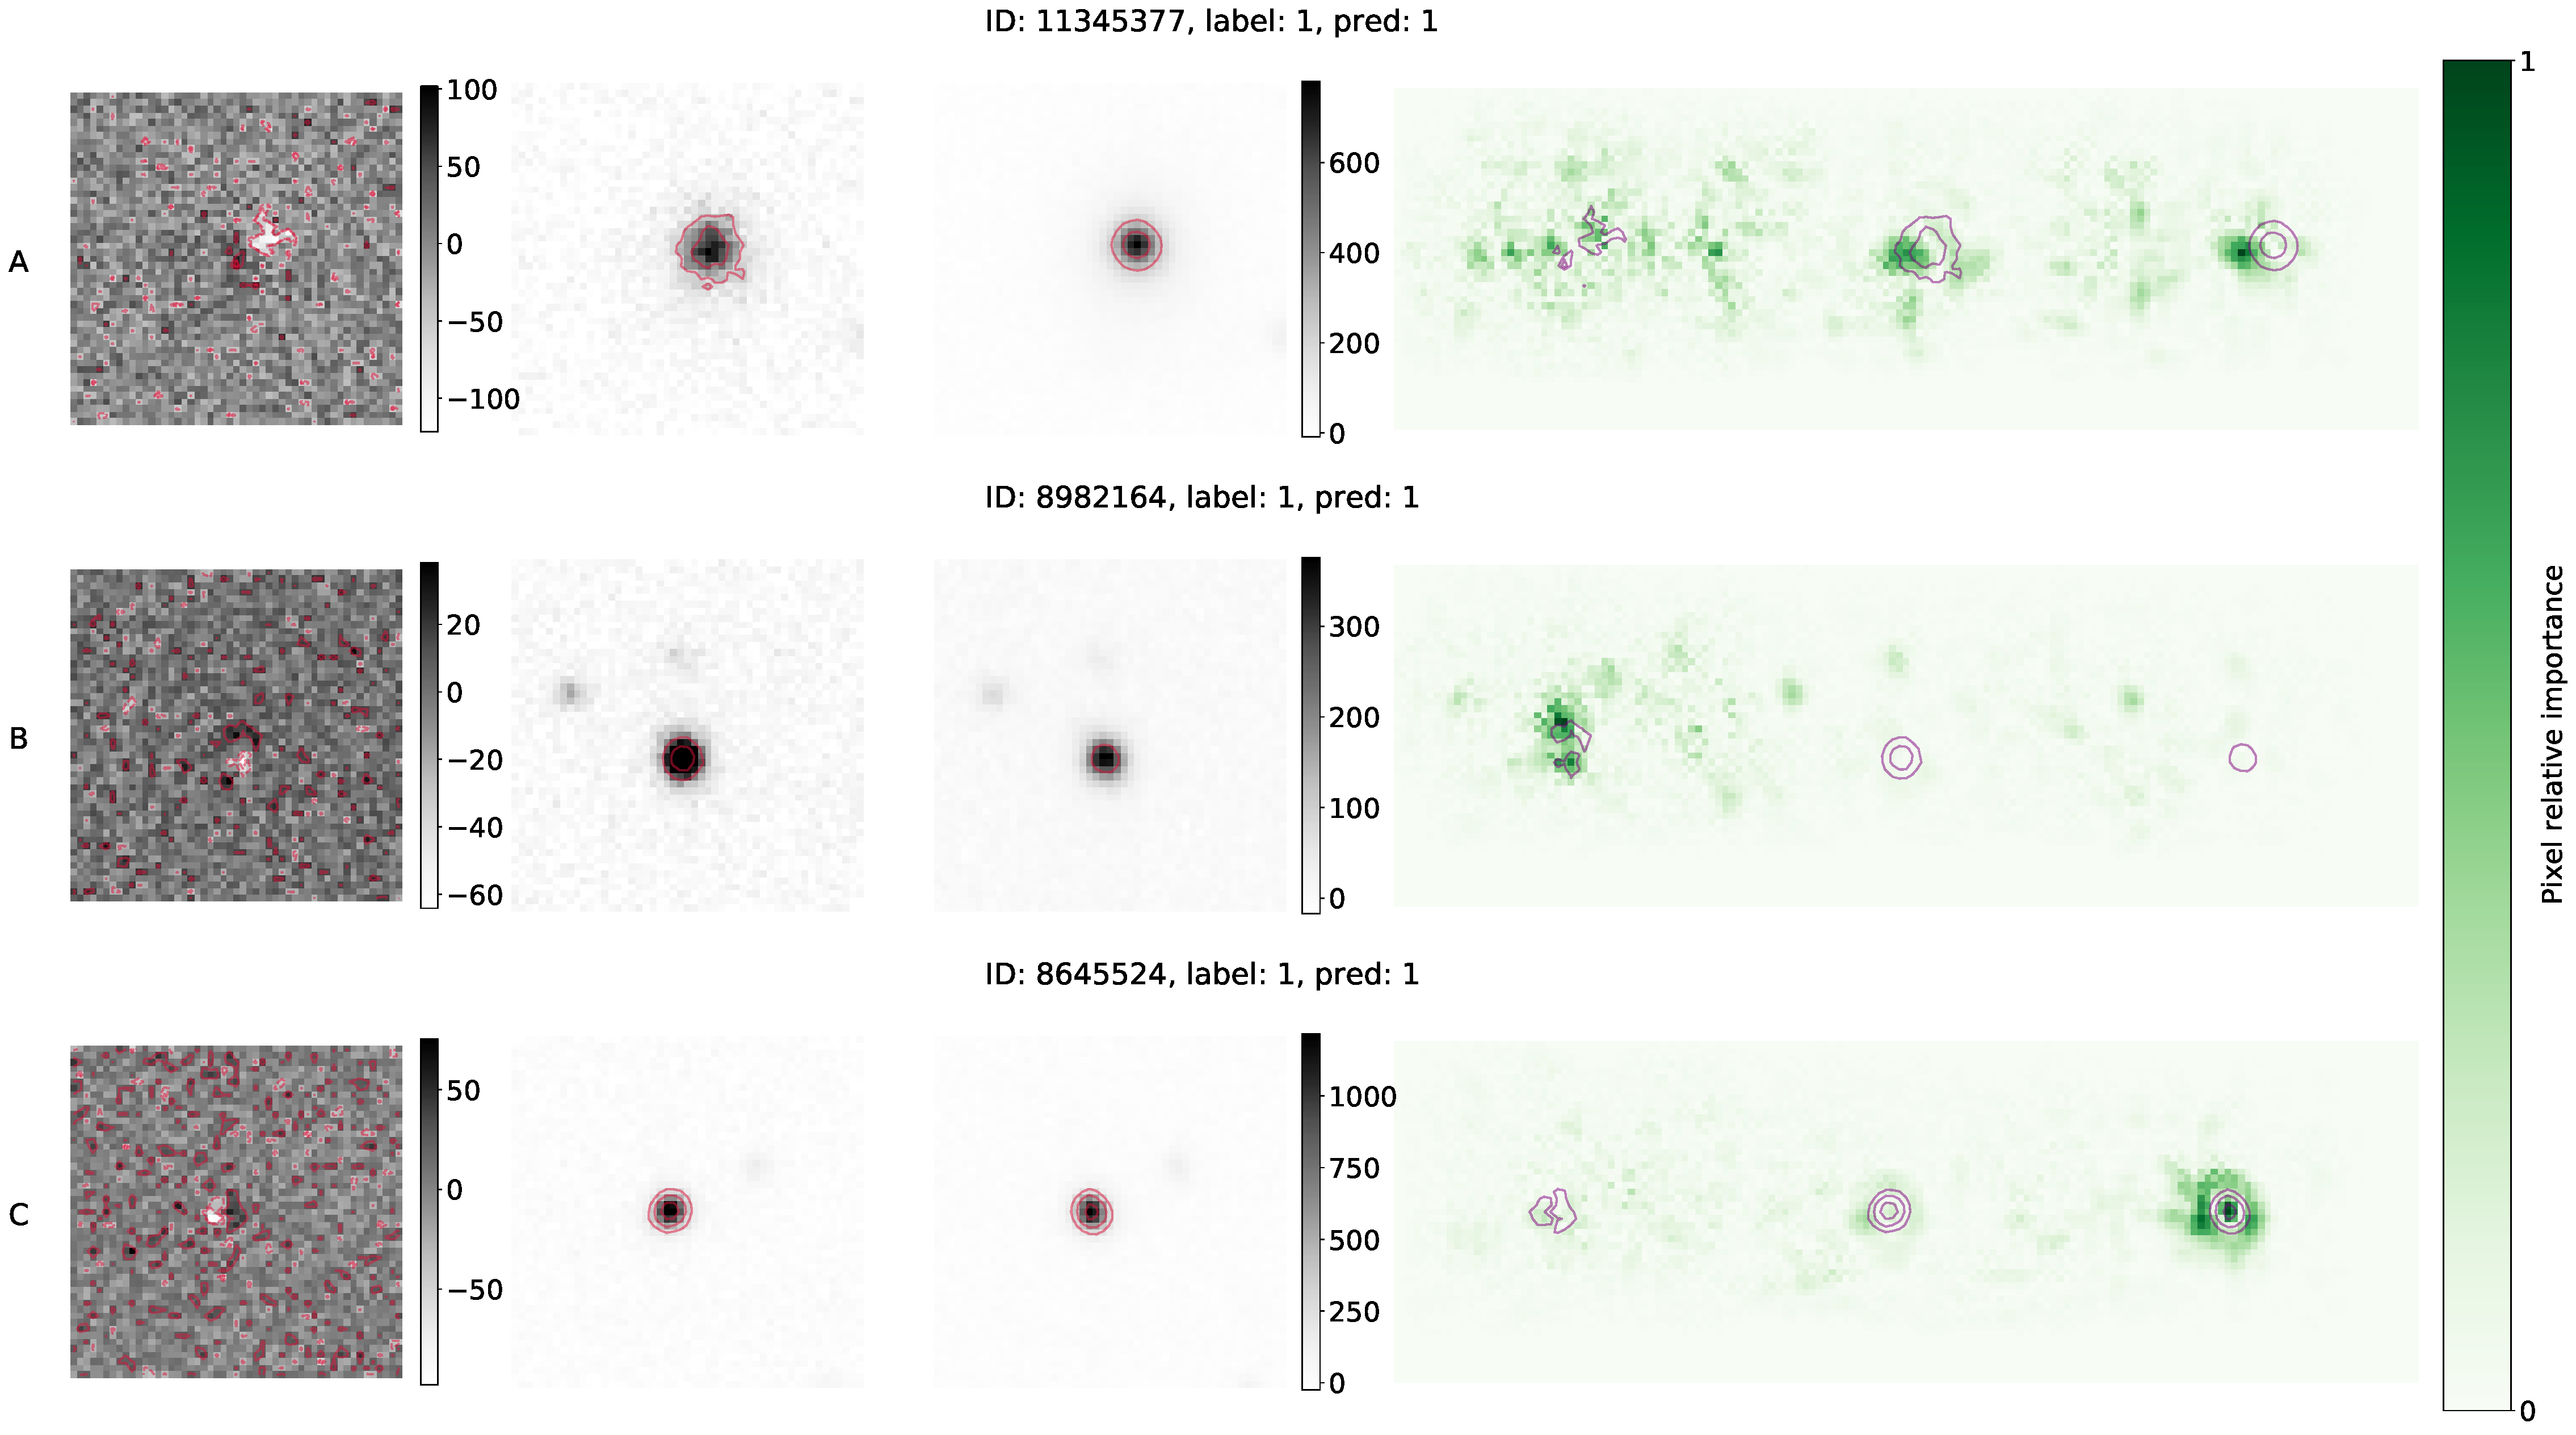
\includegraphics[width=0.85\linewidth]{
    figures/saliency_plot_3exam_contou_cheating.pdf}
    \caption{Transients (\diff-\search-\temp) and their respective saliency map for \diabased\ model True Negative predictions (correctly identified ``bogus'').  Contour plot of light intensity from the original images are overplotted, delineating the bright sources. In panel A: $I_\diff \sim 0.4$; B: $I_\diff\sim0.69$ and C $I_\temp\sim0.42$. In panel C, the saliency for the \temp\ portion of the image looks strikingly similar to the selection of pixels that is made in aperture photometry, with pixel values considered in the core of the source, ignored in a region immediately around the source, and again considered farther out to calculate the source's background. This figure is further discussed in \hyperref[sec:appendixc]{Appendix C}.}
    \label{fig:saliency_3id_contour}

    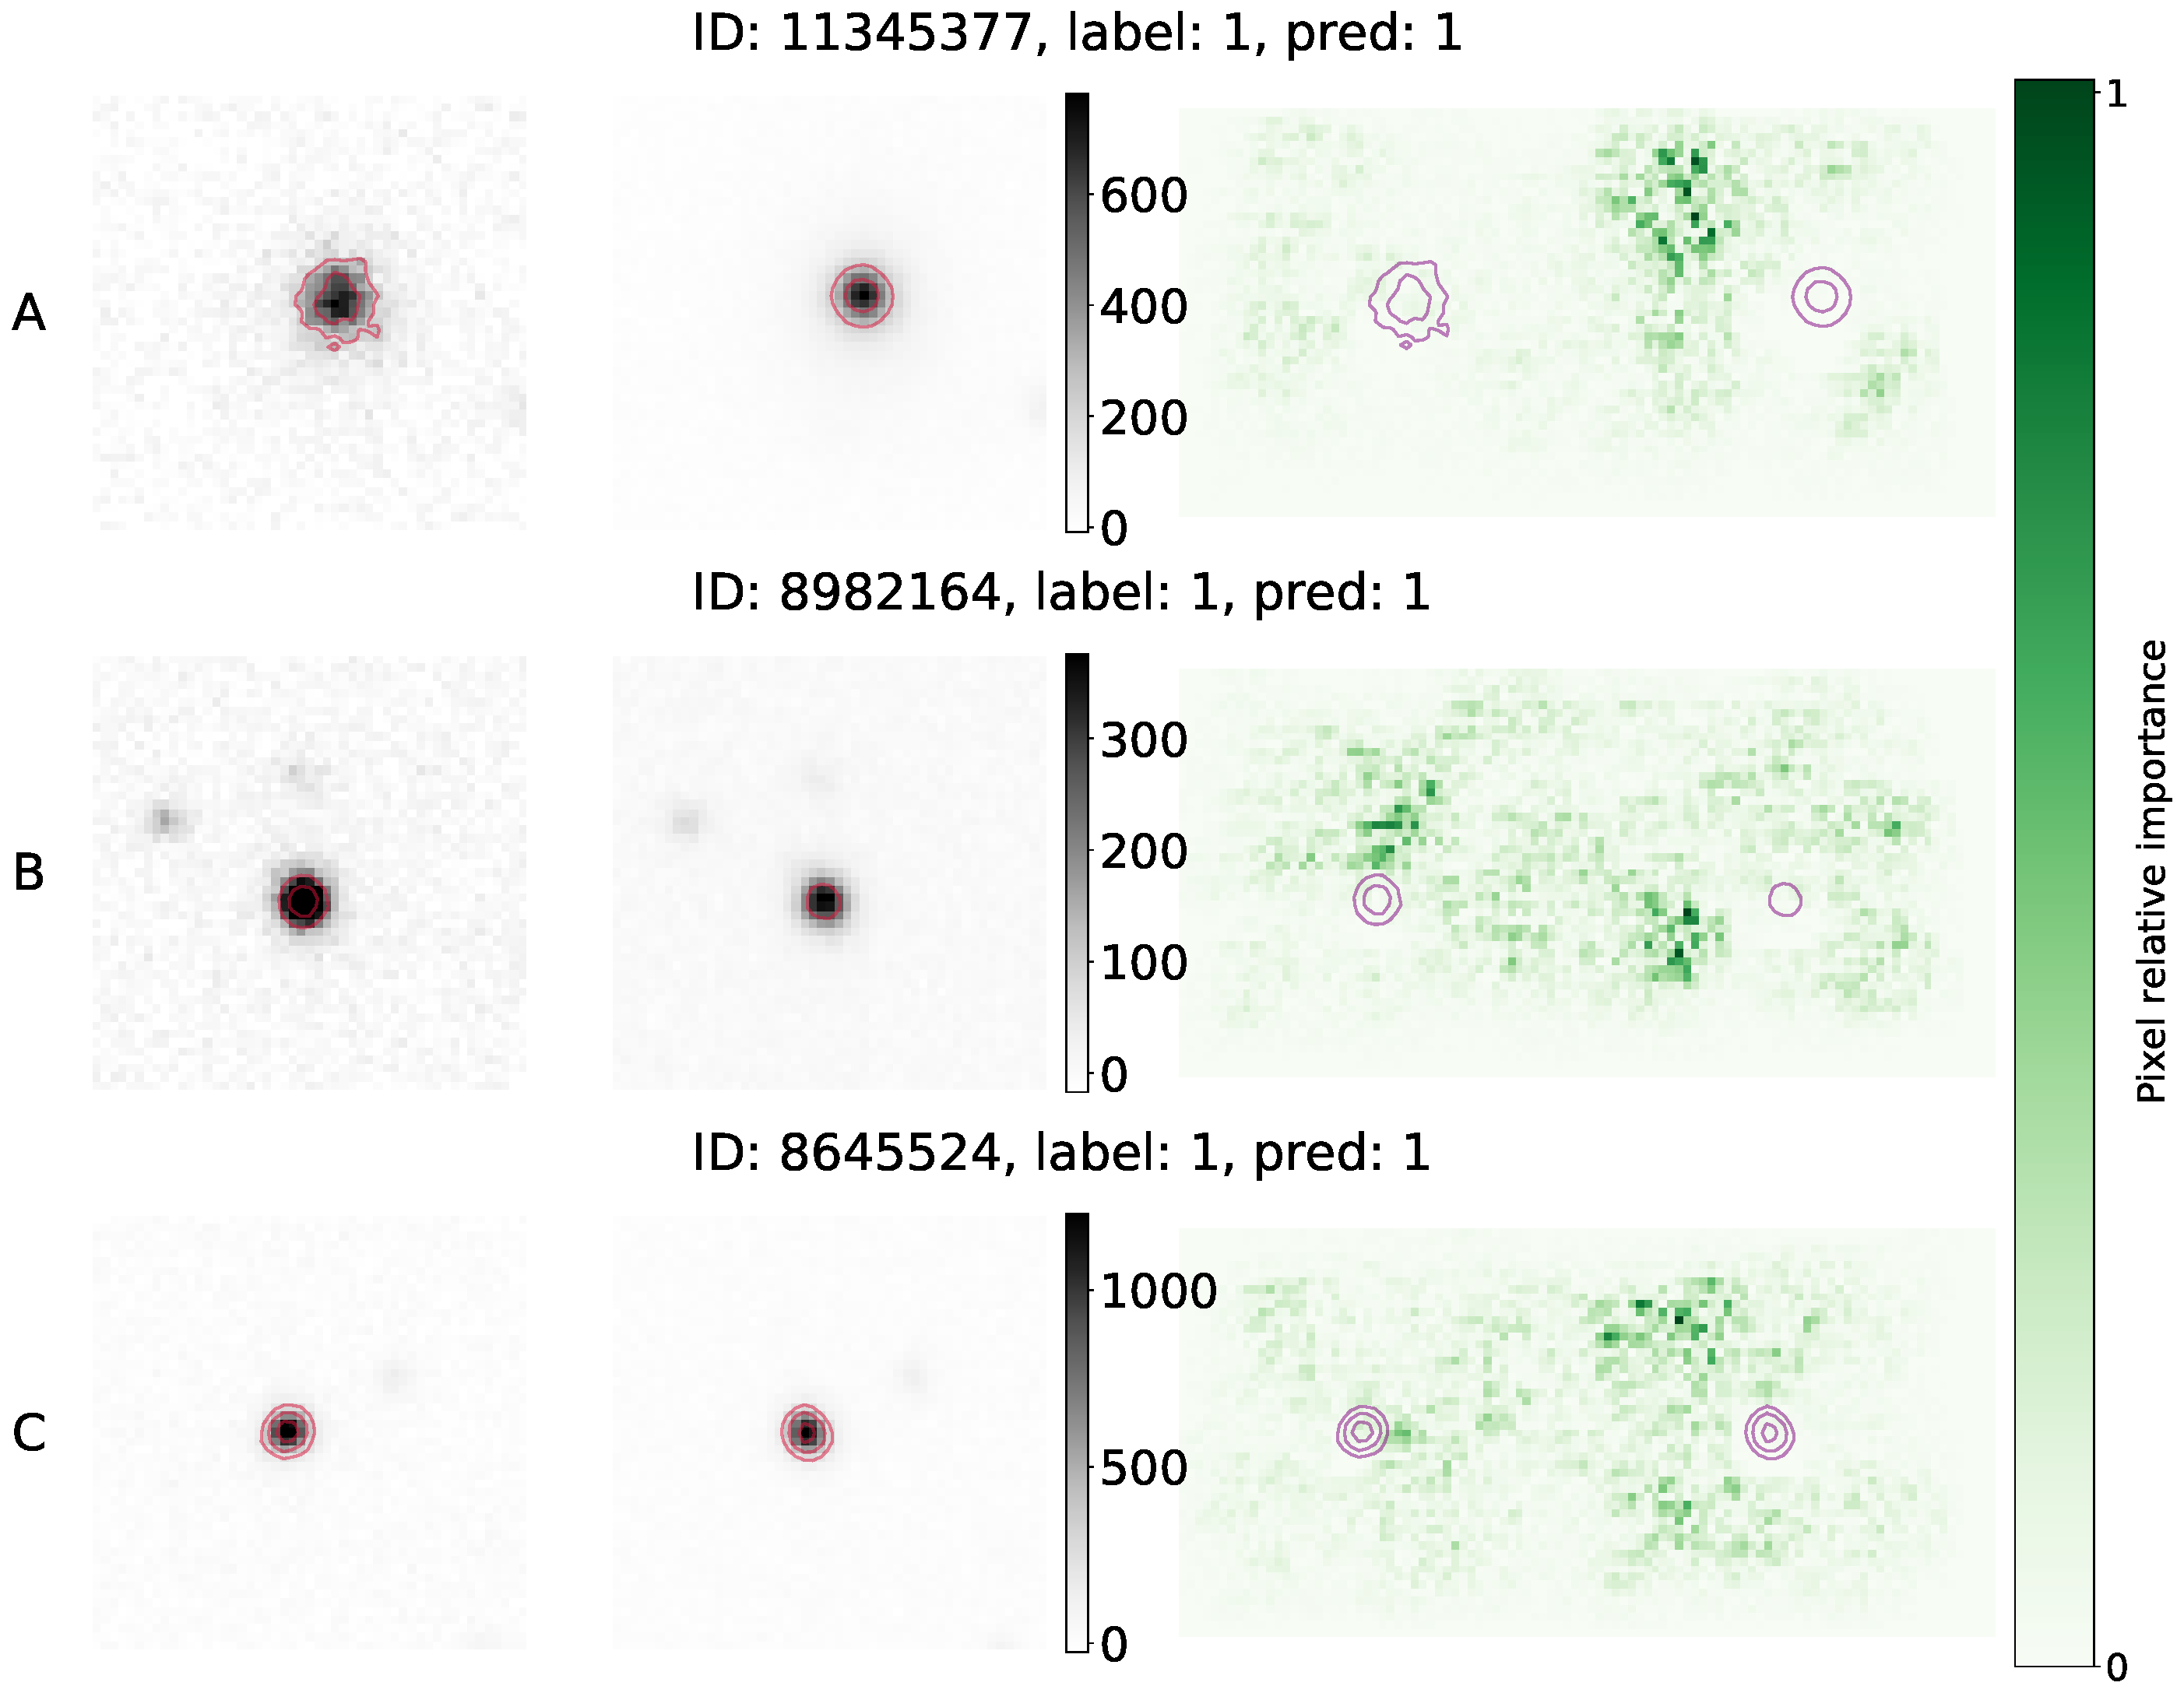
\includegraphics[width=0.65\linewidth]{
    figures/saliency_plot_noDIA3exam.pdf}
    \caption{The same transients (\search-\temp) shown in \autoref{fig:saliency_3id_contour} and their respective saliency maps for \nodia\ model True Negatives (correctly identified ``bogus'').  Important pixels are found at nearly all locations in the image, rather than in a small region around the center. The model needs to learn properties of the image at large to enable a comparison of the \temp\ and \diff.  This figure is further discussed in \hyperref[sec:appendixc]{Appendix C}.}
    \label{fig:saliency_nodia3id_contour}
\end{figure*}


\clearpage
\begin{figure*}
    \centering
    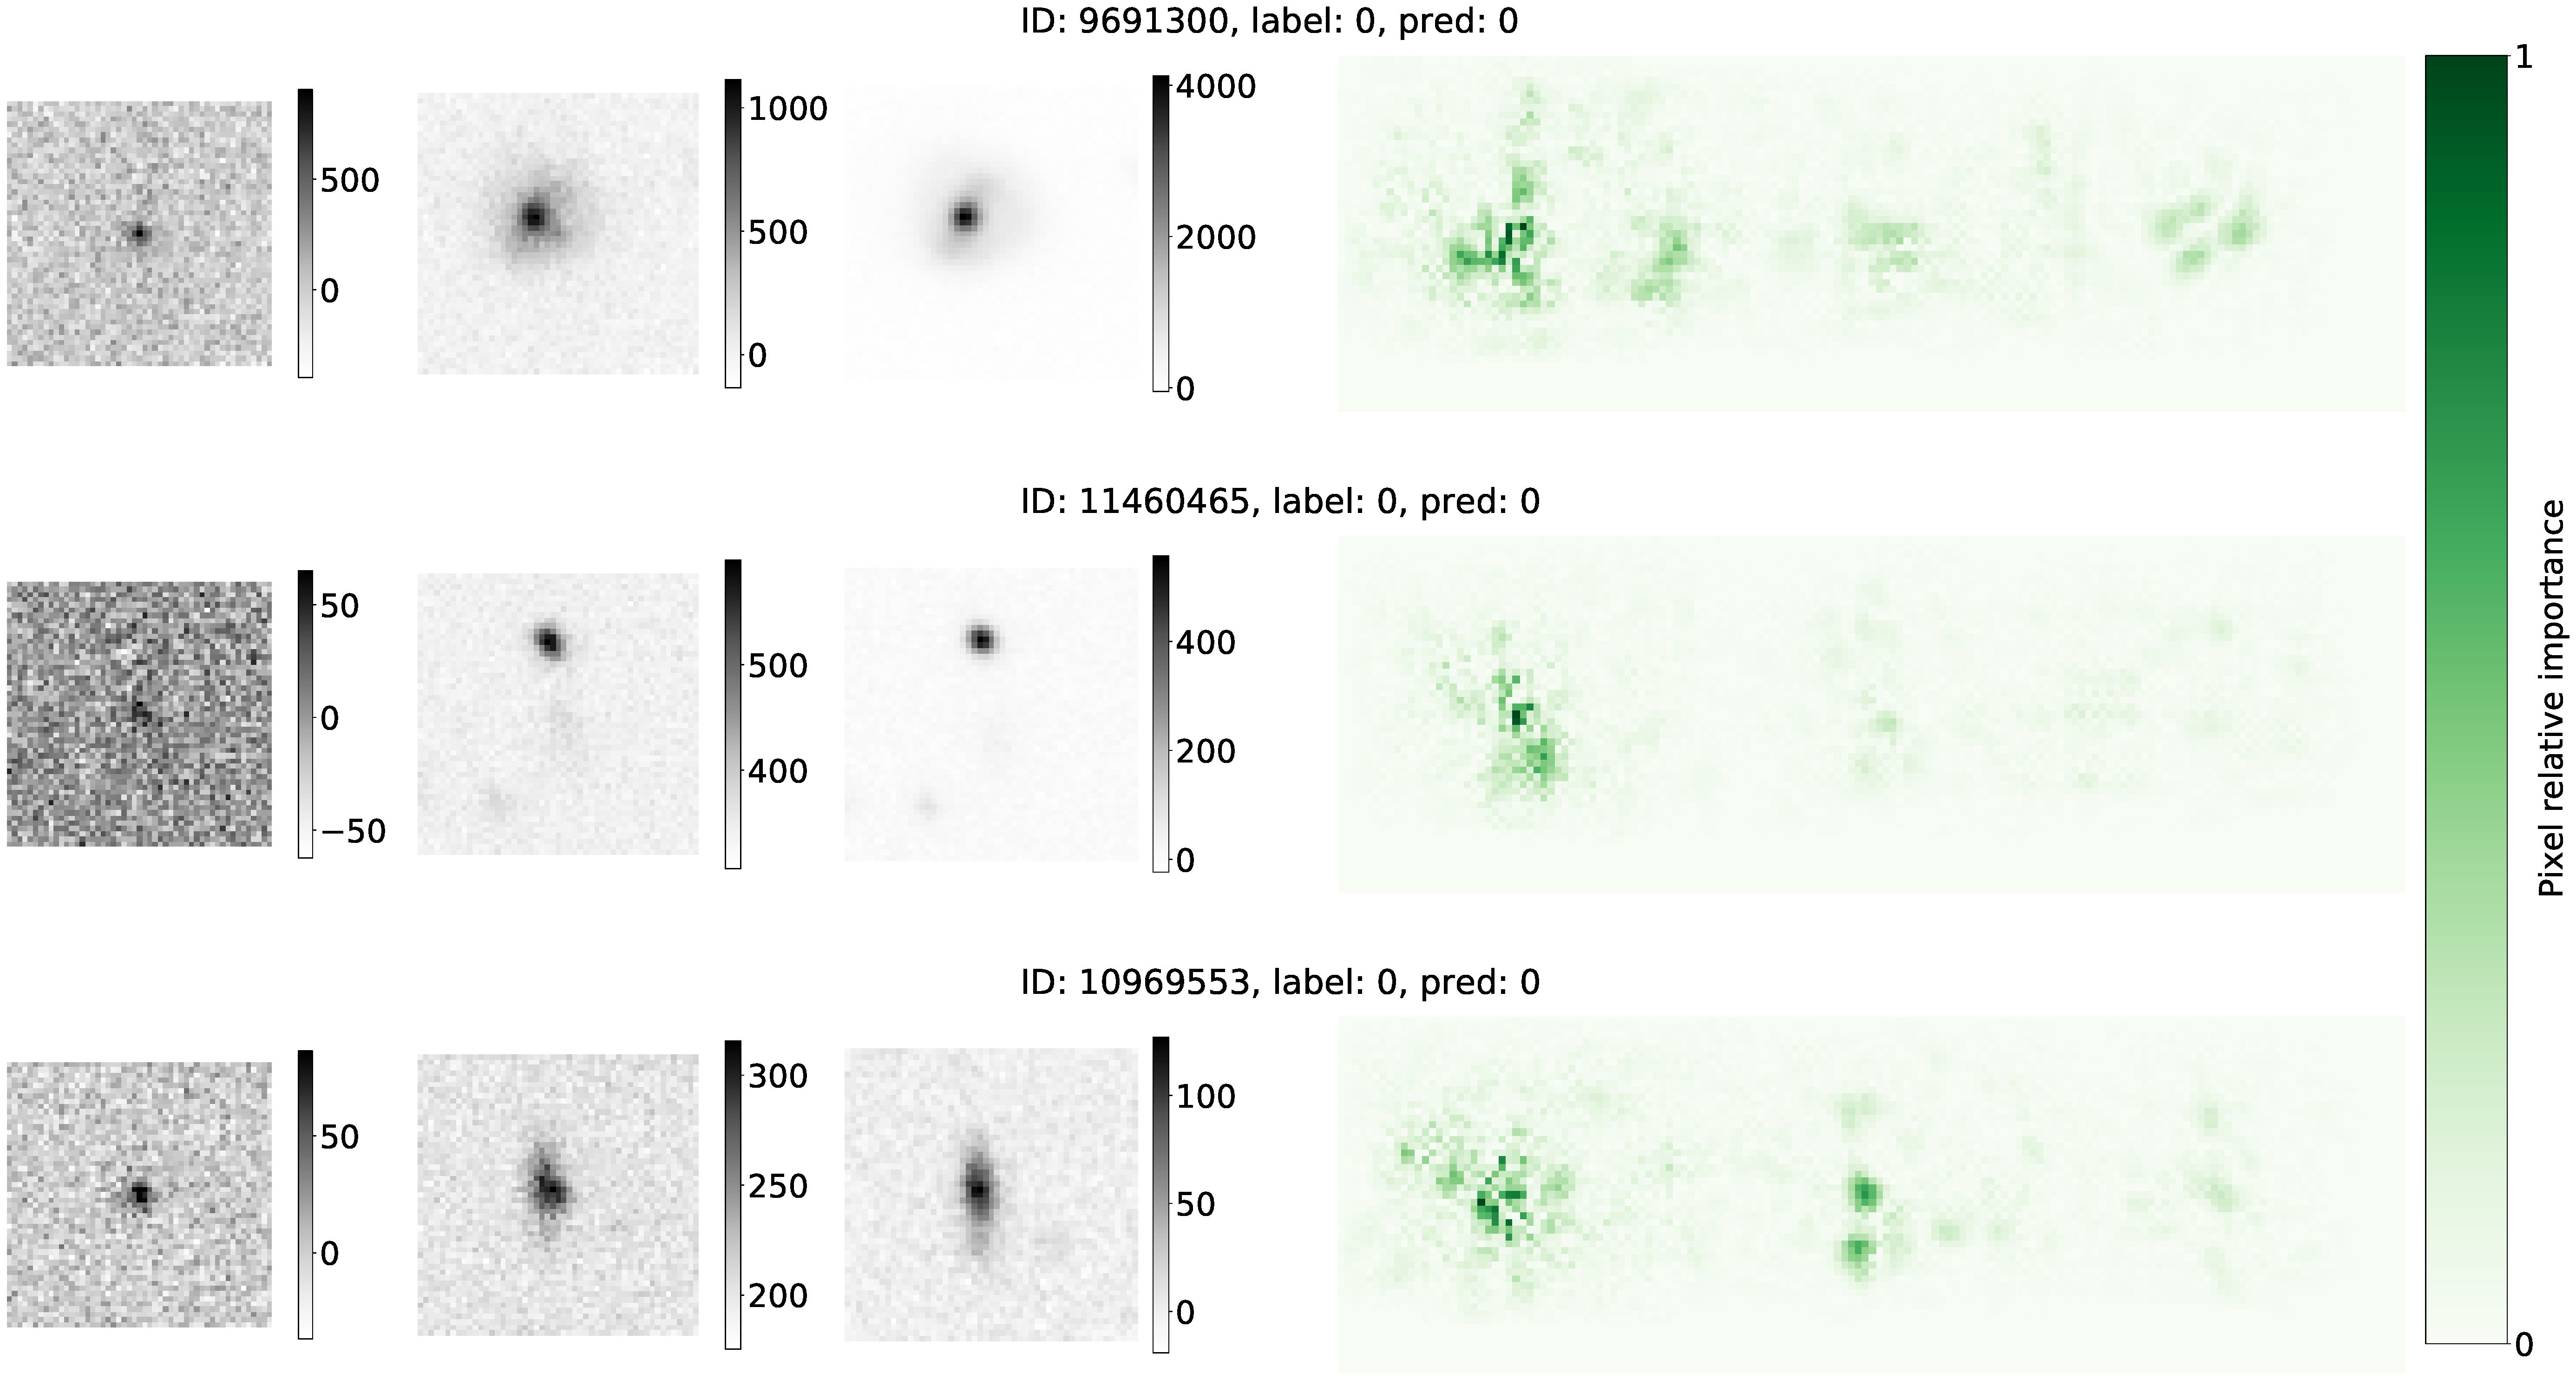
\includegraphics[width=0.8\linewidth]{
    figures/saliency_plot_other3-see64.pdf}
    
    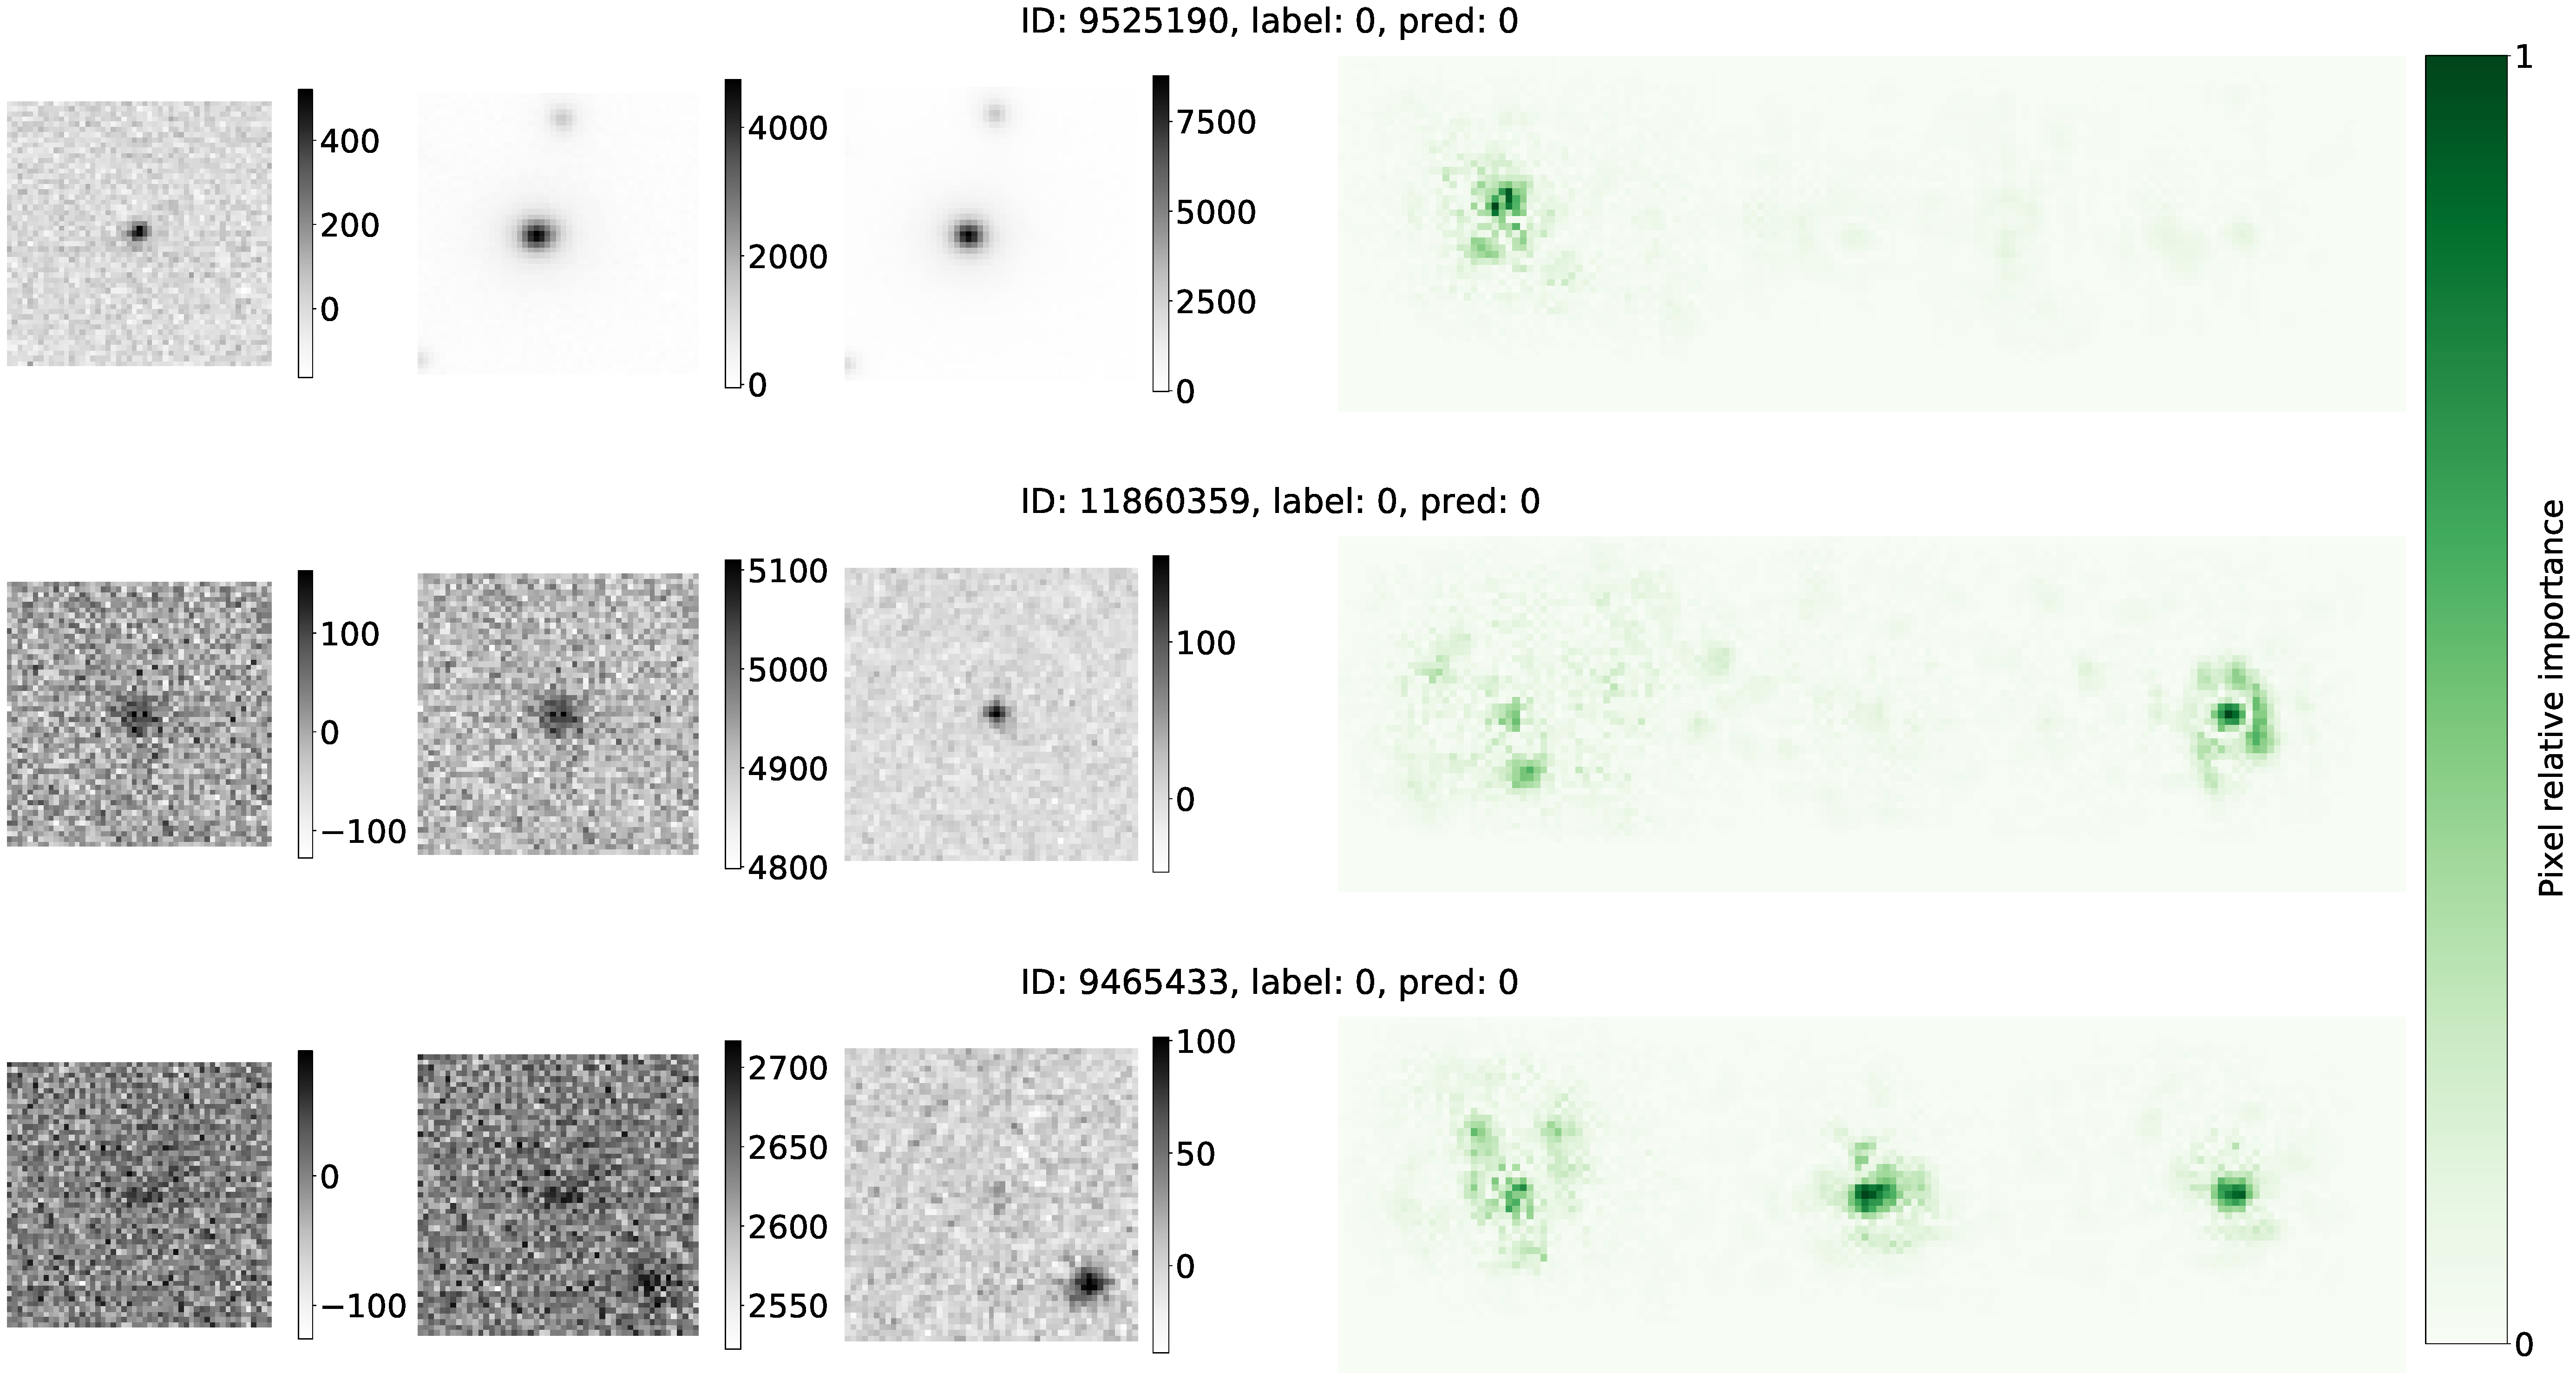
\includegraphics[width=0.8\linewidth]{
    figures/saliency_plot_other3-see109.pdf}
    \caption{Transients (\diff-\search-\temp) and their respective saliency map  for \diabased\ model True Positives  (correctly identified ``real'' astrophysical transients). The important pixels are generally found in the \diff\ portion of the image for the \diabased\ model, as discussed in \autoref{sec:results}, but there are exceptions: here we show several cases of True Positives (real transients) classifications where the component of the image that was principally leveraged by the model was the \diff\ (the leftmost third) but two cases where the \nodia\ relied principally on the \search\ and/or \temp\ (bottom two panels).}
    \label{fig:saliency_dia3id_TP}
\end{figure*}


\begin{figure*}
    \centering
    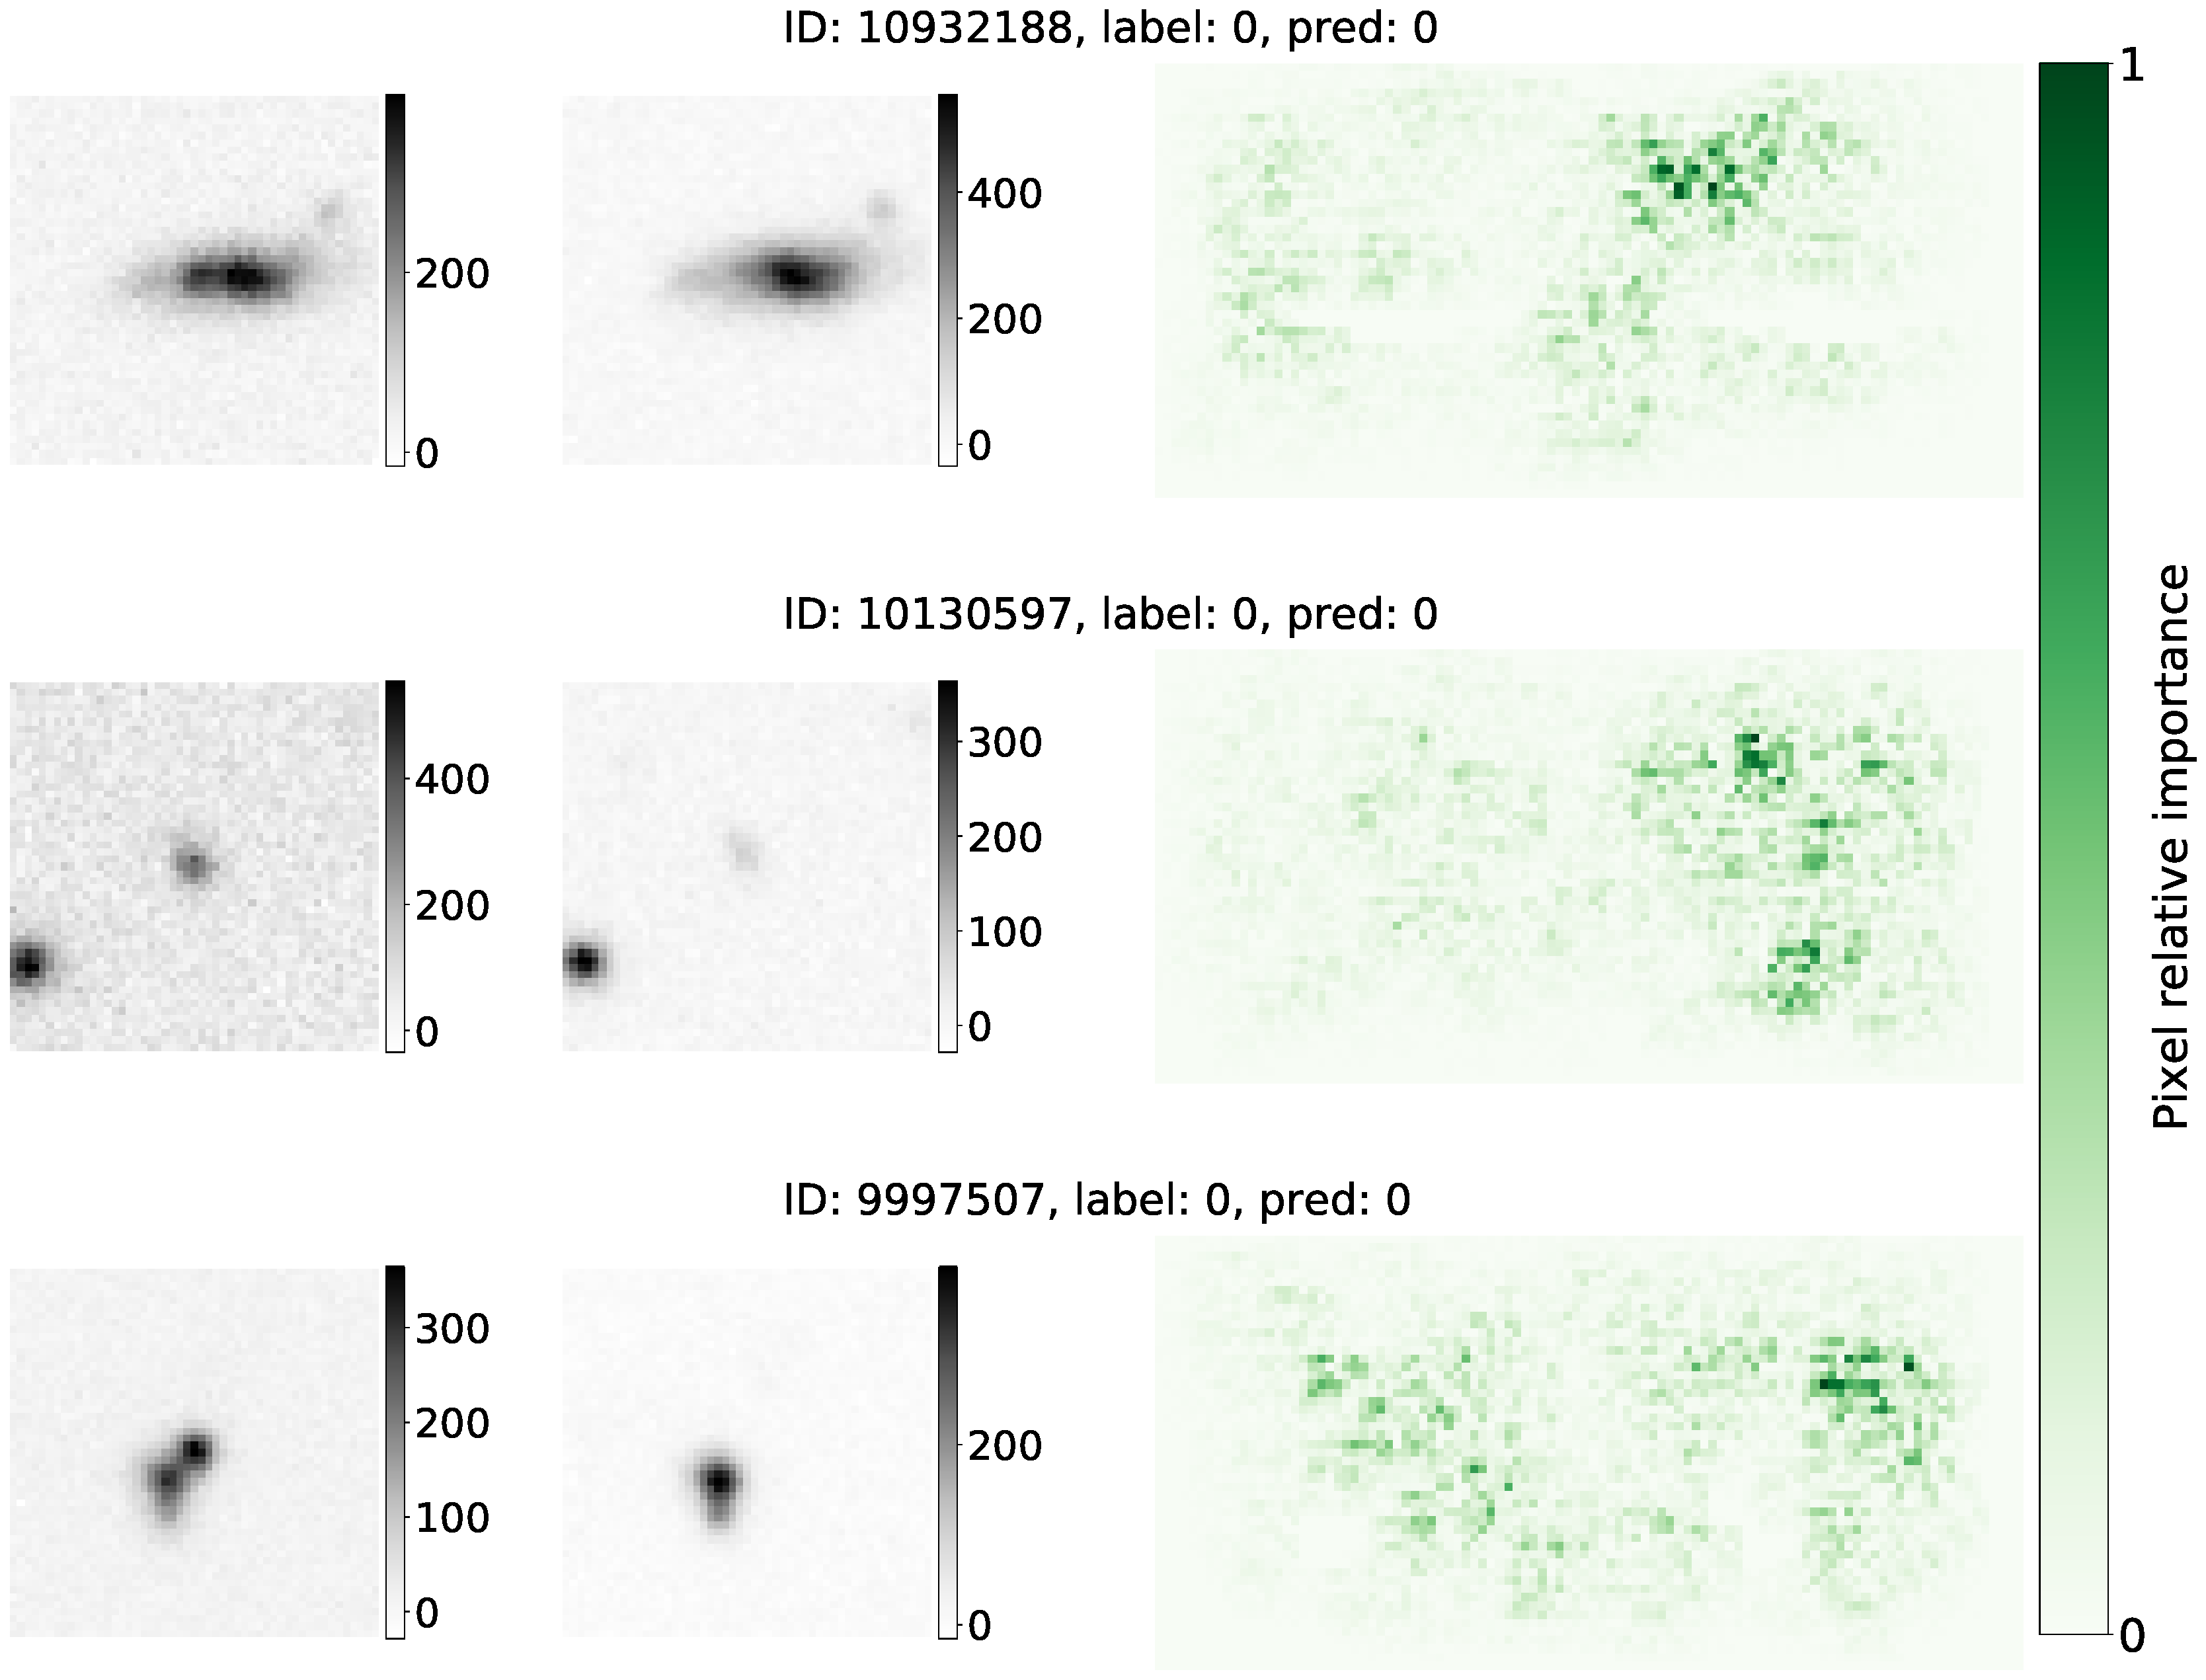
\includegraphics[width=0.8\linewidth]{
    figures/saliency_plot_other3nodiaTP-see766.pdf}
    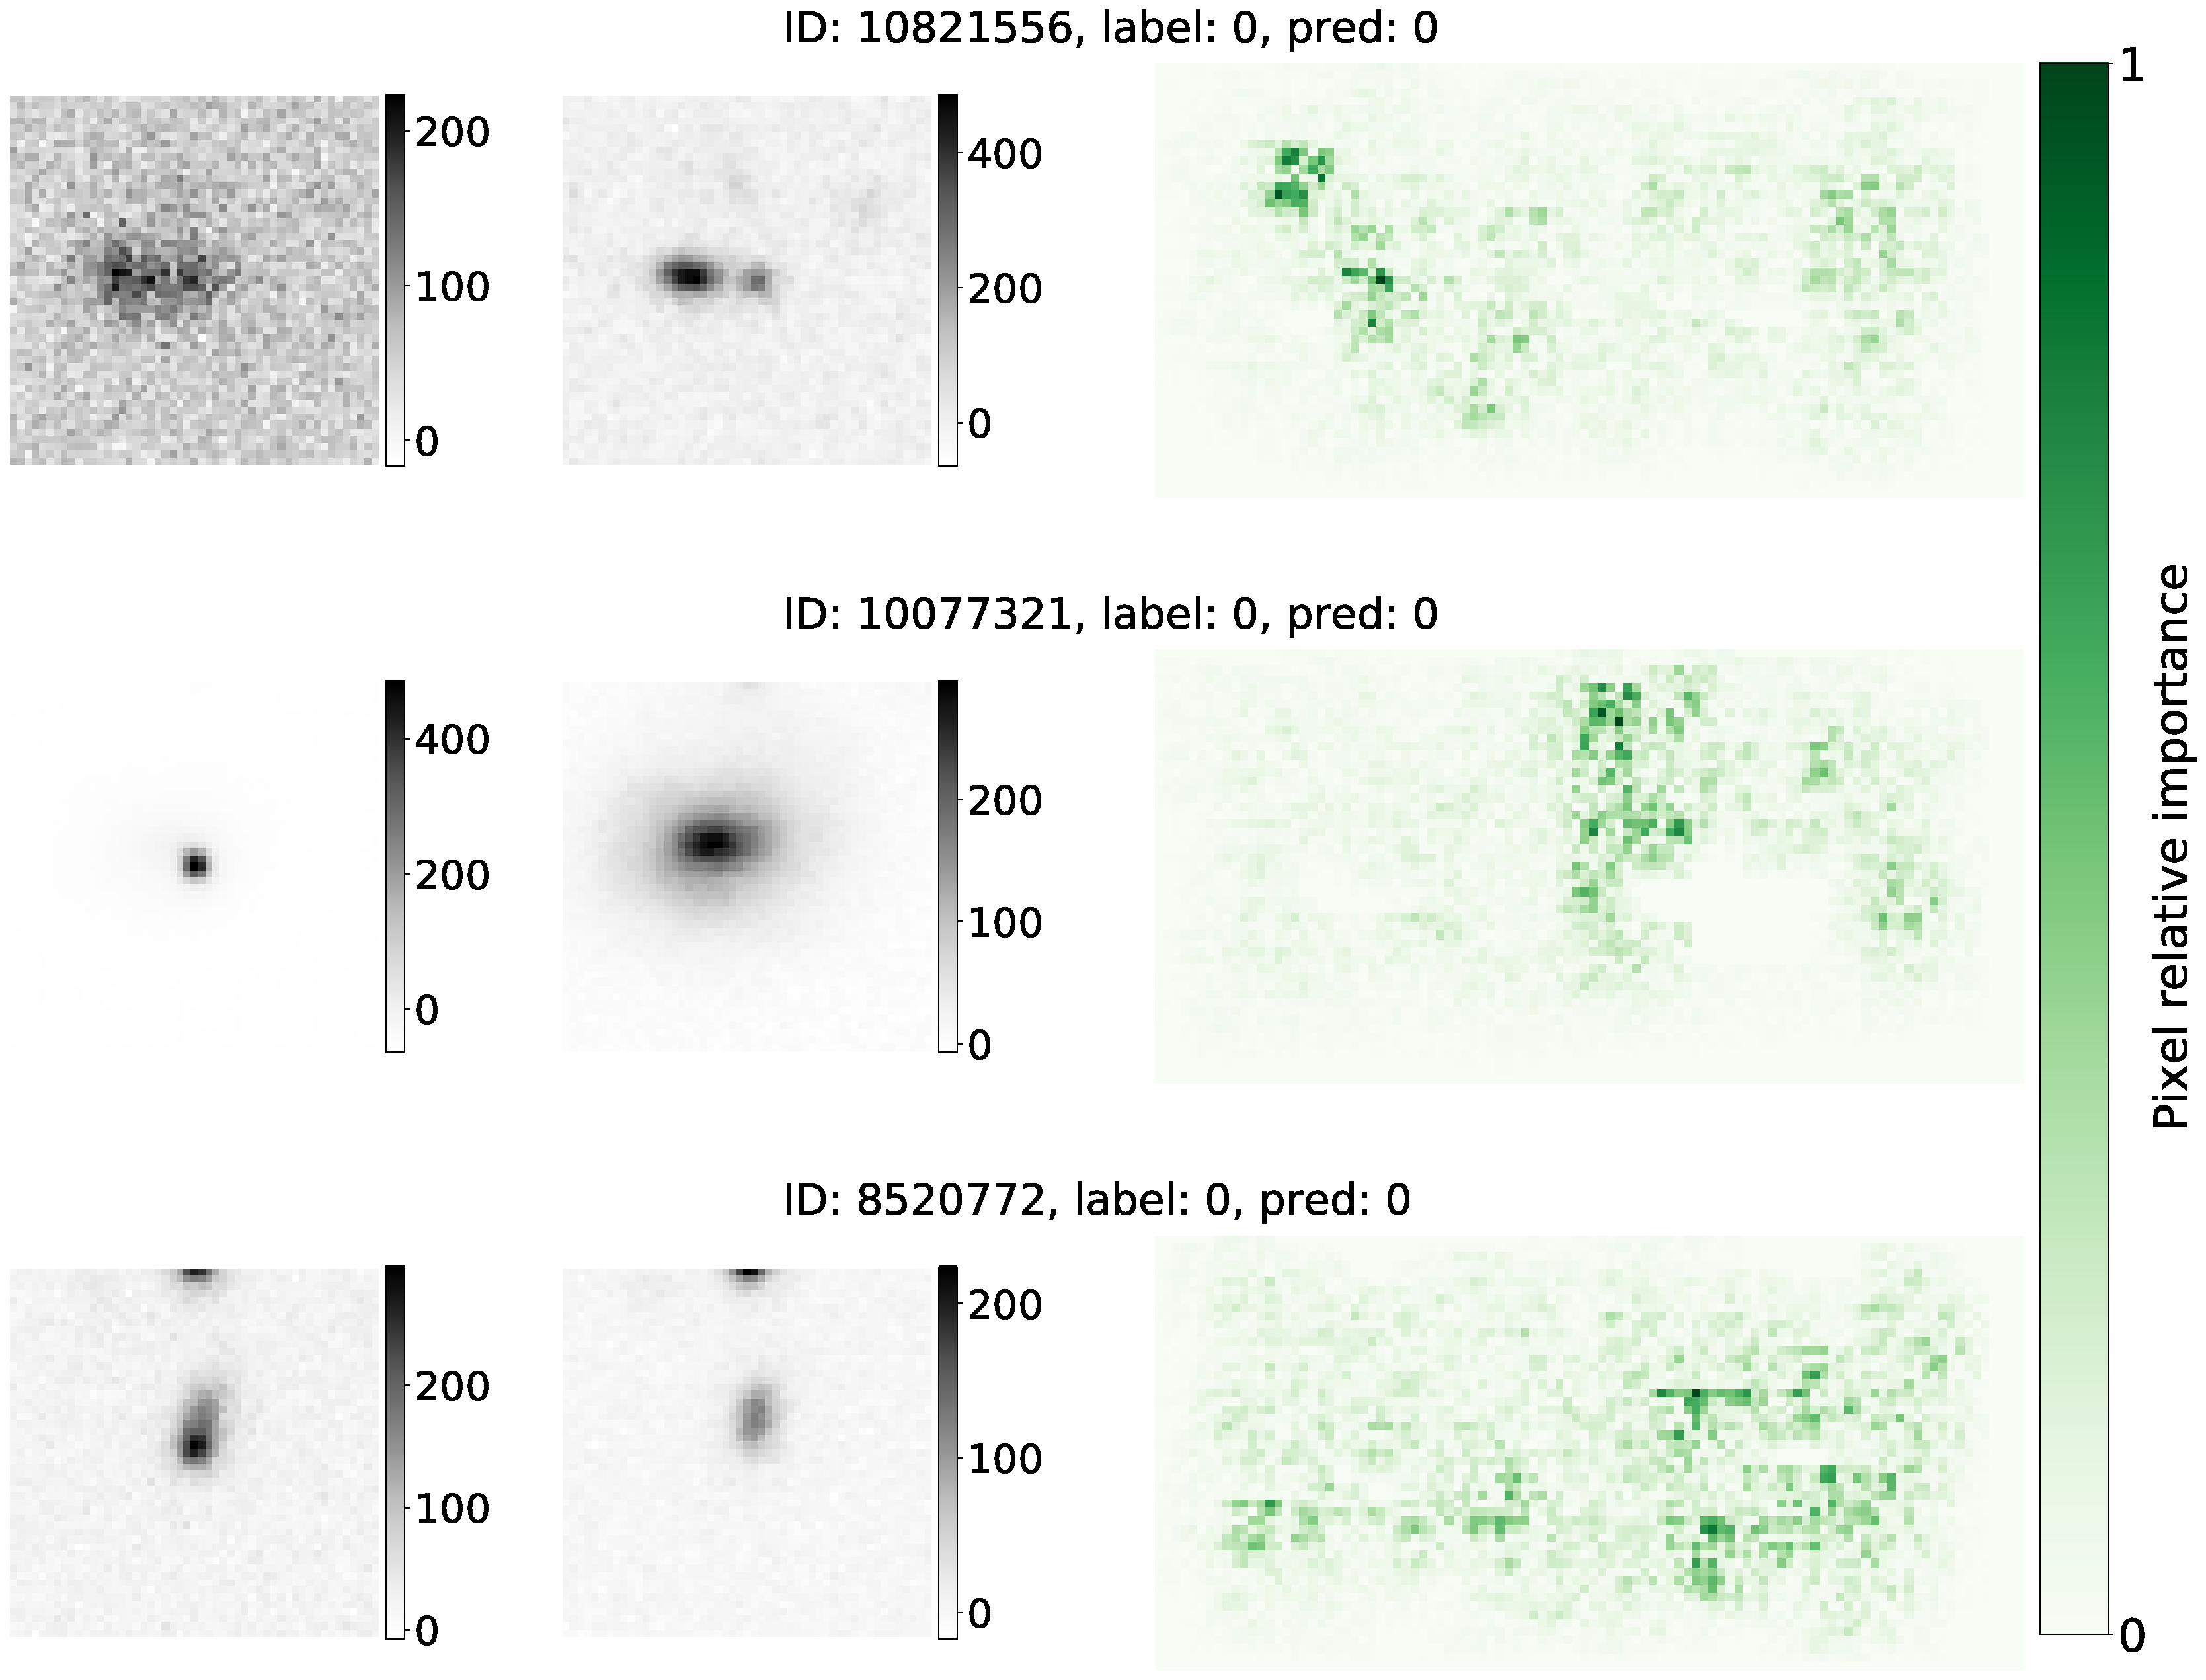
\includegraphics[width=0.8\linewidth]{
    figures/saliency_plot_other3nodiaTP-see7407.pdf}
   \caption{Transients (\search-\temp) and their respective saliency map for the \nodia\ model True Positives  (correctly identified ``real'' astrophysical transients). Important pixels are found everywhere in the image, as the CNN learns how to compare the \diff\ and \temp\ taking a synoptic look at the properties of each image component.}
    \label{fig:tpndia}
\end{figure*}

\begin{figure*}
    \centering
    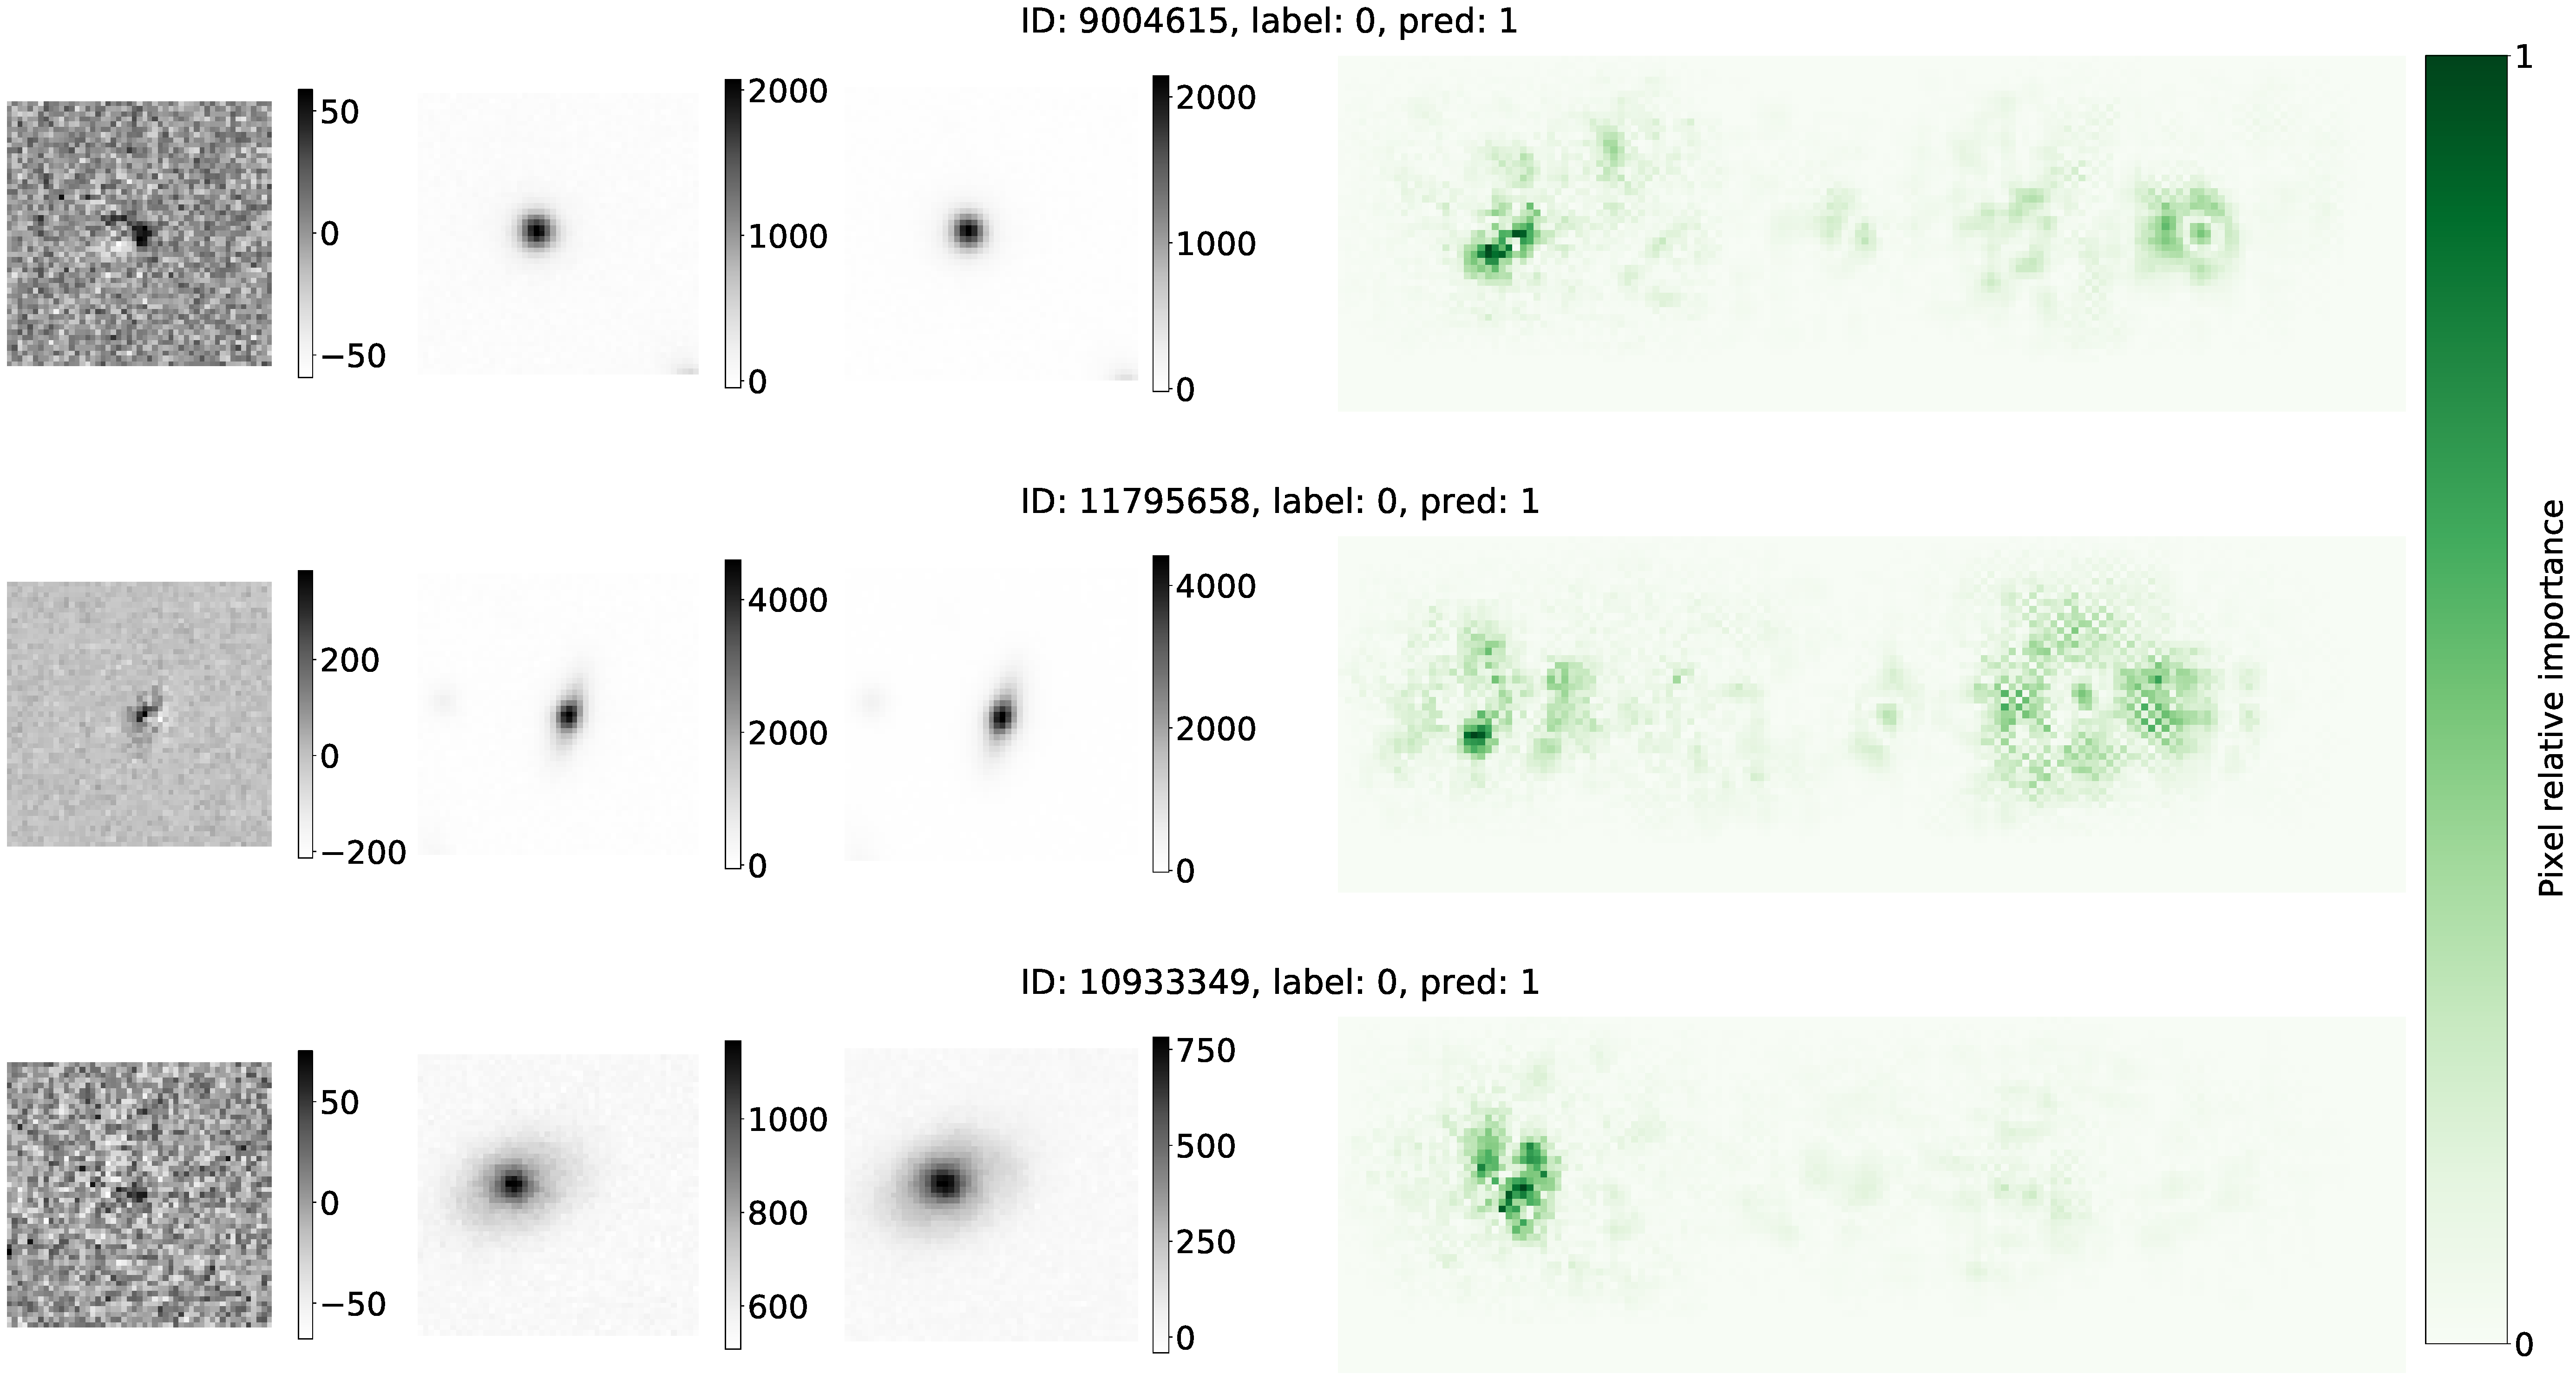
\includegraphics[width=0.8\linewidth]{
    figures/saliency_plot_other3FN-see66.pdf}
    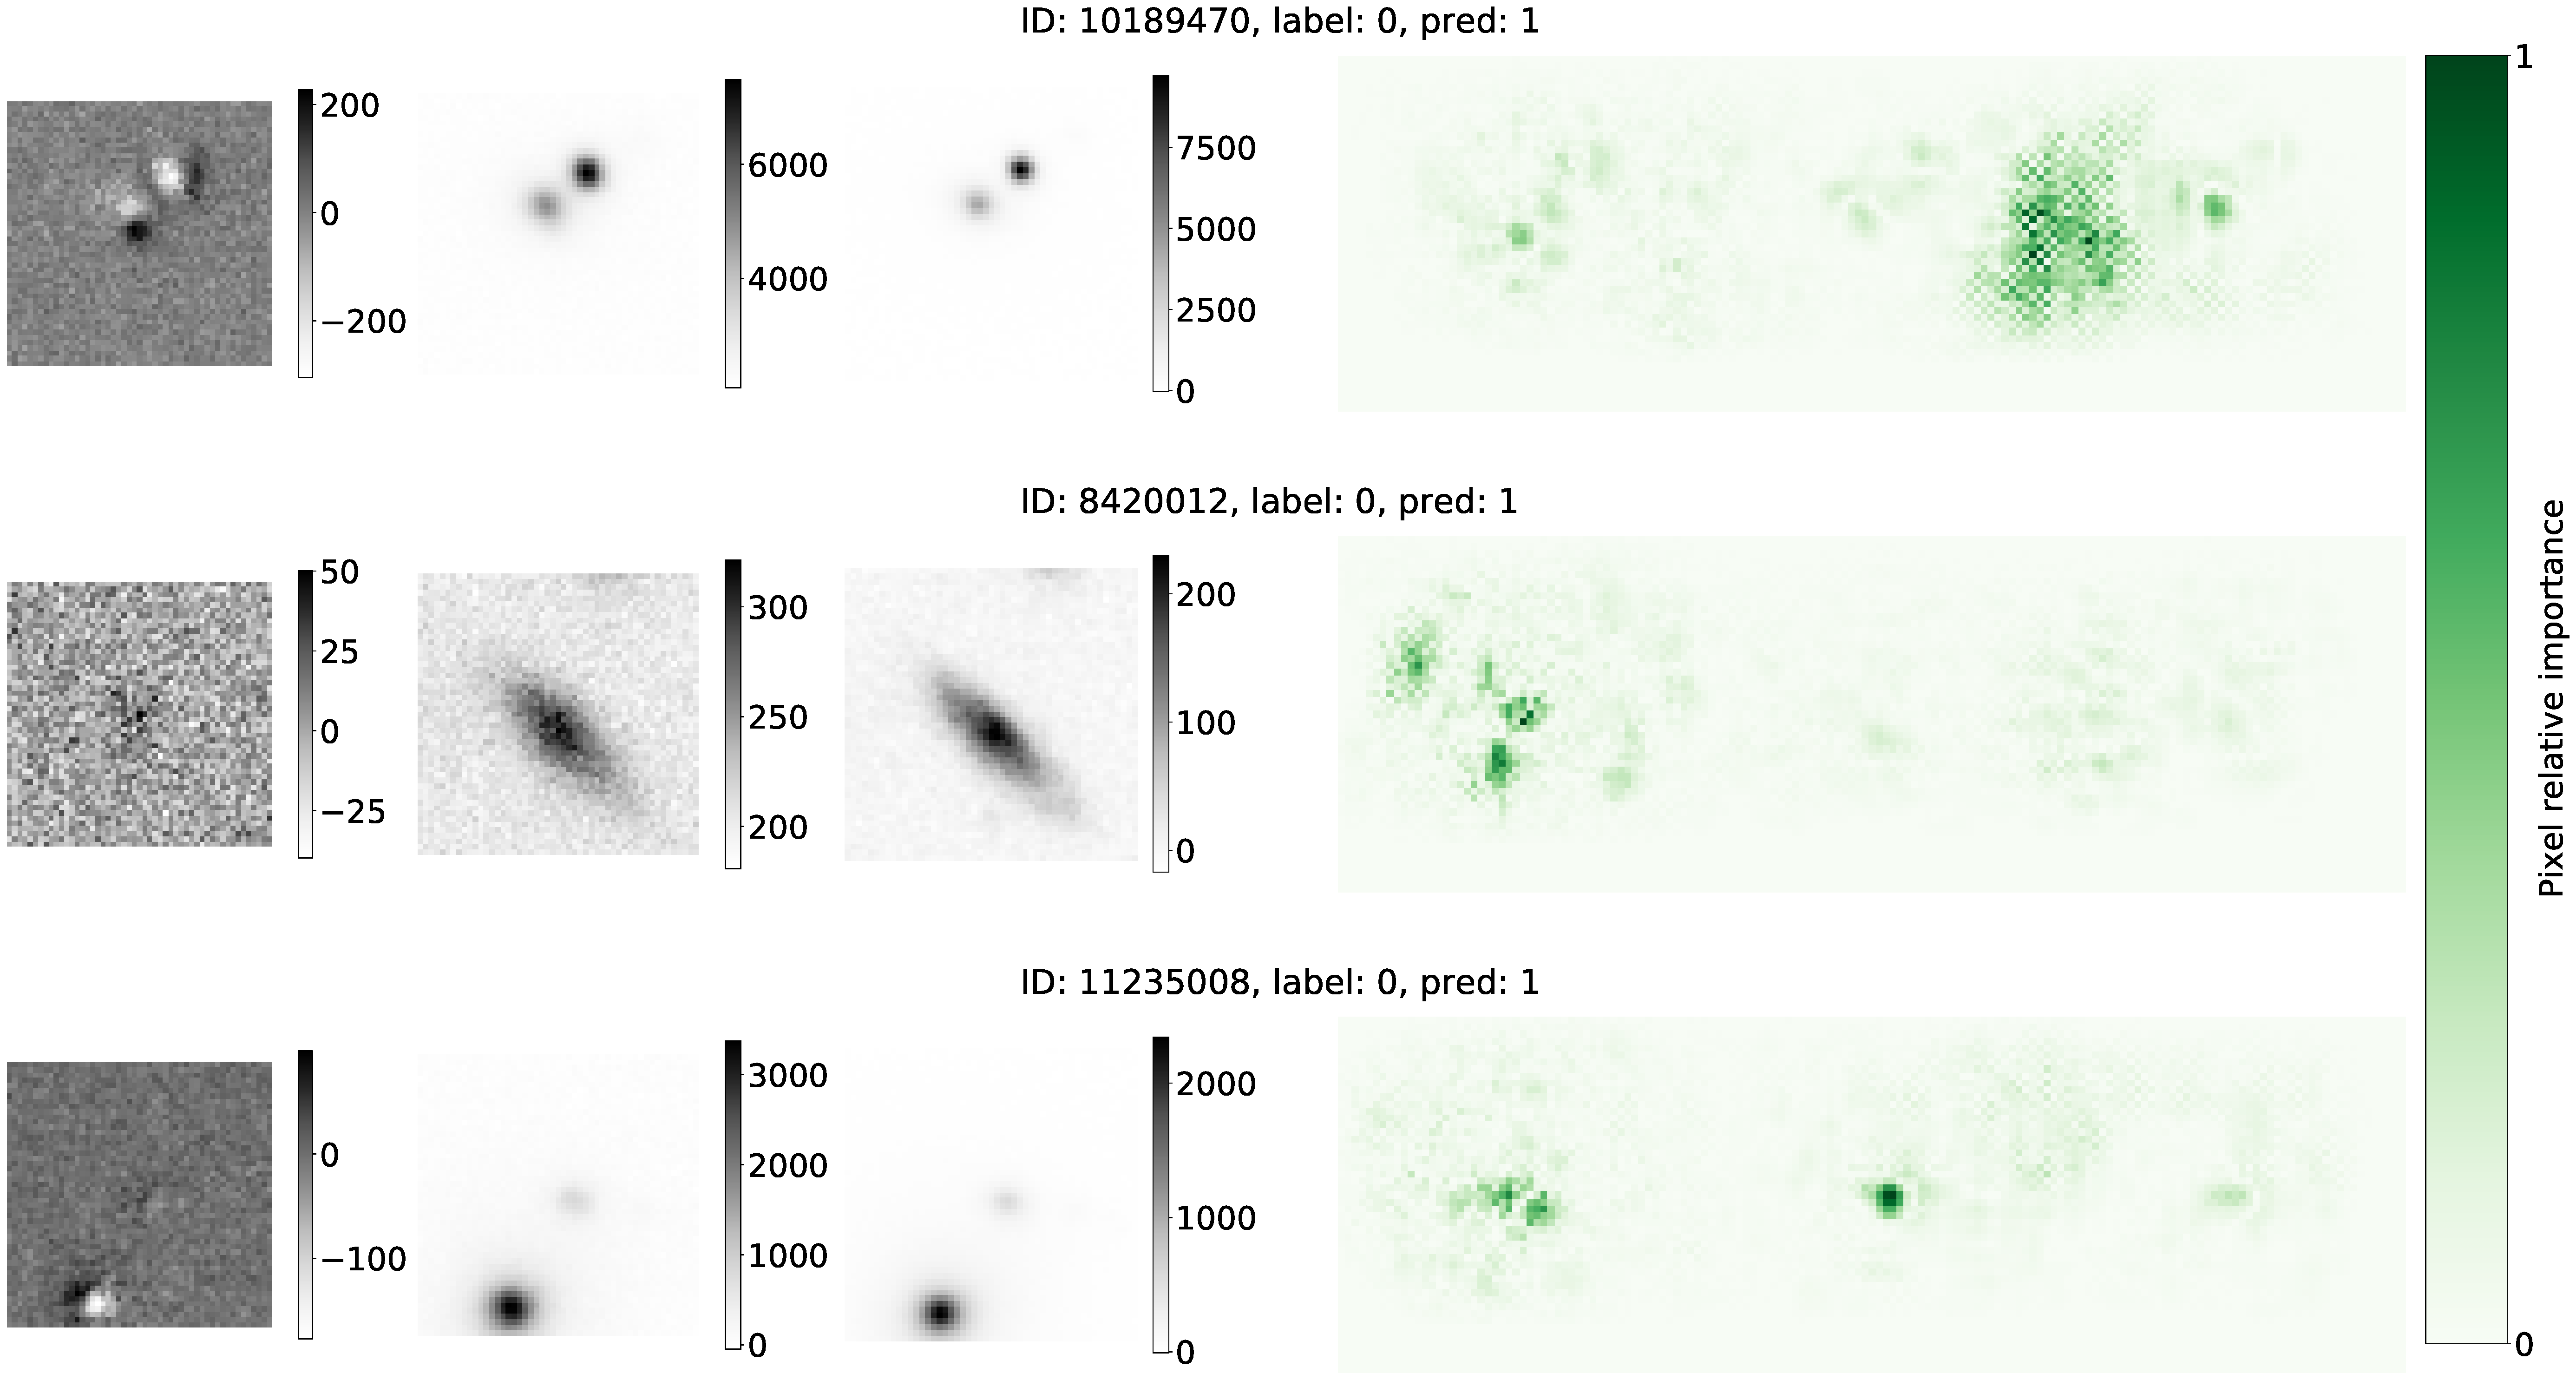
\includegraphics[width=0.8\linewidth]{
    figures/saliency_plot_other3FN-see2041.pdf}
    \caption{Transients (\diff-\search-\temp)  and their respective saliency map for \diabased\ model False Negatives (real transients identified as ``bogus'').
    We remind the reader that the labels are inherited from  \citet{Goldstein_2015} and cannot be verified. Some level of label inaccuracy is expected. The ``real'' transients in this dataset are implanted supernovae onto real DES images. However, in this collection, several transient display DIA inaccuracies (row 1, 2, 4, 6 show ``dipoles'', see \autoref{sec:DI}) that likely lead to the incorrect classification. Two very low signal-to-noise detections are missed (row 3 and 5) by our model.
    Important pixels are more commonly found in \diff\ portion of the image. In the \search\ saliency maps we see again that the core of the central source is used in the classification, as well as pixels that surround the source, but these two sets of important pixels are separate by it by a gap, again reminiscent of the typical aperture photometry technique (top two panels). } 
    \label{fig:saliency_dia3id_FN}
\end{figure*}




\begin{figure*}
    \centering
    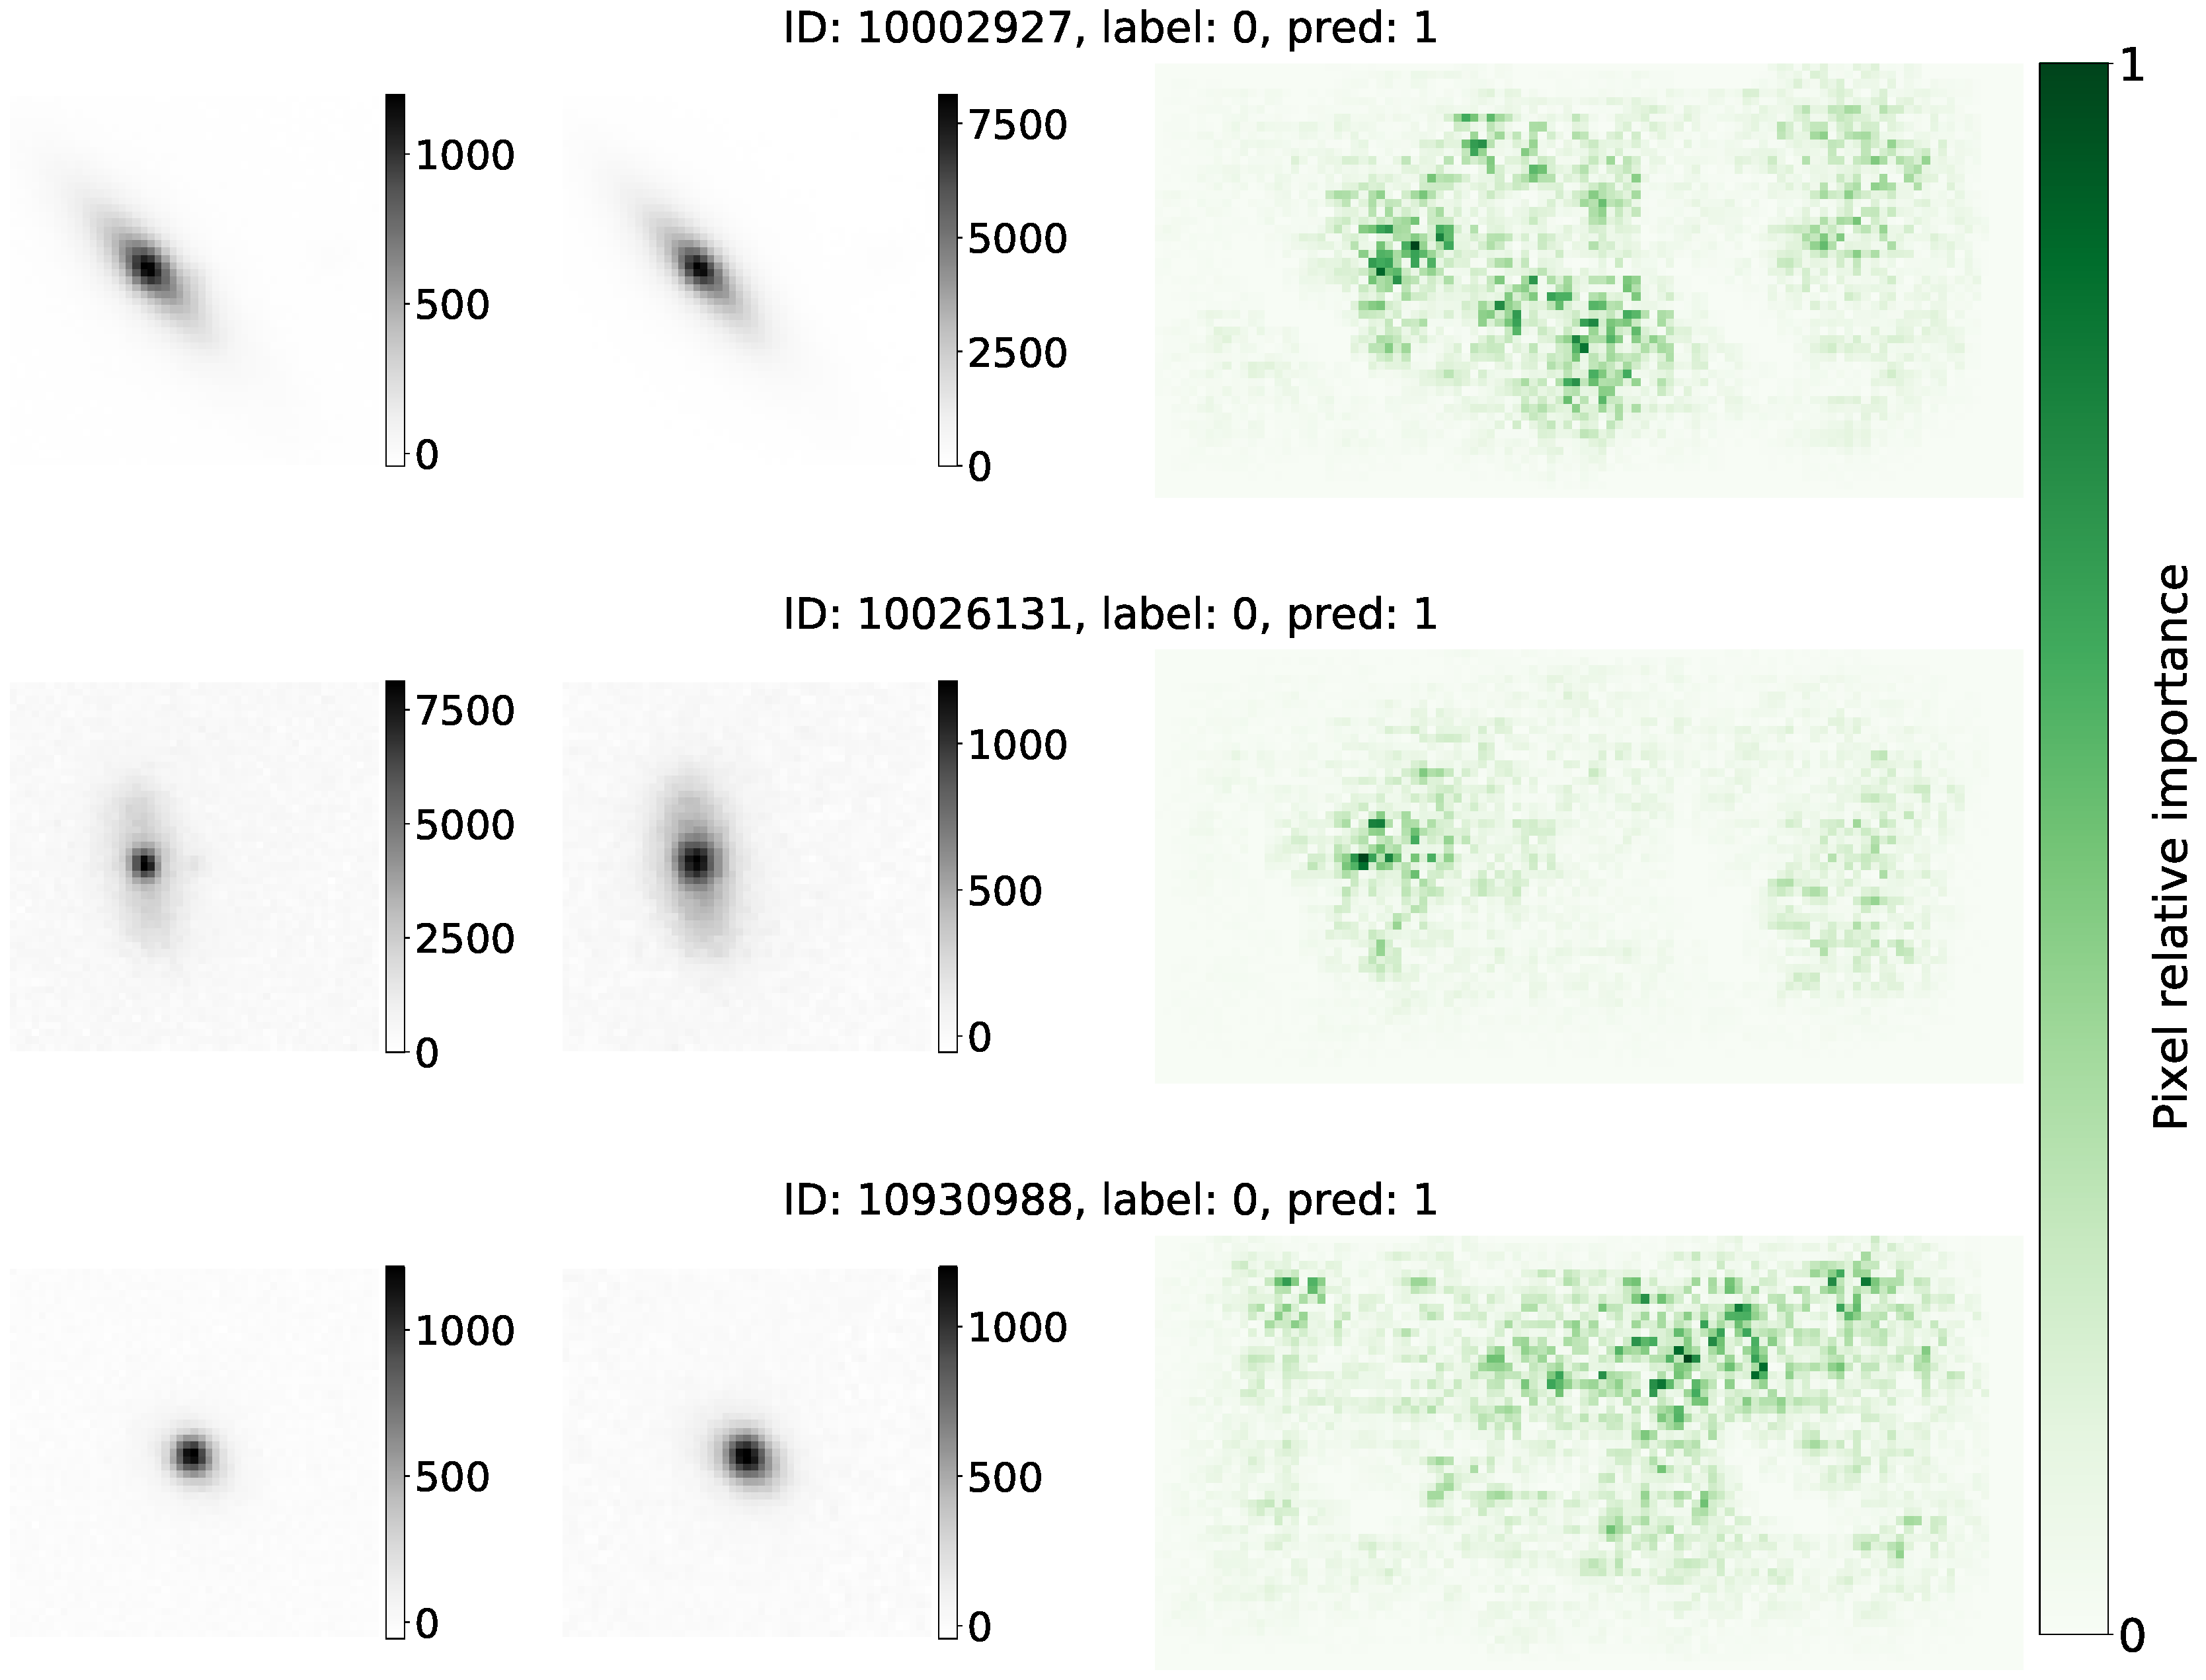
\includegraphics[width=0.76\linewidth]{
    figures/saliency_plot_other3nodiaFN-see356.pdf}
    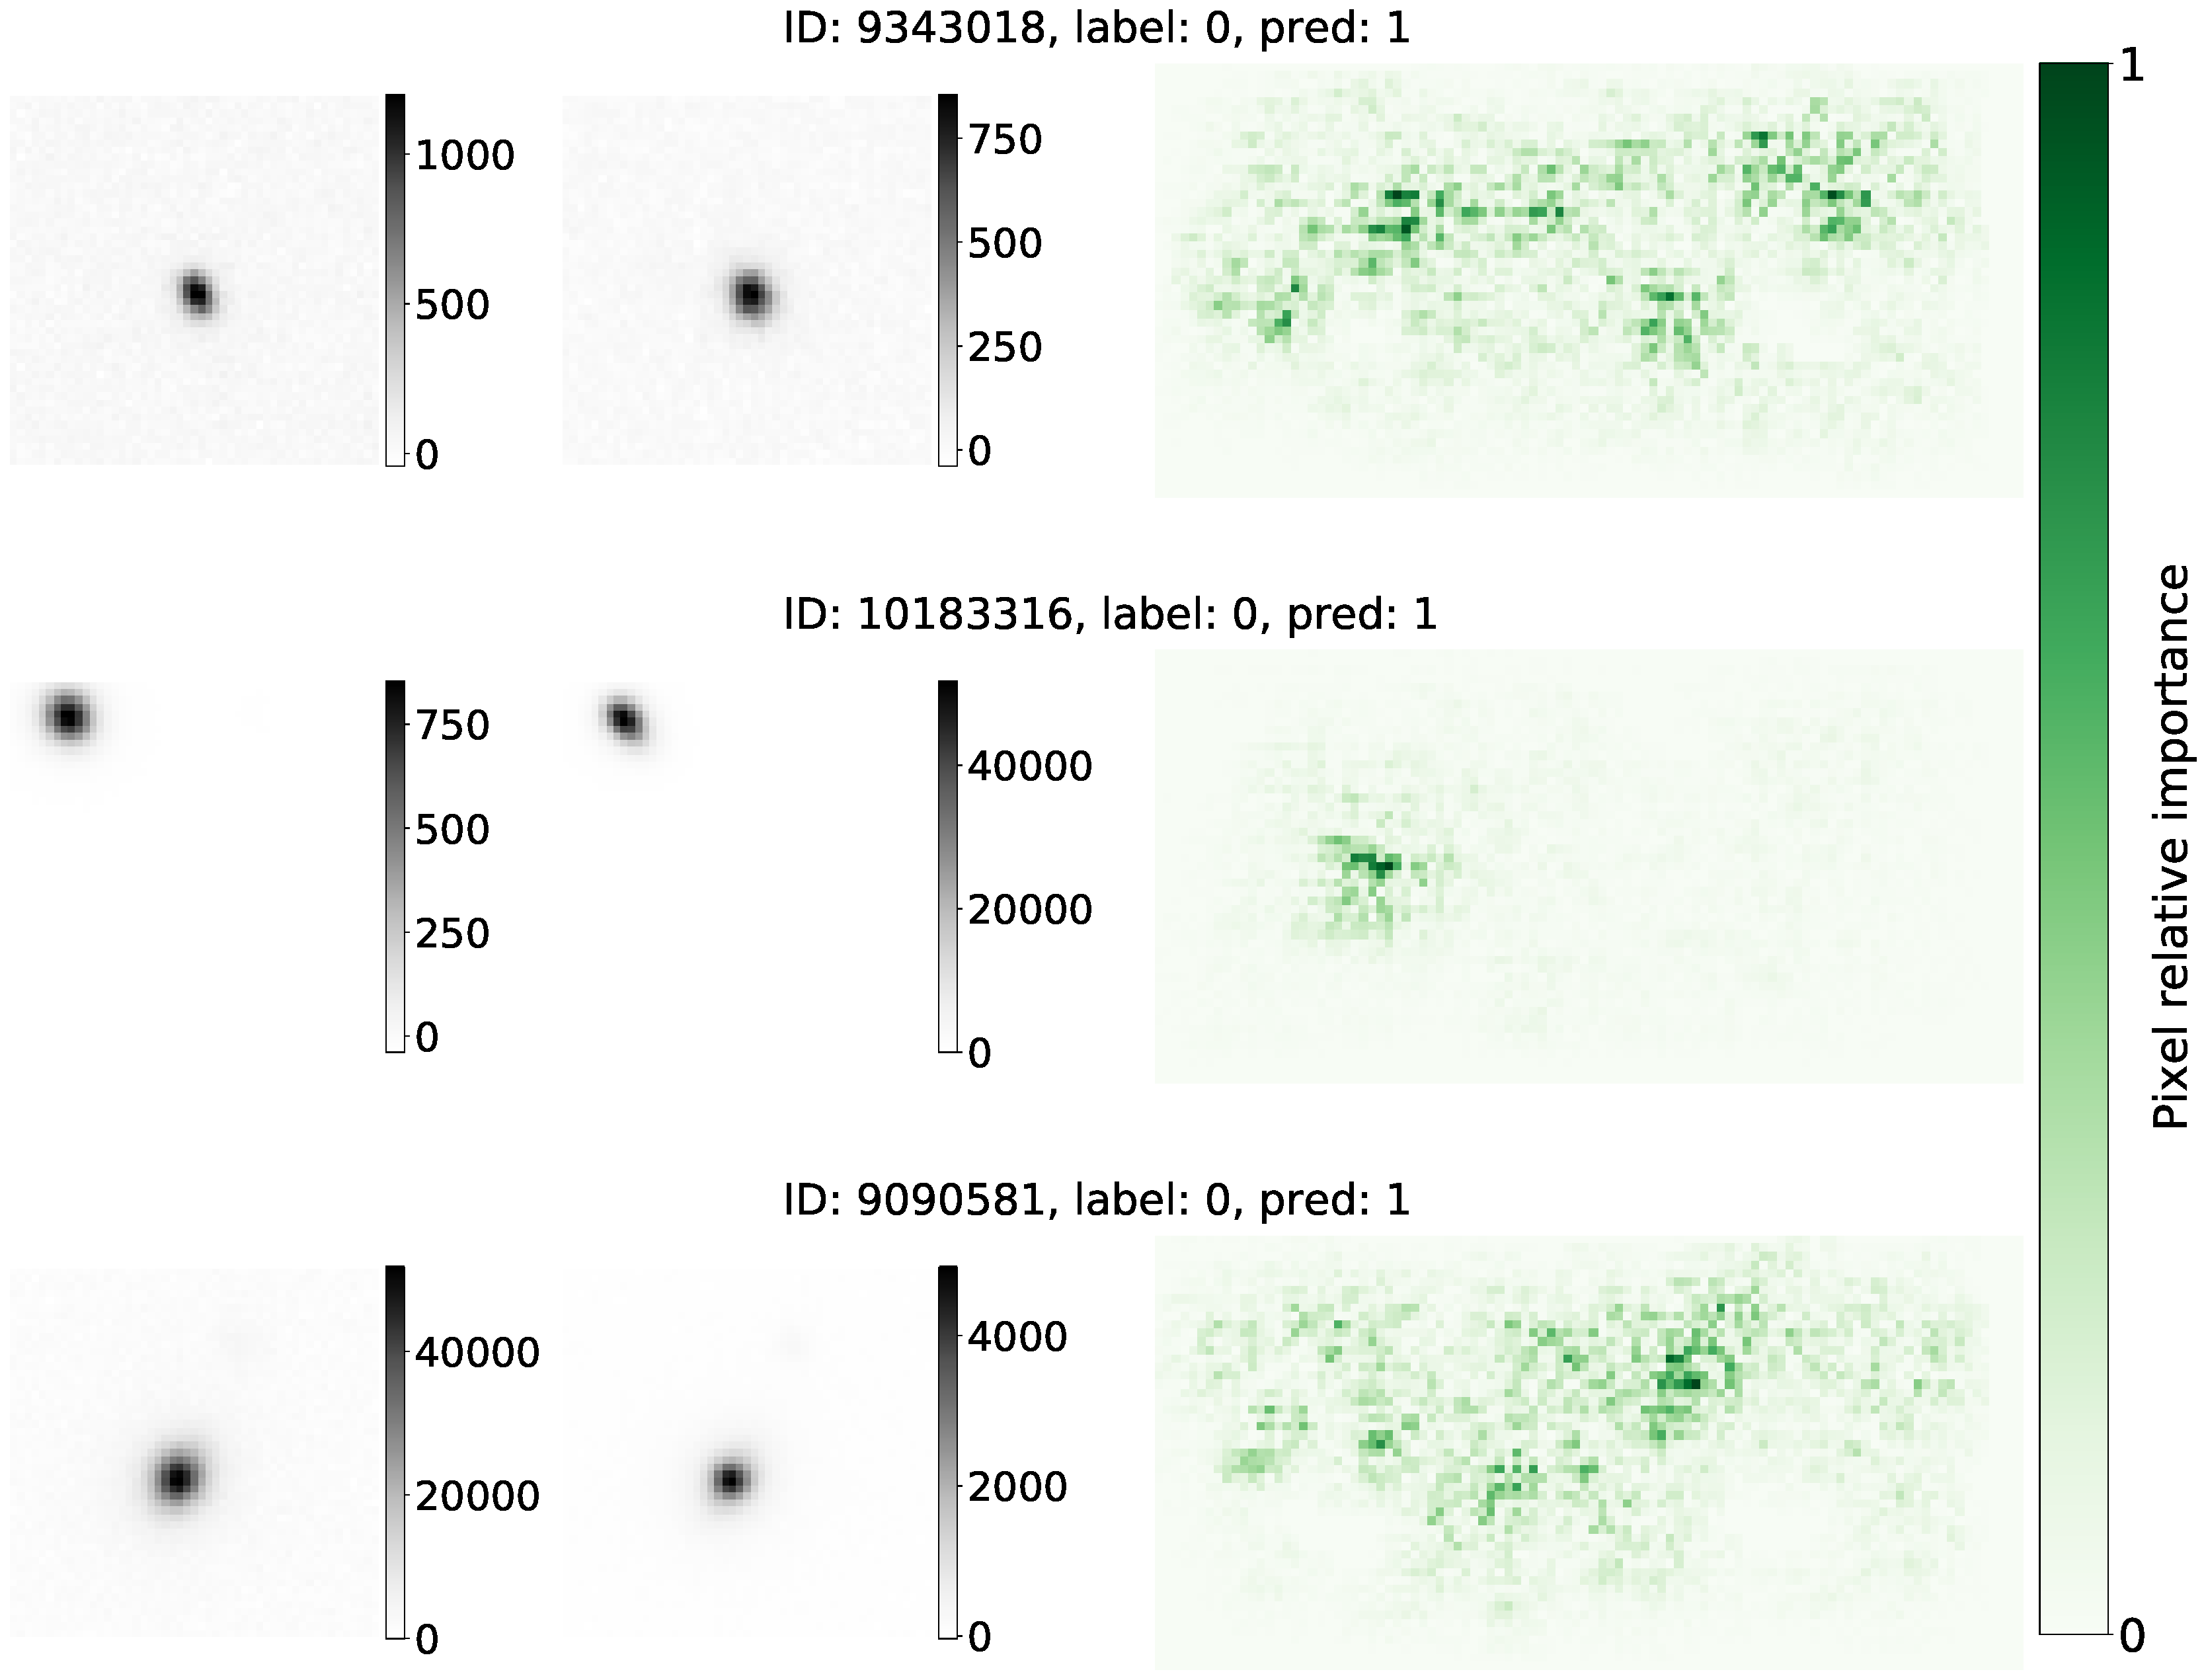
\includegraphics[width=0.76\linewidth]{
    figures/saliency_plot_other3nodiaFN-see981.pdf}
    \caption{
    Transients (\search-\temp) and their respective saliency map for the \nodia\ model False Negatives (astrophysical sources classified as ``bogus''). In all cases but row 5 it is not clear why the classification fails. In row 5, another source dominates the image scaling (and pre-processing) reducing the visibility of the transient (that is completely missed by human inspection). We remind the reader that the ``real'' transients in this dataset are implanted supernovae onto real DES images. Important pixels are found everywhere in the image, as the CNN learns how to compare the \diff\ and \temp\ taking a synoptic look at the properties of each image component.}
    \label{fig:fnndia}
\end{figure*}



\begin{figure*}
    \centering
    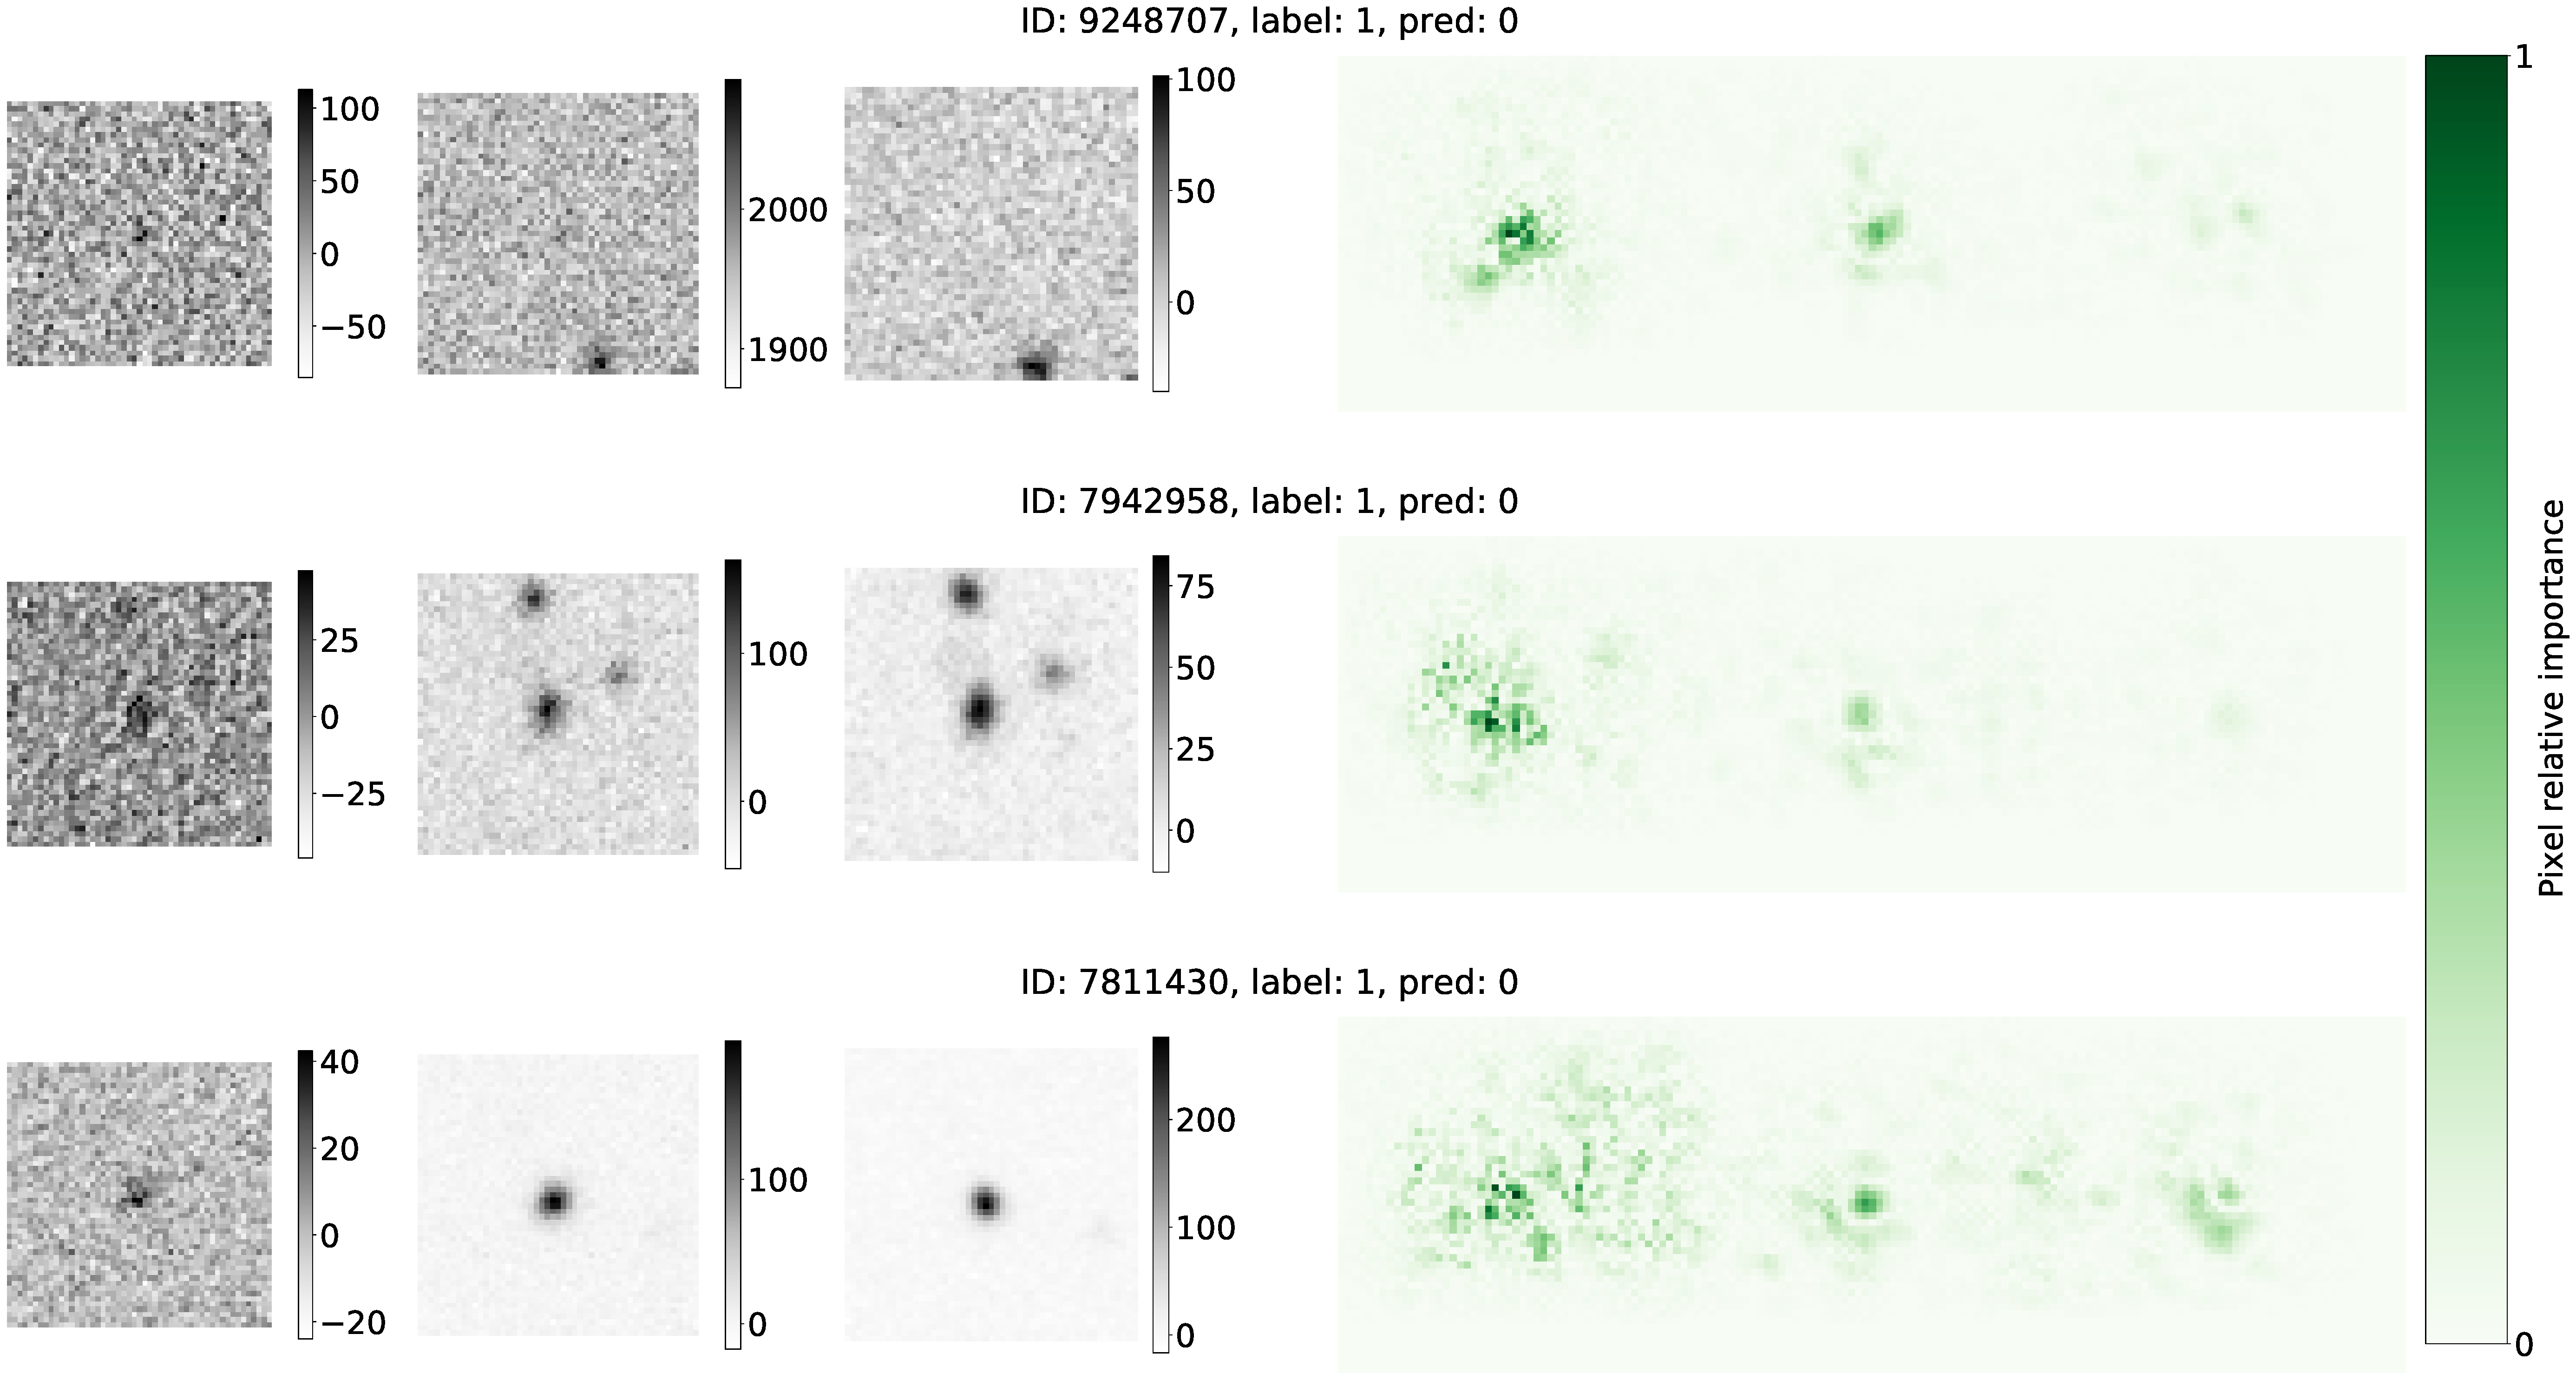
\includegraphics[width=0.8\linewidth]{
    figures/saliency_plot_other3FP-see21.pdf}
    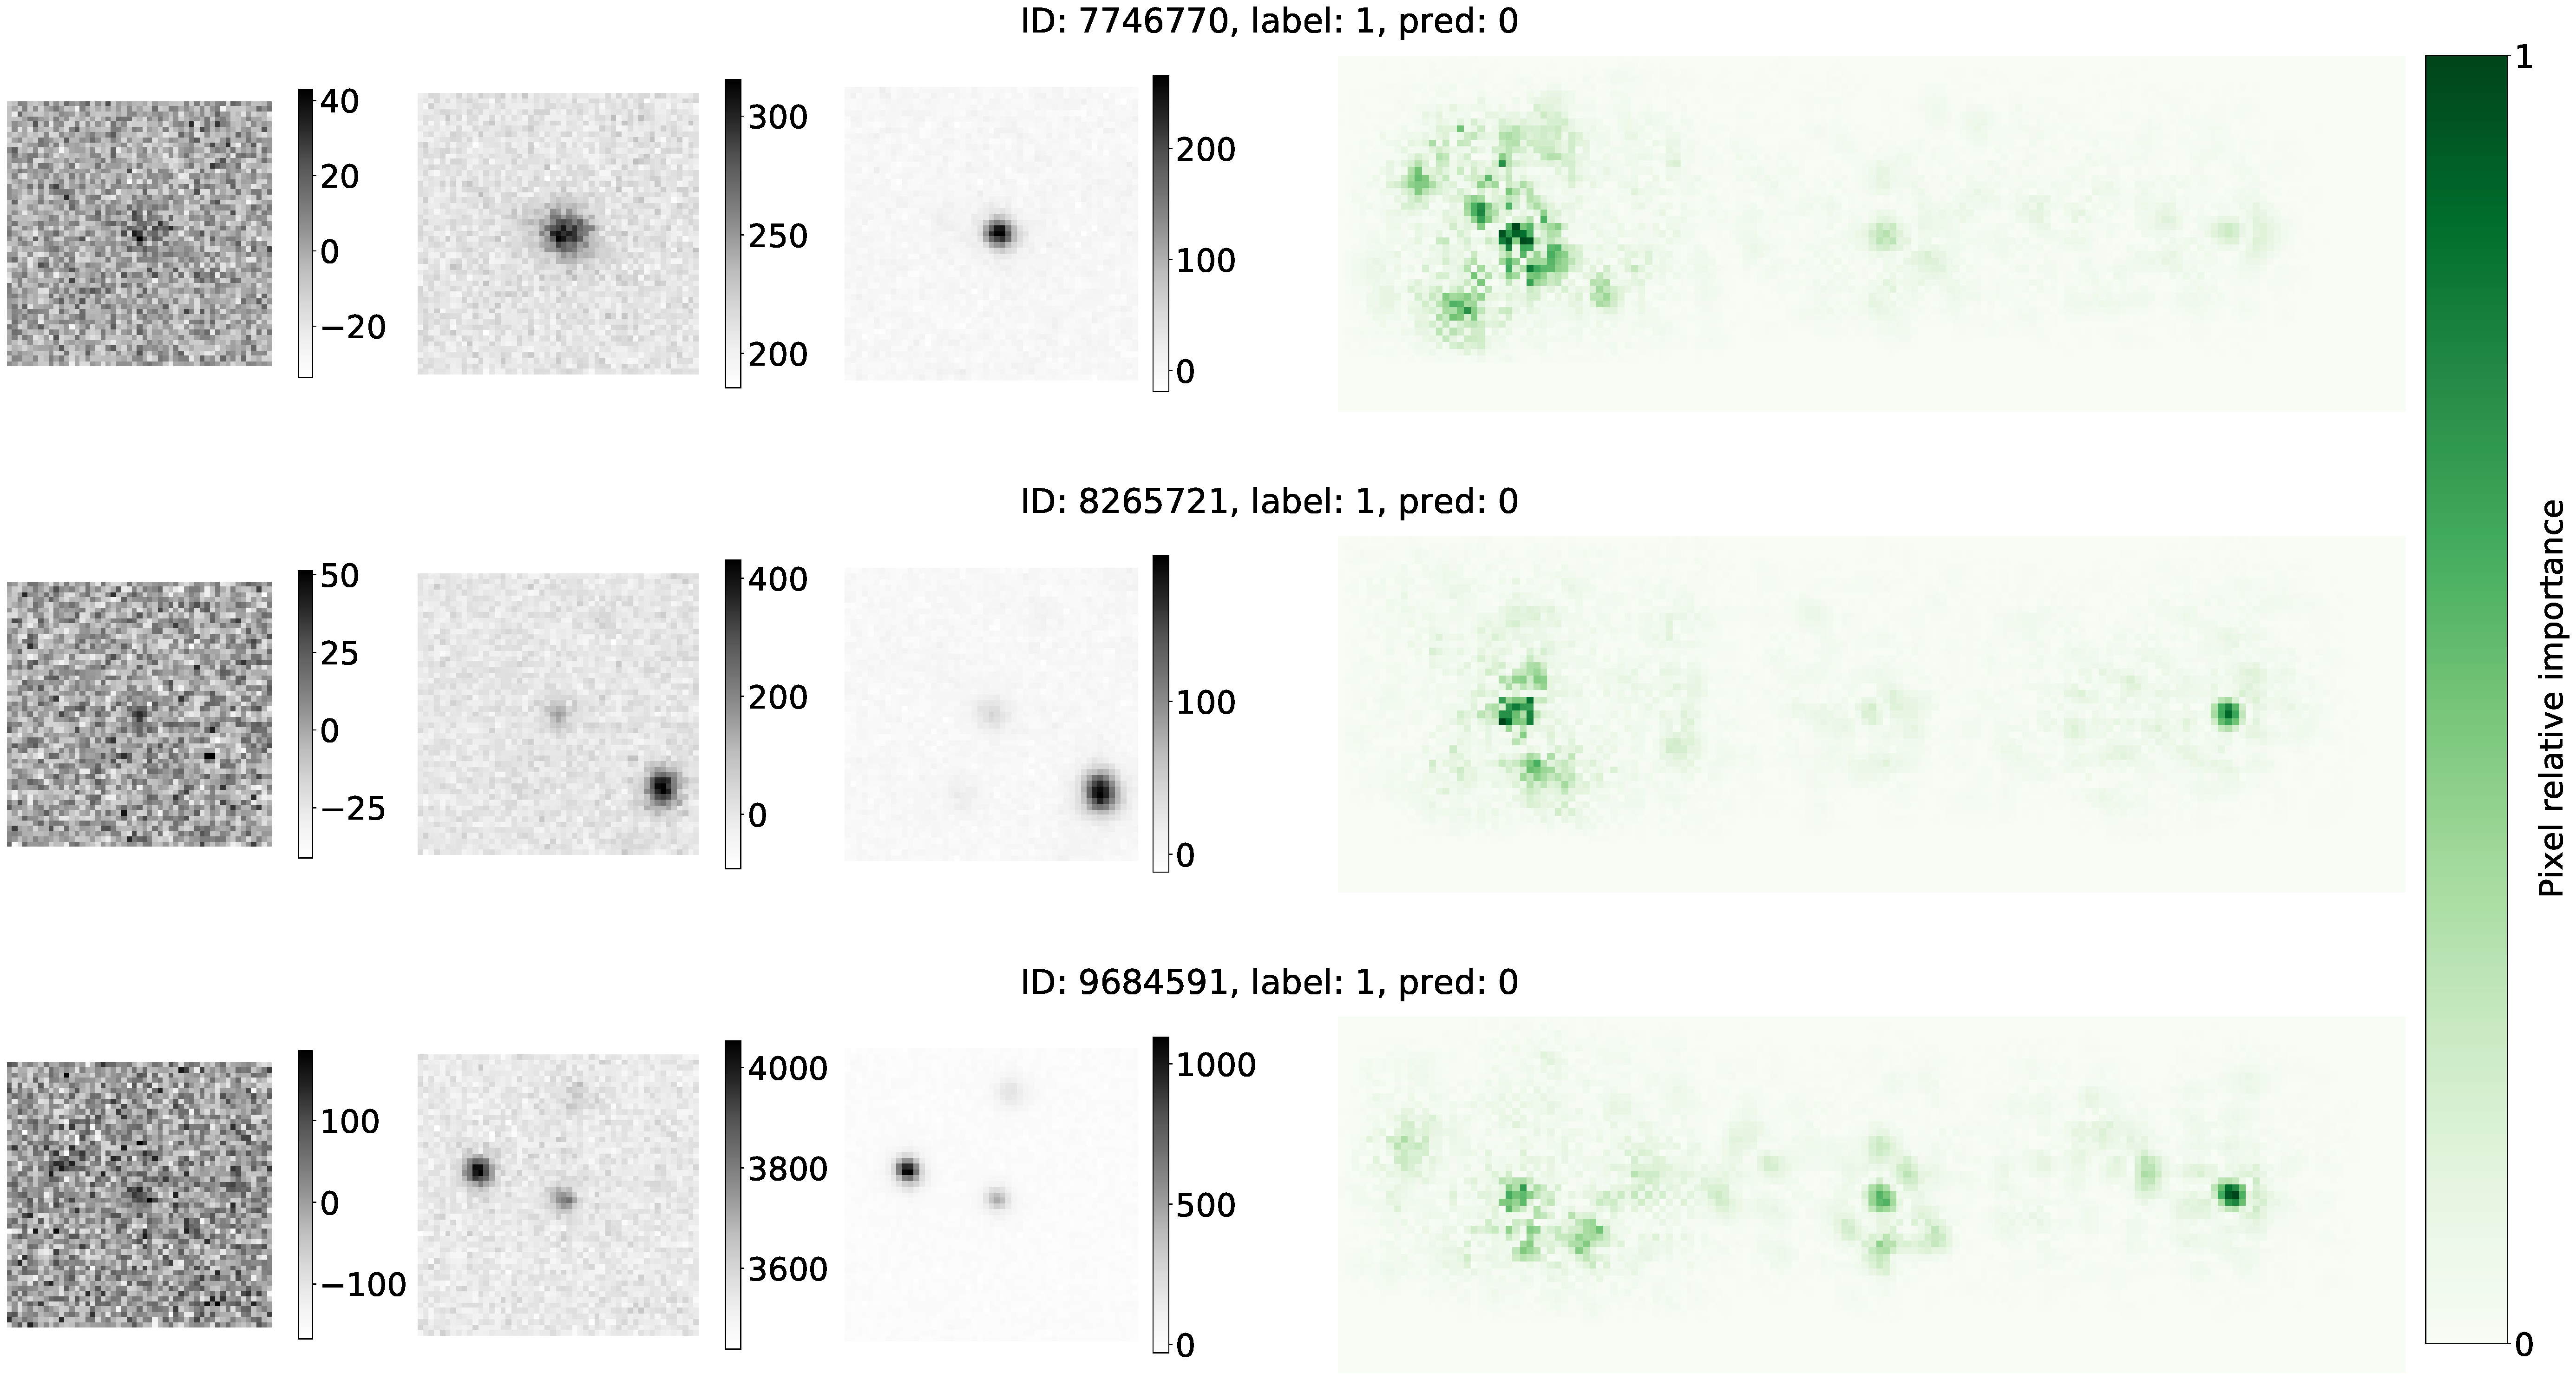
\includegraphics[width=0.8\linewidth]{
    figures/saliency_plot_other3FP-see369.pdf}
    \caption{Transients (\diff-\search-\temp) and their respective saliency map for \diabased\ model False Positives (``bogus'' predicted as ``real'').  We remind the reader again that the labels are inherited from  \citet{Goldstein_2015} and cannot be verified.  Some level of label inaccuracy is expected. Bogus transients were labeled by human scanners among astrophysical images with detection. However, in this collection, we cannot verify the nature of the transient and we argue that in the cases presented here there is no obvious evidence of its ``bogus'' nature. Important pixels are most commonly found in the \diff, but in \temp\ and \search\ we see again the CNN analyzes the central source and its surrounding, but avoiding the tail of the central source, in a way similar to traditional aperture photometry techniques.}
    \label{fig:saliency_dia3id_FP}
\end{figure*}
\begin{figure*}
    \centering
    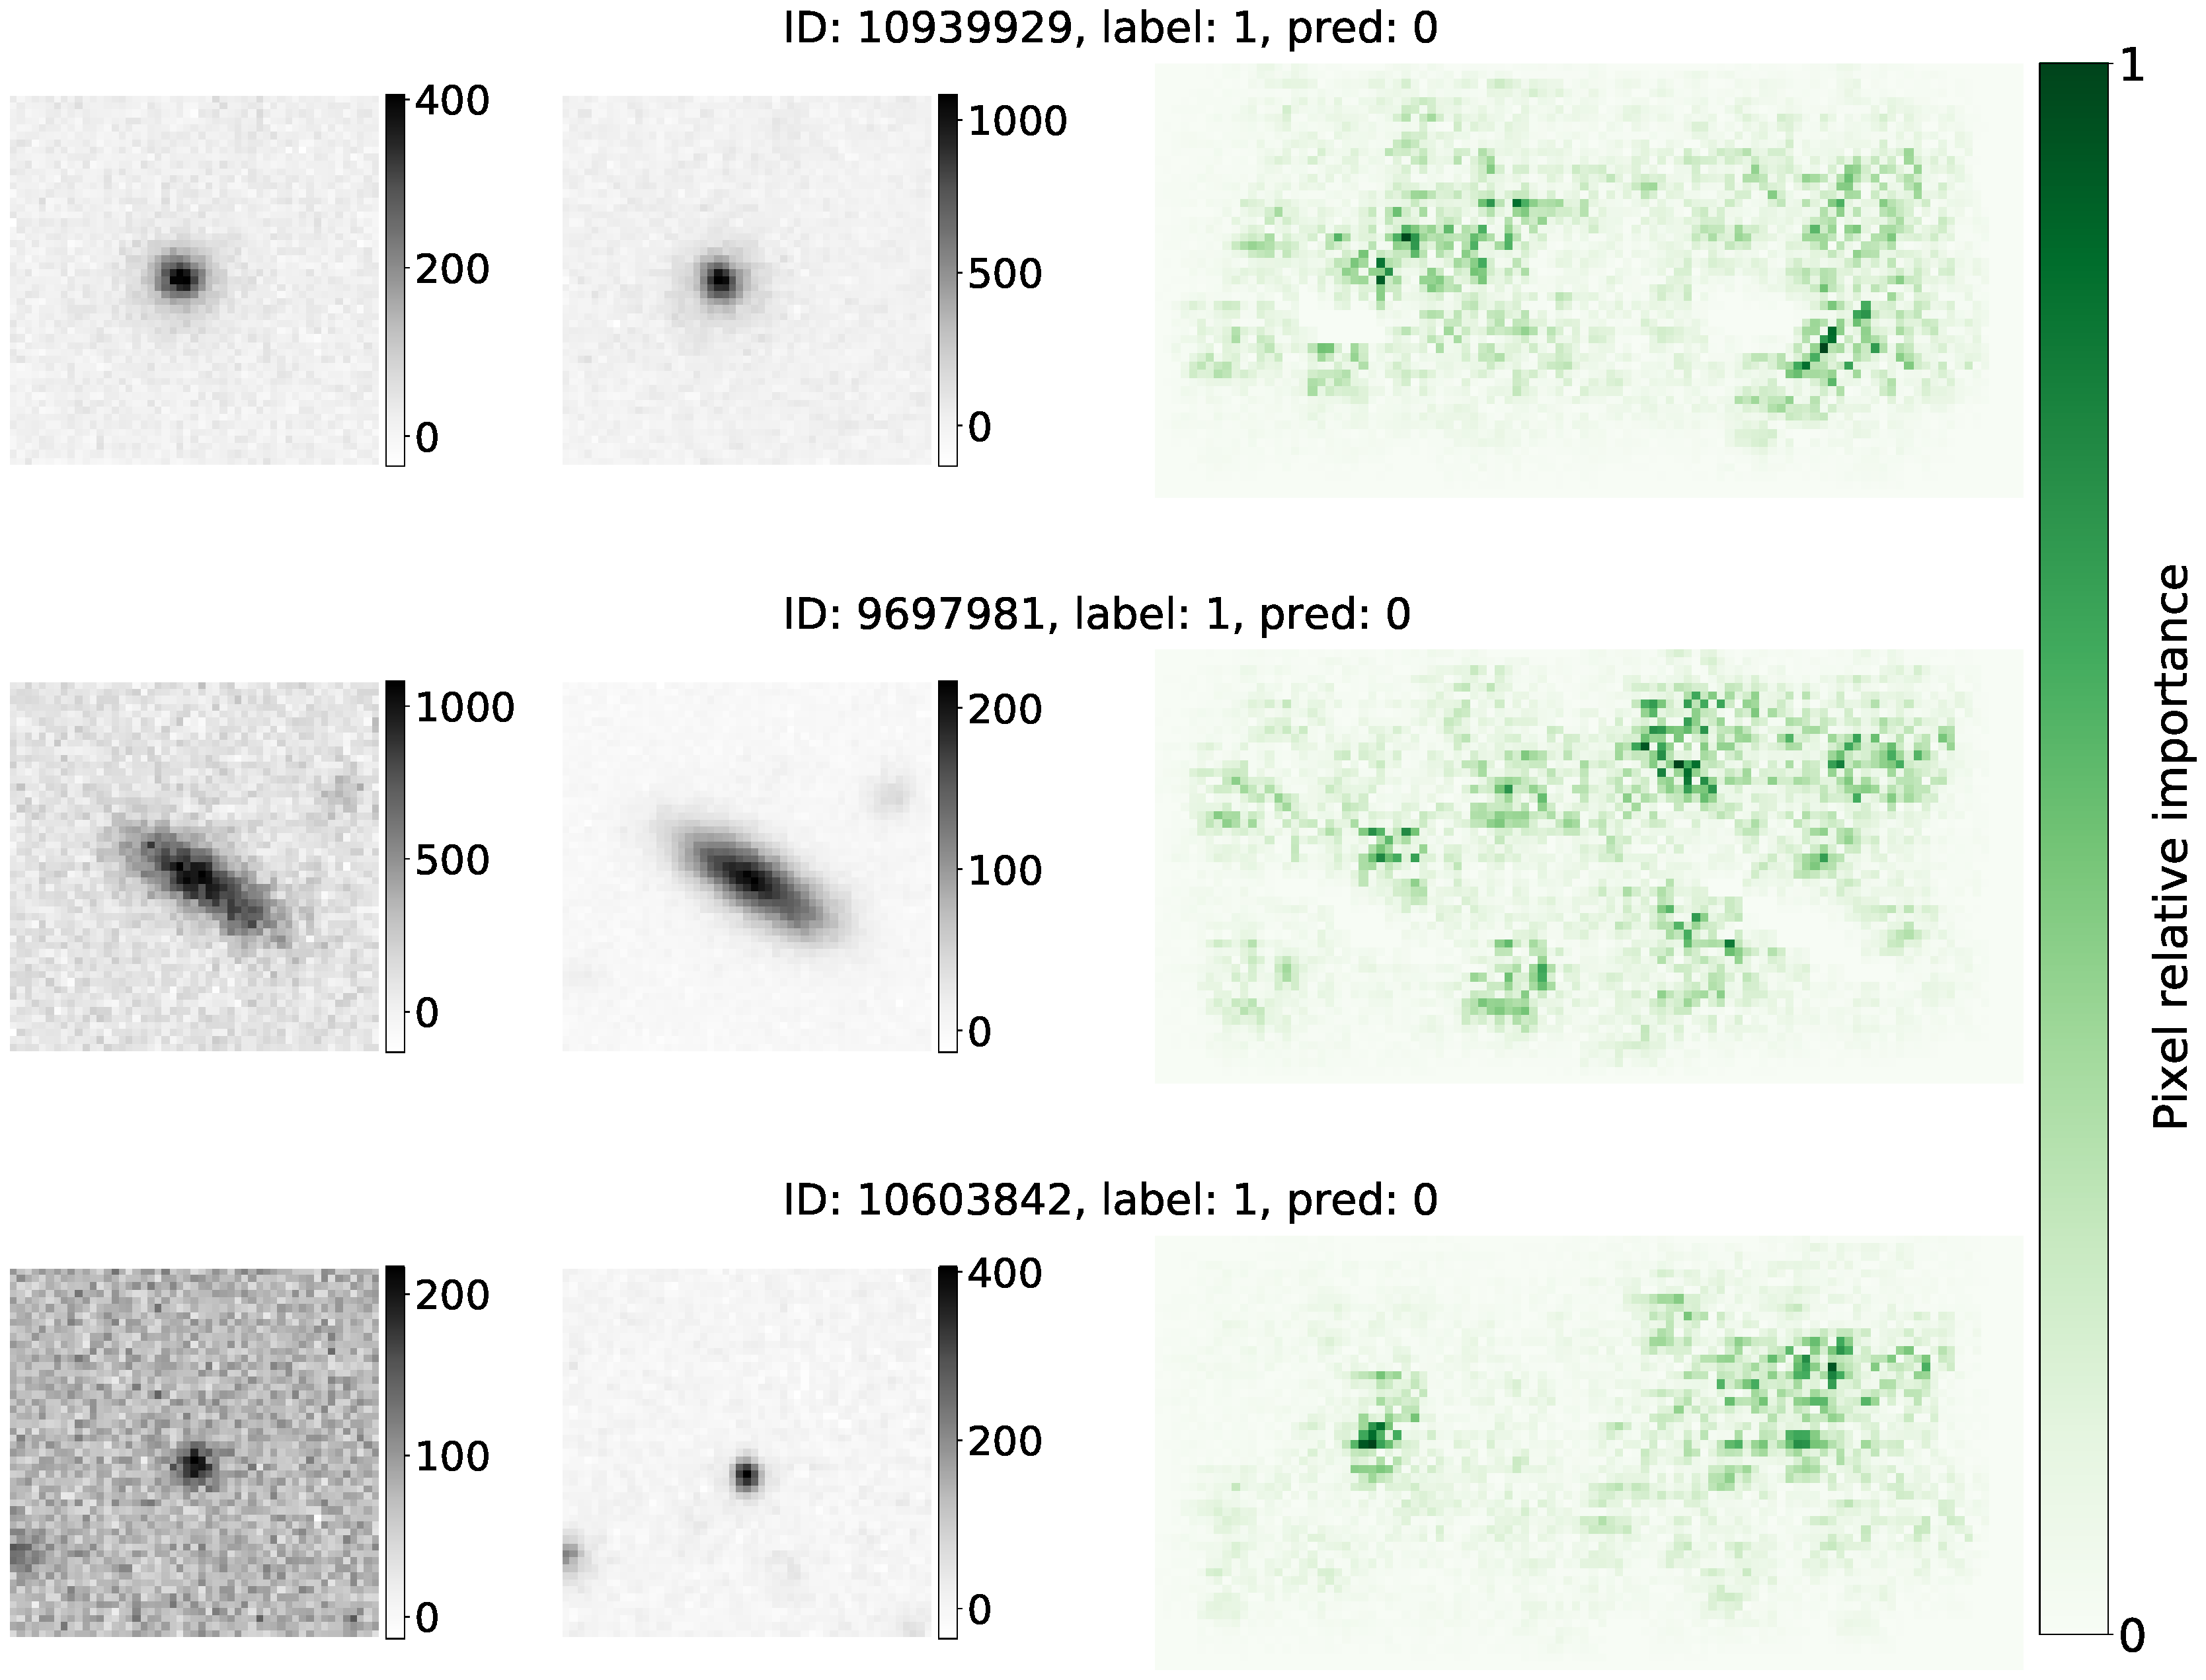
\includegraphics[width=0.76\linewidth]{
    figures/saliency_plot_other3nodiaFP-see18.pdf}
    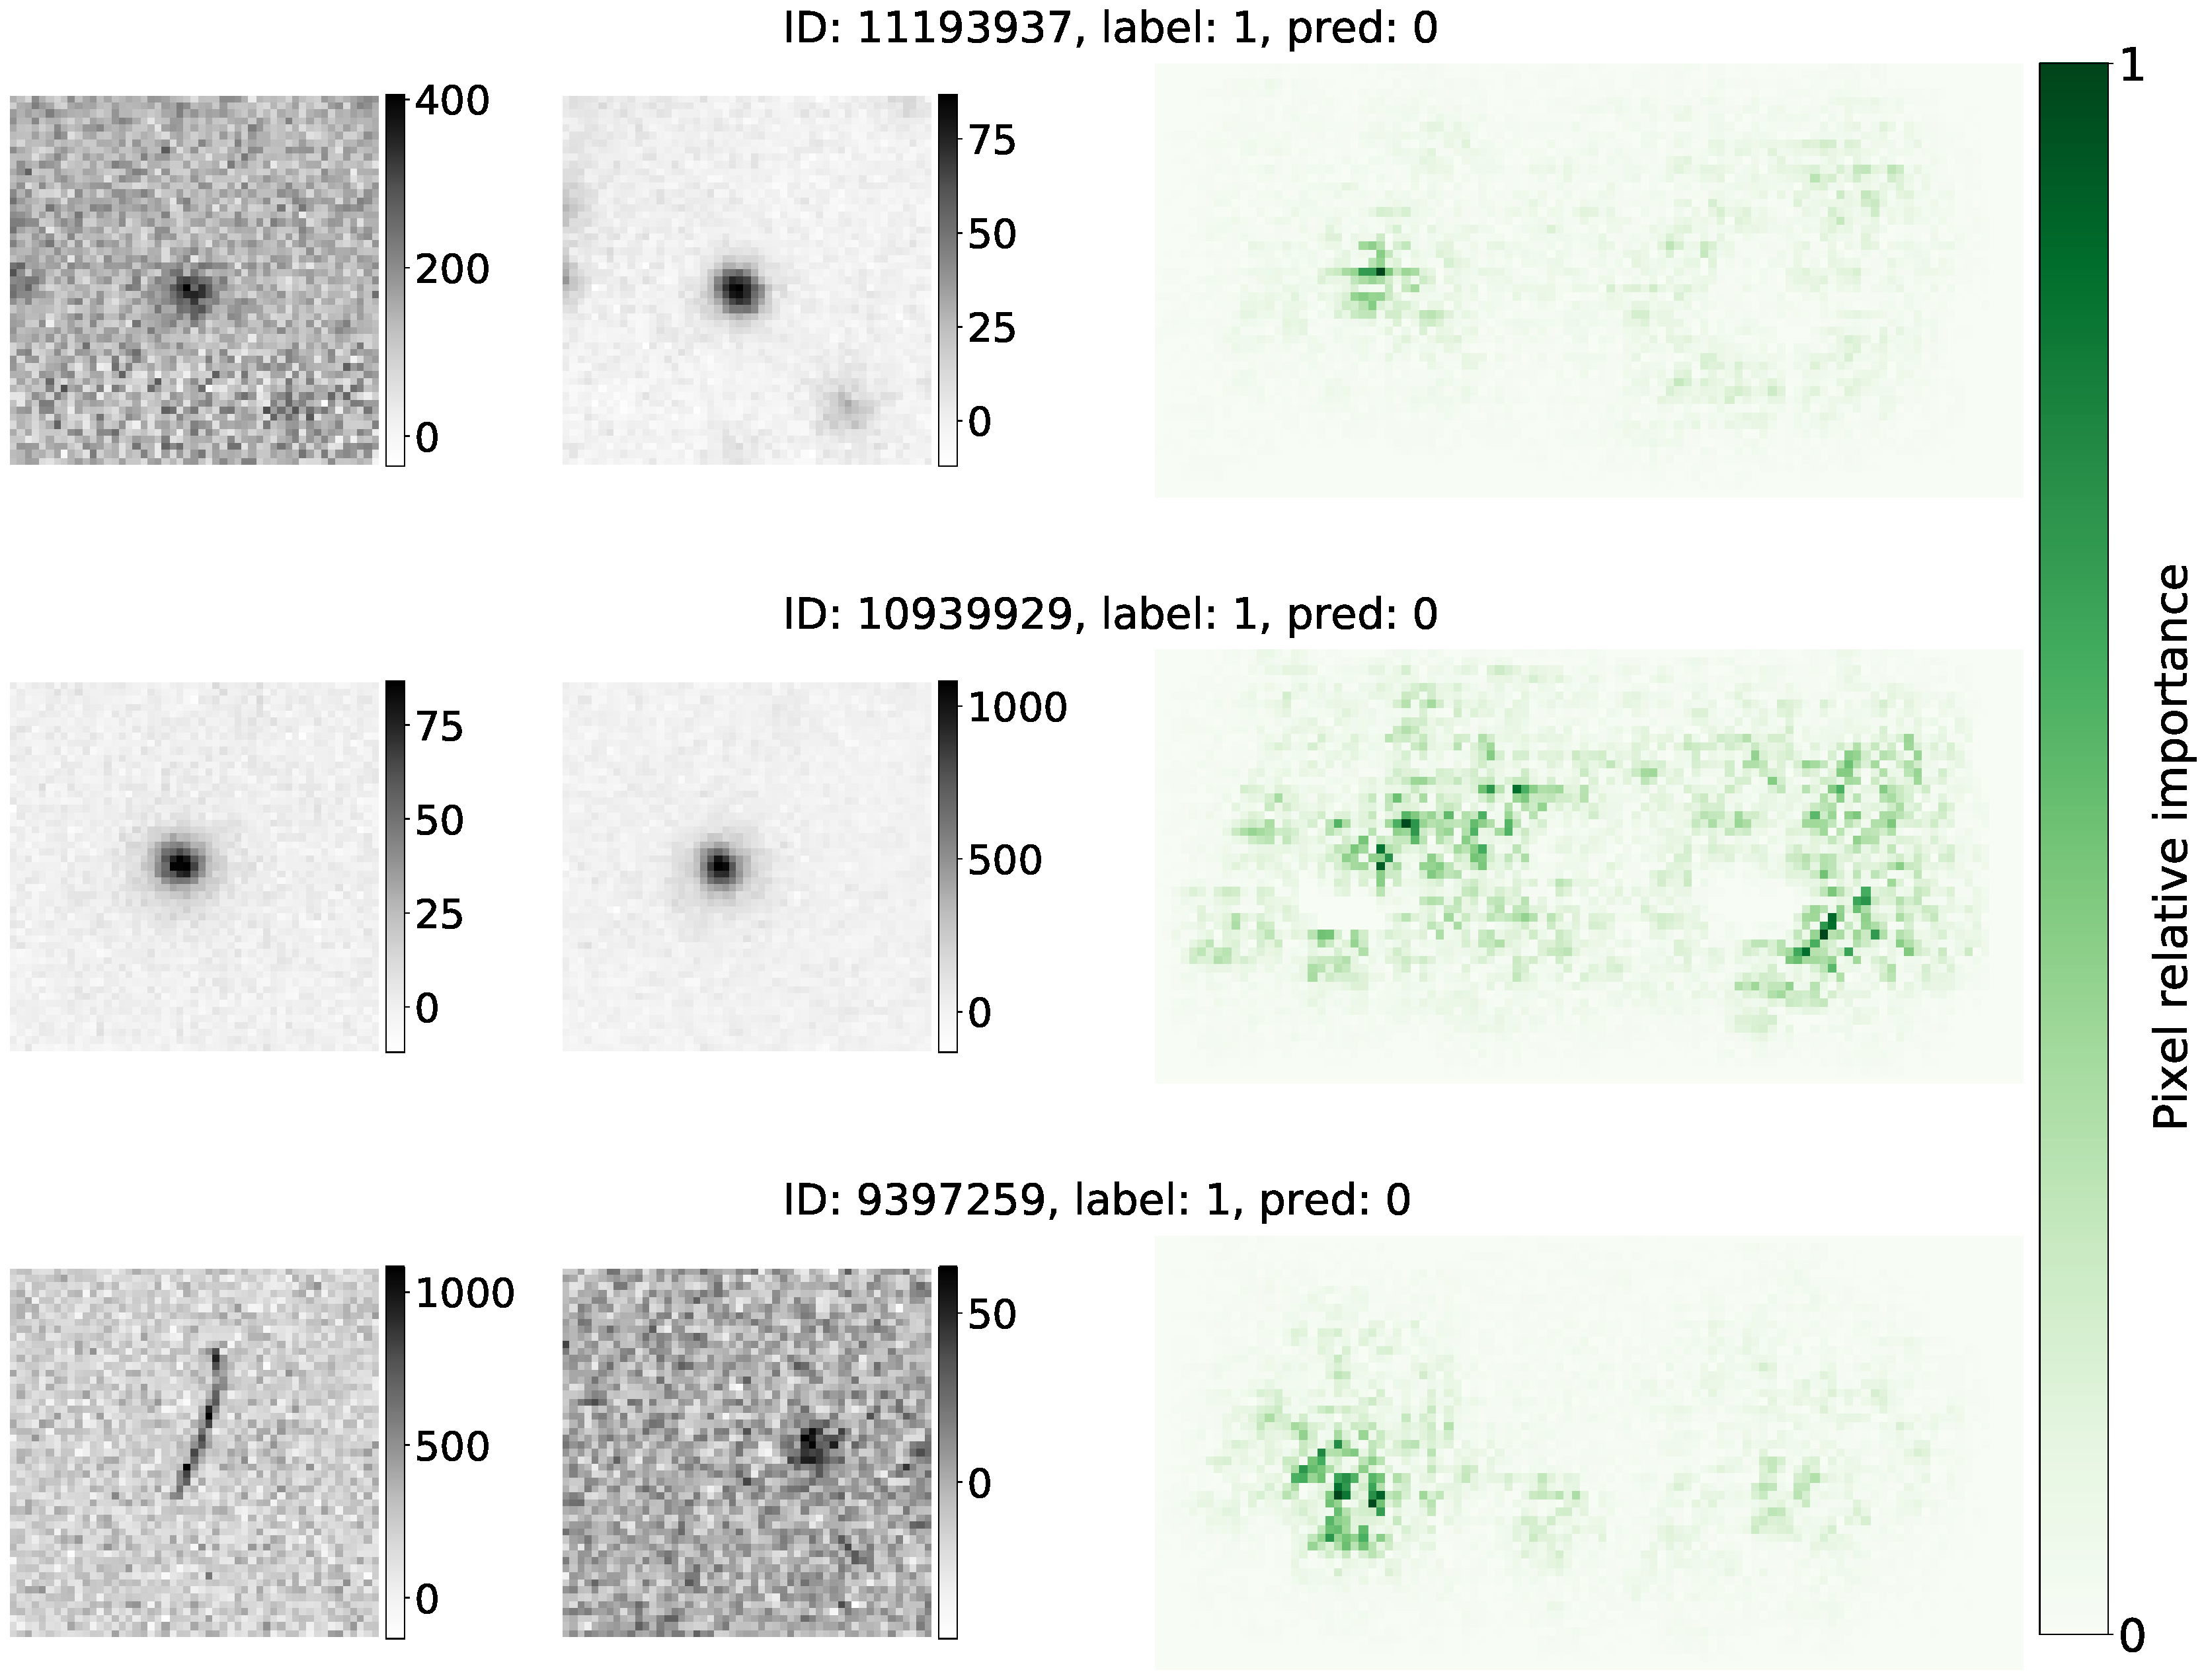
\includegraphics[width=0.76\linewidth]{
    figures/saliency_plot_other3nodiaFP-see854.pdf}
    \caption{Transients (\search-\temp) and their respective saliency map for the \nodia\ model False Positives (``bogus''  classified as ``real''). Important pixels are found everywhere in the image, as the CNN learns how to compare the \diff\ and \temp\ taking a synoptic look at the properties of each image component.}
    \label{fig:fpndia}
\end{figure*}



%\bibliographystyle{mnras}




\end{document}
